\documentclass[a4paper]{report}
\input{../../Templates/preamble.tex}
%PER CAMBIARE I MARGINI
\usepackage[margin=4cm]{geometry}

%----------- Setup stilistico ----------------
\definecolor{DarkRed}{HTML}{B6321C}
\hypersetup{
    colorlinks=true,
    linkcolor=DarkRed,
    filecolor=blue,
    citecolor = black,
    urlcolor=cyan,
}
\renewcommand\thefootnote{\textcolor{blue}{\arabic{footnote}}}
% ============================================


%---------- Comandi specifici ----------------


%--------- Comandi dattilografici ------------


% ============================================
\title{Sistemi Dinamici\\
\large Corso dei proff. Claudio Bonanno \& Roberto Castorrini}

\author{Francesco Sorce}
\date{Università di Pisa\\
Dipartimento di Matematica\\
A.A. 2023/24}

\begin{document}
\maketitle

%\newpage
\tableofcontents
\newpage
\chapter*{Introduzione}


\begin{definition}[Sistema dinamico]
Un \textbf{sistema dinamico} \`e una terna $(X,G,S)$, dove $X$ \`e un insieme, $G$ un (semi)gruppo e $S=G\acts X$ una azione.\\
L'insieme $X$ \`e detto \textbf{spazio delle fasi}.
\end{definition}
\begin{remark}
In realt\`a vorremmo che l'azione abbia una regolarit\`a compatibile con la struttura dell'insieme in esame.
\end{remark}


\section*{Sistemi continui}
\begin{definition}[Equazione differenziale]
Un \textbf{sistema di equazioni differenziali} (in forma esplicita) \`e un'equazione della forma
\[\dot x=F(x),\quad x\in\R^d, \ F\in C^1(\R^d).\]
Un \textbf{problema di Cauchy} associato all'equazione differenziale sopra \`e dato da un sistema del tipo
\[\begin{cases}
\dd t{}x(t)=F(x(t))\\
x(0)=x_0
\end{cases}\]
Per il teorema di Cauchy-Lipschitz \`e ben definito il \textbf{flusso} $\phi:\R^d\times \R\to \R^d$ associato all'equazione differenziale definito come la funzione che rispetta 
\[\begin{cases}
\dd t{}\phi_t(x_0)=F(\phi_t(x_0))\\
\phi_0(x_0)=x_0
\end{cases}.\]
\end{definition}

\begin{remark}
Osserviamo che $\phi_0:\R^d\to \R^d$ \`e la mappa identit\`a e che $\phi_{\cdot}(x)$ \`e un omomorfismo per ogni $x$, cio\`e
\[\phi_t(\phi_s(x))=\phi_{s+t}(x).\]
\end{remark}

\begin{definition}[Sistema dinamico a tempo continuo]
Una terna $(\R^d,\R,\phi_t(\cdot))$ \`e un \textbf{sistema dinamico (a tempo) continuo} se $\phi_t(\cdot)$ \`e il flusso di un sistema di ODE della forma $\dot x=F(x)$ con $F(x)$ campo di vettori, $F\in C^k$ con $k\geq1$.
\end{definition}


\begin{example}[Equazioni differenziali su $\R$]
Consideriamo l'equazione
\[\dot x=ax.\]
Il nostro approccio standard \`e imporre una condizione di Cauchy $x(0)=x_0$ e troviamo la soluzione
\[x(t)=x_0e^{at}.\]
Ponendo $G=\R,\ X=\R$ e $S=G\acts X$ dove $S(t,x_0)=\phi_t(x_0)$ possiamo interpretare l'equazione sopra come un sistema dinamico.

\noindent
Se consideriamo ora un'equazione del tipo
\[\dot x=a(x+x^9)\]
diventa difficile risolvere l'equazione. Possiamo fare studi qualitativi.

\noindent Negli studi qualitativi per $X=\R$ sono utili le seguenti considerazioni
\begin{itemize}
\item Rintracciare punti fissi
\item Studiare il segno della derivata
\item Soluzioni diverse non si incrociano per unicit\`a locale
\item Teorema di approssimazione lineare.
\end{itemize}
\end{example}

\noindent Di solito ci interesseranno equazioni in $\R^2$ o $\R^3$. Seguono alcuni modi per trasformare alcuni tipi di equazioni differenziali nella forma $\dot \ulx=\ul F(\ulx)$\footnote{Non metter\`o mai pi\`u le barre se posso.}.
\begin{example}[Ordine superiore]
Consideriamo l'equazione
\[\ddot x=-kx,\quad k>0.\]
Ponendo $y=\dot x$ troviamo
\[\begin{cases}
\dot x=y\\
\dot y=-kx
\end{cases}\coimplies \dot{\spa{\emat{x\\y}}}=\mat{y\\-kx}.\]
\end{example}

\begin{example}[Sistema non autonomo]
Consideriamo l'equazione
\[\dot x=f(x)+g(t)\]
Possiamo allargare lo spazio delle fasi come segue
\[\begin{cases}
\dot x=f(x)+g(t)\\
\dot t=1
\end{cases}.\]
\end{example}

%\noindent Per completezza mostriamo un sistema dinamico continuo che non deriva da una equazione differenziale:
%\begin{example}
%Ricordiamo la seguente
%\begin{definition}[Gruppo speciale lineare]
%Il gruppo speciale lineare a coefficienti in $R$ e dimensione $d$ \`e
%\[SL(d,R)=\cpa{M\in M(d,R)\mid \det M=1}.\]
%\end{definition}
%\noindent
%Consideriamo il seguente sistema dinamico: 
%\[X=SL(2,\R),\ G=\cpa{\mat{e^t & 0\\ 0 & e^{-t}}\mid t\in \R}\quad \text{e}\quad S:\funcDef{G\times X}{X}{(a,g)}{ga}.\]

%Consideriamo invece $X=\quot{SL(2,\R)}{SL(2,\Z)}$ [FINISCI NEL CASO]
%\end{example}

\section*{Sistemi discreti}
Definiamo ora sistemi dinamici discreti
\begin{definition}[Sistema dinamico a tempo discreto]
Un \textbf{sistema dinamico (a tempo) discreto} \`e una terna $(X,\N,T)$ dove $X\in\{\R,\ [a,b],\ S^1\}$ e $T:X\to X$ continua. Il sistema dinamico \`e dato da $(X,\N, S)$ dove $S(n,x)=T^n(x)$.
\end{definition}
\begin{remark}
Se $T$ \`e invertibile possiamo estendere un sistema dinamico discreto sostituendo $\N$ con $\Z$ e ponendo (per $n\in\N^+$) $S(-n,x)=(T\ii)^n(x)$.
\end{remark}

\begin{example}[Successione per ricorrenza]
Una successione per ricorrenza \`e un sistema dinamico discreto
\[\begin{cases}
x_n=T(x_{n-1})\\
x_0=a
\end{cases}\]
\end{example}

\begin{example}[Mappa di Bernoulli]
Consideriamo
\[S^1=\cpa{z\in\C\mid \abs z=1},\quad T:\funcDef{S^1}{S^1}{z}{z^2}\]
Osserviamo che l'unico punto fisso \`e $0$, ma reiterando da un punto qualsiasi non c'\`e modo che la successione vi tendi. Inoltre la distanza tra punti si raddoppia ad ogni iterata (a meno del modulo). Questo \`e uno dei primi esempi di sistemi caotici.
\end{example}
\part{Sistemi continui}
\chapter{Insiemi invarianti, Orbite e Omega-limiti}

\section{Orbite, punti fissi e periodici}
\begin{definition}[Orbita]
Definiamo l'\textbf{orbita positiva} del punto $x$ determinata da un'equazione di flusso $\phi$ come
\[\Oc^+(x)=\bigcup_{t\geq 0}\phi_t(x).\]
In modo simile definiamo l'\textbf{orbita negativa} e l'\textbf{orbita}.\\
La \textbf{traiettoria} di $x$ \`e il grafico $t\mapsto \phi_t(x)$ contenuto in $\R\times \R^d$\footnote{questa \`e la terminologia italiana. In inglese ''trajectory" corrisponde alla nostra orbita, non alla traiettoria.}.
\end{definition}

\begin{definition}[Punti fissi]
Un \textbf{punto fisso} $x\in\R^d$ \`e un punto tale che $F(x)=0$.
\end{definition}
\begin{remark}
L'orbita di un punto fisso \`e composta da un singoletto.
\end{remark}

\begin{definition}[Punti periodici]
Un punto $x\in\R^d$ \`e \textbf{periodico} se esiste $T>0$ tale che
\[\phi_{T+s}(x)=\phi_s(x)\quad \forall s\in\R\]
e $\phi_s(x)\neq x$ per ogni $s\in (0,T)$.\\
$T$ \`e detto \textbf{periodo minimo} di $x$.
\end{definition}
\begin{remark}
L'orbita di un punto periodico \`e data da
$\Oc(x)=\cpa{\phi_s(x)\mid s\in[0,T)}$.
\end{remark}

\begin{remark}[Simulazione]
Di solito per tracciare orbite usiamo il computer ma per natura di tali simulazioni, i dati iniziali (e l'integrazione stessa) non pu\`o essere assolutamente precisa. \`E quindi quasi impossibile disegnare algoritmicamente alcune orbite essenziali per comprendere il funzionamento del sistema (per esempio orbite periodiche, omo- ed eterocline e orbite limite tra due comportamenti). 
\end{remark}

\section{Insiemi invarianti}
\begin{definition}[Insiemi invarianti]
Un insieme $A\subseteq \R^d$ si dice \textbf{positivamente invariante} se per ogni $x\in A$, $\phi_t(x)\in A$ per ogni $t\geq 0$. In modo simile definiamo insiemi \textbf{negativamente invarianti} e \textbf{invarianti}.
\end{definition}

\begin{remark}[Le orbite sono invarianti]
Le orbite positive sono positivamente invarianti, le orbite negative sono negativamente invarianti e le orbite sono invarianti.
\end{remark}
\begin{proof}
Segue dal fatto che $\phi_{s+t}(x)=\phi_s(\phi_t(x))$.
\end{proof}

\begin{definition}[Integrale primo]
Una funzione $I:\R^d\to \R,\ I\in C^1(\R^d)$ \`e un integrale primo per $\dot x=F(x)$ se per ogni $x\in\R^d$
\[\dot I(x)\doteqdot \ps{\nabla I(x),F(x)}=\rbar{\dd{t}{}I(\phi_t(x))}_{t=0}=0.\]
\end{definition}



\begin{proposition}[Costruzione di insiemi invarianti da curve di livello]\label{CostruzioneInsiemiInvariantiCurveDiLivello}
Sia $c\in\R$ e $I:\R^d\to \R,\ I\in C^1$ tale che $\nabla I\res{\cpa{I=c}}\not\equiv 0$ e $\dot I\res{\cpa{I=c}}=0$, allora $\cpa{I=c}$ \`e invariante.
\end{proposition}
\begin{proof}
Sia $x_0\in I_c$. In particolare $\nabla I(x_0)\neq 0$. Senza perdita di generalit\`a supponiamo che l'ultima entrata sia non nulla, cio\`e $\pp{x_d}I(x_0)\neq 0$. Per il teorema della funzione implicita esistono un intorno $U$ di $x_0$ in $\R^d$ e una funzione $h:\R^{d-1}\to \R$ della stessa regolarit\`a di $I$ tali che\footnote{La mappa $\pi_{\neq x_d}$ \`e la proiezione ovvia da $\R^d$ a $\R^{d-1}$ che elimina l'ultima coordinata.}
\[I_c\cap U=\cpa{\ulx\in \pi_{\neq x_d}(U)\mid I(\ulx, h(\ulx))=c}.\]
A meno di restringere $U$, per il teorema sulla permanenza del segno supponiamo che $\pp{x_d}I\res{U}$ non si annulli mai.\\
Scriviamo $F=(\ulf,g)$ con $\ulf:\R^d\to \R^{d-1}$ e $g:\R^d\to\R$. Se $x_0=(\ulx_0,y_0)$, consideriamo il problema di Cauchy
\[\begin{cases}
\dot \ulx=\ulf(\ulx,h(\ulx))\\
\ulx(0)=\ulx_0
\end{cases}\]
e sia $\wt \psi_t(\ulx_0)$ la sua soluzione in un intorno di $\ulx_0$. Poniamo $\psi_t(x_0)=(\wt \psi_t(\ulx_0),h(\wt \psi_t(\ulx_0)))$ e verifichiamo che $\psi=\phi$. Chiaramente le condizioni iniziali coincidono, cos\`i come la derivata lungo le prime $d-1$ entrate. 
Per concludere basta dunque verificare che 
\[\dd t{}\pa{h(\wt \psi_t(\ulx))}=\Dc h(\wt\psi_t(\ulx))\wt\psi_t(\ulx)'=g(\ulx,h(\ulx)),\]
in quanto in tal caso avremo verificato che soluzioni che partono in $I_c\cap U$ restano in $I_c\cap U$ per tempi brevi.\\
Derivando $I(\psi_t(x_0))=c$ troviamo 
\[\nabla I(\psi_t(x_0))\cdot \mat{\ulf(\ulx,h(\ulx))\\\\\Dc h(\wt\psi_t(\ulx))\wt\psi_t(\ulx)'}=0\]
e dalla condizione $\dot I(\psi_t(x_0))=0$ ricaviamo
\[\nabla I(\psi_t(x_0))\cdot \mat{\ulf(\ulx,h(\ulx))\\g(\ulx,h(\ulx))}=0.\]
Confrontando queste due equazioni ricaviamo
\[\pp{x_d}I(\psi_t(x_0))\pa{\Dc h(\wt\psi_t(\ulx))\wt\psi_t(\ulx)'-g(\ulx,h(\ulx))}=0.\]
Poich\'e abbiamo supposto che $\pp{x_d}I\res{U}\neq 0$, da questa equazione ricaviamo l'uguaglianza cercata per un opportuno intorno di $x_0$.
\end{proof}

\begin{corollary}[Invarianza degli insiemi di livello di integrali primi]\label{InvarianzaInsiemiLivelloIntegraliPrimi}
Se $I$ \`e un integrale primo allora per ogni $c\in\R$ tale che $\nabla I\res{\cpa{I=c}}\neq0$ l'insieme
\[I_c=\cpa{I=c}\]
\`e invariante.
\end{corollary}


\begin{remark}[Intuizione geometrica]
Se $\nabla I(x)\neq 0$, la condizione $\dot I(x)=0$ afferma che $\nabla I(x)$ e $F(x)$ sono perpendicolari. Per il teorema delle funzioni implicite, se $x\in I_c$ abbiamo che un vettore normale a $I_c$ in $x$ \`e $\nabla I$, dunque se $F(x)$ vi \`e perpendicolare si ha che $F(x)\in T_x I_c$, in particolare l'orbita tende a procedere rimanendo nello spazio tangente, cio\`e resta contenuta in $I_c$.
\end{remark}

\section{Alpha e Omega limiti}
\begin{definition}[Alpha e Omega limiti]
Dato $x\in\R^d$ chiamiamo \textbf{$\omega$-limite} di $x$ l'insieme
\[\omega(x)=\cpa{y\in\R^d\mid \exists \{t_n\}\nearrow +\infty\ t.c.\ \lim_{k\to+\infty}\phi_{t_k}(x)=y}.\]
Similmente definiamo l'\textbf{$\alpha$-limite} considerando i limiti di successioni di tempi che vanno a $-\infty$.
\end{definition}
\begin{remark}
In realt\`a non \`e necessario chiedere successioni monotone. Per successioni generali che tendono a $\pm\infty$ basta passare a sottosuccessioni.
\end{remark}

\begin{example}
Seguono esempi di $\alpha$ e $\omega$ limiti semplici:
\begin{itemize}
\item Se $x$ \`e un punto fisso $\alpha(x)=\omega(x)=\cpa x$
\item Se $x$ \`e periodico $\alpha(x)=\omega(x)=\Oc(x)$
\end{itemize}
\end{example}

\begin{definition}[Omo-/etero-clino]
Siano $x_1$ e $x_2$ punti fissi e supponiamo $\cpa{x_1}=\alpha(y),\ \cpa{x_2}=\omega(y)$.\\ 
Se $x_1=x_2=x$ allora $y$ \`e detto \textbf{omoclino} di $x$.\\
Se $x_1\neq x_2$ allora $y$ \`e detto \textbf{eteroclino}.
\end{definition}

\begin{proposition}[Orbita limitata implica invarianza di $\omega$-limite]\label{OrbitaPositivaLimitataImplicaCompattezzaEInvarianzaOmegaLimite}
Se $x\in\R^d$ e $\Oc^+(x)$ \`e limitata allora $\omega(x)$ \`e non vuoto, compatto e invariante.
\end{proposition}
\begin{proof}
Sia $\cpa{\tau_j}\to+\infty$ tale che $\tau_1>0$ e $\tau_{j+1}>\tau_j$. 
Verifichiamo in linea preliminare la seguente uguaglianza:
\[\omega(x)=\bigcap_{j\geq 1}\ol{\Oc^+(\phi_{\tau_j}(x))}.\]
\setlength{\leftmargini}{0cm}  
\begin{itemize}
\item[$\boxed{\subseteq}$] Segue dal fatto che chiuso implica chiuso per successioni: per ogni $t\geq 0$ fissato vale definitivamente in $k$
\[\begin{cases}
y=\lim_k\phi_{t_k}(x)\\
\phi_{t_k}(x)\in \Oc^+(\phi_t(x))
\end{cases}\implies y\in \ol{\Oc^+(\phi_t(x))}\]
\item[$\boxed{\supseteq}$] Sia $y\in \bigcap_{j\geq 1}\ol{\Oc^+(\phi_{\tau_j}(x))}$. Per definizione di intersezione si ha che per ogni $j\geq 1$ abbiamo $y\in\ol{\Oc^+(\phi_{\tau_j}(x))}$. In particolare, per una caratterizzazione di chiusura in spazi metrici, esiste $t_j>0$ tale che
\[d(\phi_{t_j+\tau_j}(x),y)=d(\phi_{t_j}(\phi_{\tau_j}(x)),y)\leq \frac1j.\]
Segue che $\displaystyle\lim_{j\to+\infty}d(\phi_{t_j+\tau_j}(x),y)=0$, cio\`e $y\in \omega(x)$.
\end{itemize}
Verificata l'uguaglianza sopra, segue immediatamente che $\omega(x)$ \`e non vuoto e compatto (intersezione di compatti inscatolati non vuoti). Per mostrare l'invarianza mostriamo che $y\in\omega(x)\implies \phi_t(y)\in\omega(x)$ per ogni $t\in\R$.\\
Per definizione di $\omega$-limite esiste una successione $t_k\to+\infty$ tale che $\phi_{t_k}(x)\to y$. La tesi segue dalla seguente catena di identit\`a:
\[\phi_t(y)=\phi_t\pa{\lim_{k\to+\infty}\phi_{t_k}(x)}\overset{\text{continuit\`a in $t$}}=\lim_{k\to+\infty}\phi_{t+t_k}(x)\in\omega(x).\]
\end{proof}


\chapter{Stabilit\`a e funzioni di Lyapunov}
In questo capitolo e nel prossimo andiamo a studiare come si comportano i punti fissi\footnote{in questo studiamo la stabilit\`a, nel prossimo cercheremo quando possibile di descrive un comportamento pi\`u preciso}. Raccolte queste informazioni sui punti stabili speriamo di poterle poi ``incollare" per raggiungere un'idea sufficientemente accurata del comportamento dell'intero sistema.

\section{Stabilit\`a per Lyapunov}
\begin{definition}[Punti stabili per Lyapunov]
Un punto $x\in\R^d$ si dice 
\setlength{\leftmargini}{0.3cm}
\begin{itemize}
\item \textbf{stabile} (nel senso di Lyapunov) se per ogni $\e>0$ esiste $\delta>0$ tale che per ogni $y\in B_\delta(x)$ si ha che per ogni $t\geq 0$ abbiamo $\phi_t(y)\in B_\e(\phi_t(x))$.
\item \textbf{asintoticamente stabile} (nel senso di Lyapunov) se \`e stabile (nel senso di Lyapunov) ed esiste un intorno $U$ di $x$ tale che per ogni $y\in U$
\[\lim_{t\to+\infty}d(\phi_t(x),\phi_t(y))=0.\]
\item \textbf{instabile} (nel senso di Lyapunov) se non \`e stabile.
\end{itemize}
\setlength{\leftmargini}{0.5cm}
\end{definition}

\begin{remark}[Stabilit\`a per punti fissi]
Se $x$ \`e un punto fisso \`e stabile nel senso di Lyapunov se per ogni $\e>0$ esiste un $\delta>0$ tale che $d(y,x)<\delta\implies d(\phi_t(y),x)<\e$ per ogni $t\geq 0$. Similmente \`e asintoticamente stabile nel senso di Lyapunov se \`e stabile ed esiste un intorno $U$ tale che $\forall y\in U$ abbiamo $\displaystyle\lim_{t\to+\infty}\phi_t(y)= x$.
\end{remark}

\begin{definition}[Stabilit\`a orbitale]
Un insieme\footnote{preferibilmente positivamente invariante} $\Gamma\subseteq \R^d$ \`e \textbf{orbitalmente stabile} se per ogni $\e>0$ esiste $\delta>0$ tale che $d(y,\Gamma)<\delta\implies d(\phi_t(y),\Gamma)<\e$ per ogni $t\geq 0$.
\end{definition}

\begin{definition}[Dominio di asintotica stabilit\`a]
Se $x_0$ \`e un punto asintoticamente stabile definiamo il \textbf{dominio di asintotica stabilit\`a} come
\[\cpa{y\in\R^d\mid \omega(y)=\cpa{x_0}}.\]
\end{definition}

\begin{remark}[Convergenza non \`e sufficiente per asintotica stabilit\`a]
Esistono punti che rispettano la condizione di convergenza nella definizione di asintotica stabilit\`a che NON sono stabili (e quindi non vengono classificati come asintoticamente stabili).\\
Un punto di questo tipo \`e $(1,0)$ nel sistema (espresso in coordinate polari)
\[\begin{cases}
\dot\rho=\rho(1-\rho^2)\\
\dot\theta=2\sin^2\pa{\frac12\theta}
\end{cases}\]
\begin{figure}[!htb]
    \centering
    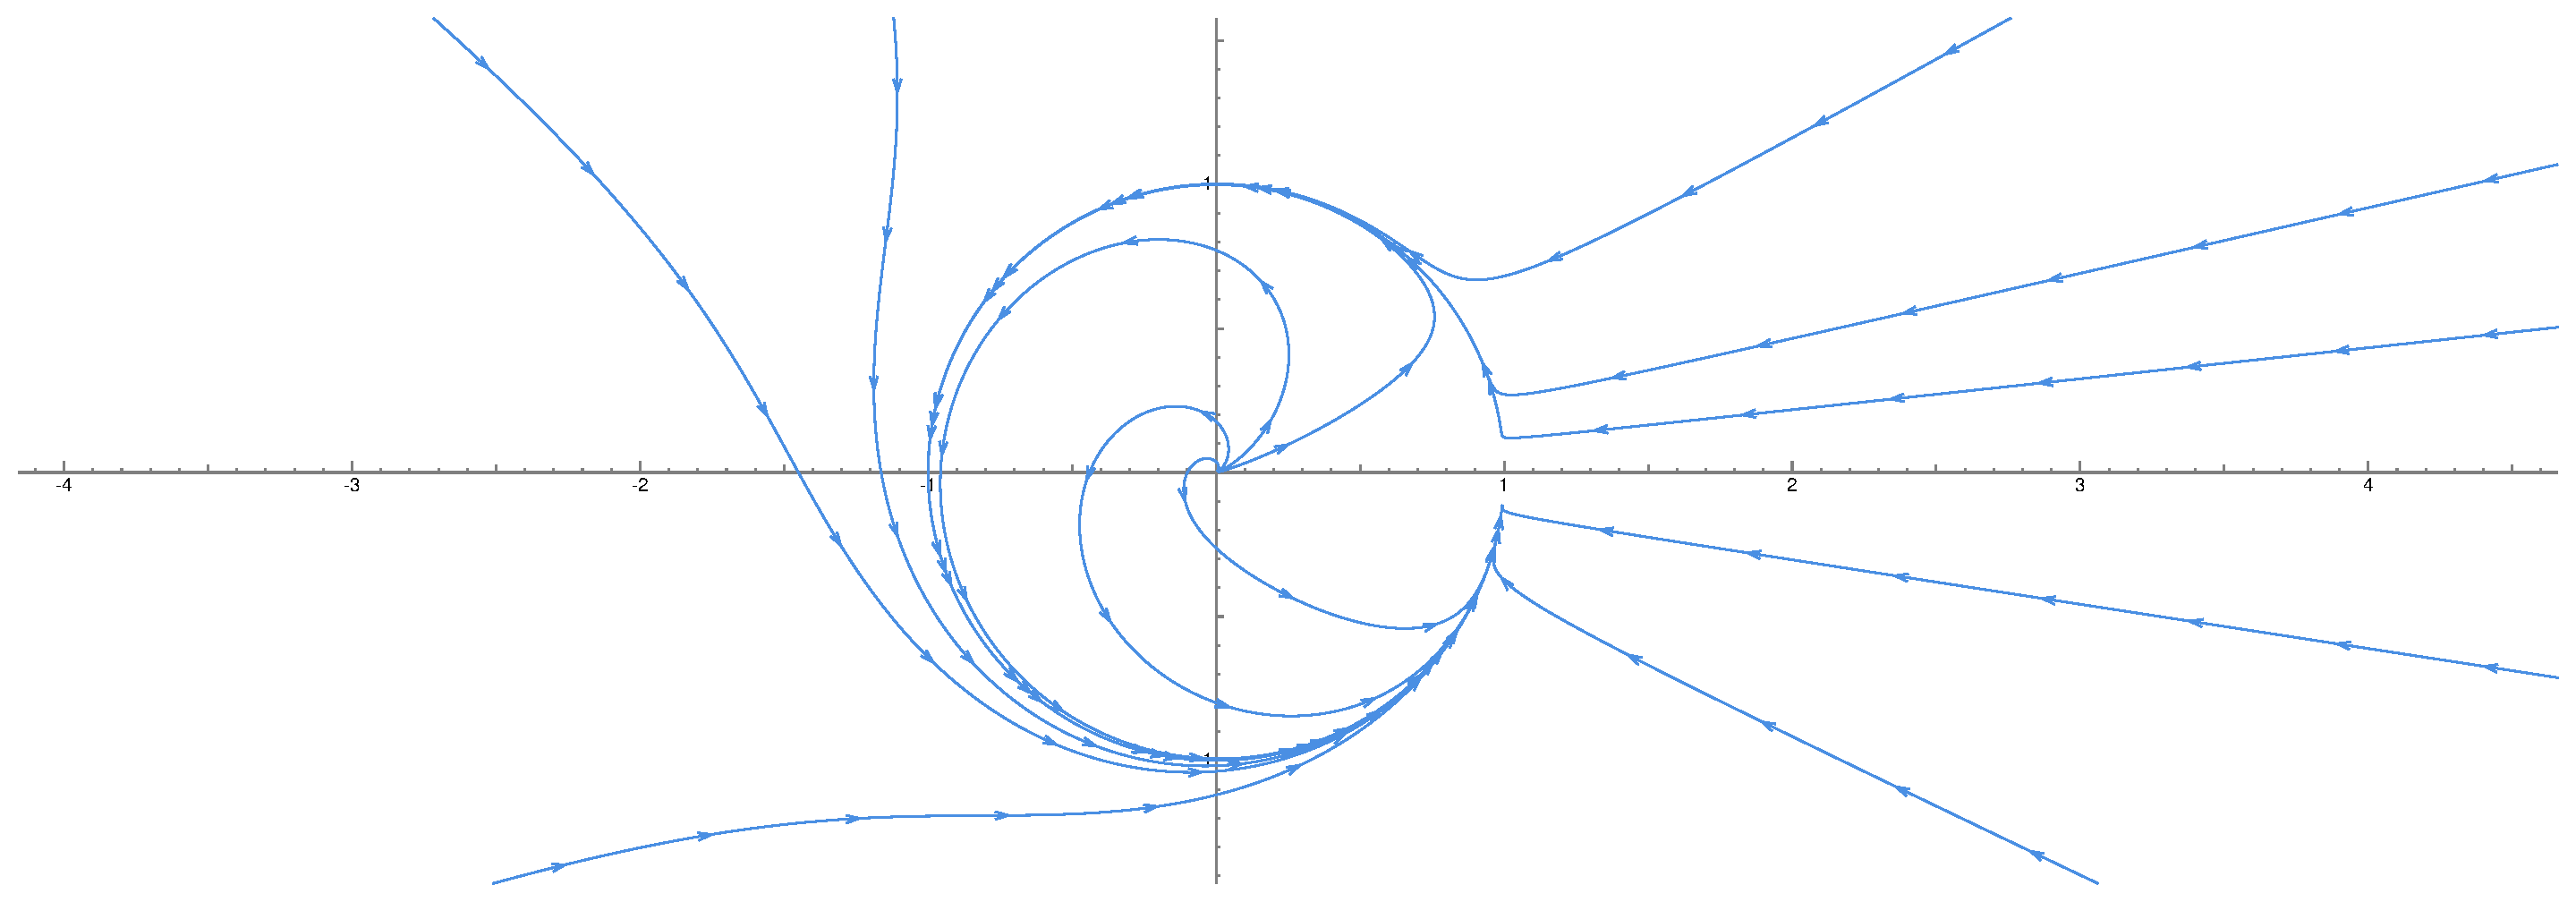
\includegraphics[width=11cm]{Immagini/convergenza_non_asintoticamente_stabile.pdf}
    \caption{In un intorno di $(1,0)$ ci sono sempre punti con $y>0$ e questi ``fanno un giro" prima di convergere.}
\end{figure}
\end{remark}

\section{Funzioni di Lyapunov}
\begin{definition}[Funzione di Lyapunov]
Sia $x_0\in\R^d$ punto fisso per $F\in C^1$ e $U(x_0)$ un suo intorno. Una funzione $V:U(x_0)\to\R$ si dice \textbf{funzione di Lyapunov per $x_0$} se $V\in C^1(U(x_0))$ e
\setlength{\leftmargini}{0.5cm}
\begin{itemize}
\item $V(x)>V(x_0)$ per ogni $x\in U(x_0)\bs \cpa{x_0}$
\item $\dot V(x)=\nabla V(x)\cdot F(x)\leq 0$ per ogni $x\in U(x_0)$.
\end{itemize}
Una funzione di Lyapunov \`e \textbf{stretta} se $\dot V(x)<0$ per ogni $x\in U(x_0)\bs \cpa{x_0}$.
\end{definition}

\begin{theorem}[Primo teorema di Lyapunov]\label{TeoremaLyapunov1Stabilita}
Sia $x_0\in\R^d$ un punto fisso per $F\in C^1$ e $V:U(x_0)\to\R$ una funzione di Lyapunov per $x_0$. Allora $x_0$ \`e un punto stabile nel senso di Lyapunov.
\end{theorem}
\begin{proof}
Fissiamo $\e>0$ tale che $\ol{B_\e(x_0)}\subseteq U(x_0)$. Definiamo \[m=\min_{\del B_\e(x_0)}V,\quad S_m=\cpa{y\in\ol{B_\e(x_0)}\mid V(y)< m}.\]
Osserviamo che $x_0\in S_m$ e, poich\'e $S_m=V\ii((-\infty,m))\cap B_\e(x_0)$, $S_m$ \`e aperto, dunque esiste $\delta>0$ tale che $B_\delta(x_0)\subseteq S_m$.\\
Sia ora $y\in B_\delta(x_0)$. Per definizione $V(y)< m$. Osserviamo che
\[\dd t{}V(\phi_t(y))=\dot V(\phi_t(y))\leq 0 \quad \forall t\geq 0\ t.c.\ \forall 0\leq s\leq t\ \phi_s(y)\in U(x_0),\]
in particolare, per gli stessi valori di $t$, $\phi_t(y)< m$ .\\
Per assurdo supponiamo che esista $\ol t>0$ tale che $\phi_{\ol t}(y)\notin B_\e(x_0)$. Per continuit\`a di $\phi_\cdot(y)$ possiamo supporre $\phi_{\ol t}(y)\in \del B_\e(x_0)$ e tale che per ogni $0\leq s\leq t$ si ha $\phi_s(y)\in U(x_0)$. Si ha dunque $V(\phi_{\ol t}(y))\geq m>V(\phi_t(y))$ per ogni $t\geq 0$ tale che $0\leq s\leq t$ abbiamo $\phi_s(y)\in U(x_0)$, ma $\del B_\e(x_0)\subset\ol B_\e(x_0)\subseteq U(x_0)$, da cui un assurdo.
\end{proof}

\noindent Introduciamo ora un criterio che \`e spesso utile per mostrare l'asintotica stabilit\`a:
\begin{proposition}[Criterio di La Salle]\label{CriterioLaSalle}
Sia $x_0$ un punto fisso per $F\in C^1$ e $V$ una funzione di Lyapunov per $x_0$ su $U(x_0)$. Se $y\in U(x_0)$ \`e tale che $\Oc^+(y)$ \`e limitata e contenuta in $U(x_0)$ allora $\omega(y)$ \`e un insieme non vuoto, compatto e invariante tale che $\omega(y)\subseteq \cpa{\dot V=0}$.
\end{proposition}
\begin{proof}
Se per $y$ valgono le ipotesi, per il criterio di invarianza per $\omega$-limiti (\ref{OrbitaPositivaLimitataImplicaCompattezzaEInvarianzaOmegaLimite}) abbiamo che $\omega(y)$ \`e non vuoto, compatto e invariante.\\
Osserviamo ora che $t\mapsto V(\phi_t(y))$ \`e non crescente e monotona, dunque esiste $\displaystyle c=\lim_{t\to+\infty}V(\phi_t(y))$. Osserviamo ora che
\begin{align*}
z\in \omega(y)&\coimplies \exists t_k\nearrow +\infty \ t.c.\ \phi_{t_k}(y)\to z\implies\\
&\implies V(z)=V\pa{\lim_{k}\phi_{t_k}(y)}\pasgnl={V\text{ cont.}}=\lim_k V(\phi_{t_k}(y))=c.
\end{align*}
Si ha dunque che $\omega(y)\subseteq \cpa{V=c}$. Per l'invarainza di $\omega(y)$ si ha che $V\circ \phi_\cdot(z)\res{\omega(y)}$ \`e costante per ogni $z\in\omega(y)$. Questo significa che $\dot V\res{\omega(y)}=0$, da cui $\omega(y)\subseteq \cpa{\dot V=0}$.
\end{proof}

\begin{remark}
Nelle ipotesi della proposizione, $x_0$ \`e stabile e quindi esiste un $y$ che rispetta le ipotesi.
\end{remark}

\begin{theorem}[Secondo teorema di Lyapunov]\label{TeoremaLyapunov2AsintoticaStabilita}
Sia $x_0\in \R^d$ un punto fisso per $F\in C^1$ e $V:U(x_0)\to\R$ una funzione di Lyapunov stretta per $x_0$, allora $x_0$ \`e asintoticamente stabile.
\end{theorem}
\begin{proof}
Per il primo teorema (\ref{TeoremaLyapunov1Stabilita}) abbiamo che $x_0$ \`e stabile, quindi dobbiamo solo verificare la convergenza.\\
Scelto $\e>0$ sia $\delta>0$ tale che $y\in B_\delta(x_0)$ e $\phi_t(y)\in B_\e(x_0)\subseteq U(x_0)$. Allora per La Salle (\ref{CriterioLaSalle}) $\omega(y)\subseteq \cpa{\dot V=0}\cap U(x_0)=\cpa{x_0}$.
\end{proof}

\begin{remark}
Se $V:U(x_0)\to\R$ \`e una funzione di Lyapunov stretta per $x_0$ allora
\[V_m=\cpa{y\in U(x_0)\mid V(y)\leq m}\]
\`e contenuto nel dominio di asintotica stabilit\`a per ogni $m$ tale che $V_{m}\subseteq U(x_0)$. In particolare vale per $V_{\wt m}$ dove
\[\wt m=\max\cpa{m\mid V_{m}\subseteq U(x_0)}.\]
\end{remark}

\begin{remark}
Se $x_0$ \`e un punto fisso
\setlength{\leftmargini}{0.5cm}
\begin{itemize}
\item Funzione di Lyapunov $\implies$ $x_0$ stabile
\item Funzione di Lyapunov stretta $\implies$ $x_0$ asintoticamente stabile
\item Funzione di Lyapunov + unico insieme invariante di $\cpa{\dot V=0}$ \`e il punto garantiscono comunque asintotica stabilit\`a (per il criterio di La Salle (\ref{CriterioLaSalle}))
\item Se $V:U(x_0)\to \R,\ V\in C^1(U(x_0))$ tale che $V(x)>V(x_0)$ per ogni $x\in U(x_0)\bs\cpa{x_0}$ e $\dot V(x)>0$ per ogni $x\in U(x_0)\bs\cpa{x_0}$ allora $x_0$ \`e \textit{instabile}.
\end{itemize}
\end{remark}

\subsection{Primo approccio per cercare funzioni di Lyapunov}
Nella risoluzione di esercizi spesso si vuole trovare una funzione di Lyapunov. Se non ci sono migliori metodi a disposizione per lo studio del punto, una scelta che di solito funziona quando pu\`o almeno localmente (per $y_0=(y_1,\cdots, y_d)$ punto fisso in esame) \`e
\[V(x_1,\cdots, x_d)=\sum_{i=1}^d a_i (x_i-y_i)^{2n_i},\]
cio\`e costruiamo un paraboloide sopra il punto fisso in esame. Gli insiemi di livello di questa funzione sono paraboloidi contenenti $y_0$.
\chapter{Linearizzazione}
\section{Idea della linearizzazione}
Per capire cosa aspettarci in un intorno di un punto fisso $x_0$ proviamo a linearizzare:
\[\dot x=F(x)=\under{=0}{F(x_0)}+\Dc F(x_0)(x-x_0)+o(\norm{x-x_0}).\]
Se $\norm{x-x_0}$ \`e abbastanza piccolo speriamo di trovare informazioni decentemente affidabili su $F(x)$ vicino a $x_0$ studiando $\Dc F(x_0)$.
\begin{example}[Esempio dove linearizzazione fallisce]
Linearizziamo il sistema dato da $F(x,y)=(x^2,x+y^2)$.
\[\Dc F(0,0)=\rbar{\mat{2x & 0\\ 1 &2y}}_{x=y=0}=\mat{0 & 0\\ 1&0},\]
quindi il sistema linearizzato ha equazione $G(x,y)=(0,x)$.
Problema: il sistema originale si comporta in modo un po' diverso nell'origine (acquisto una famiglia di punti fissi, orbite si deformano ecc\dots).
\begin{center}
    \begin{figure}[!htb]
        \centering
        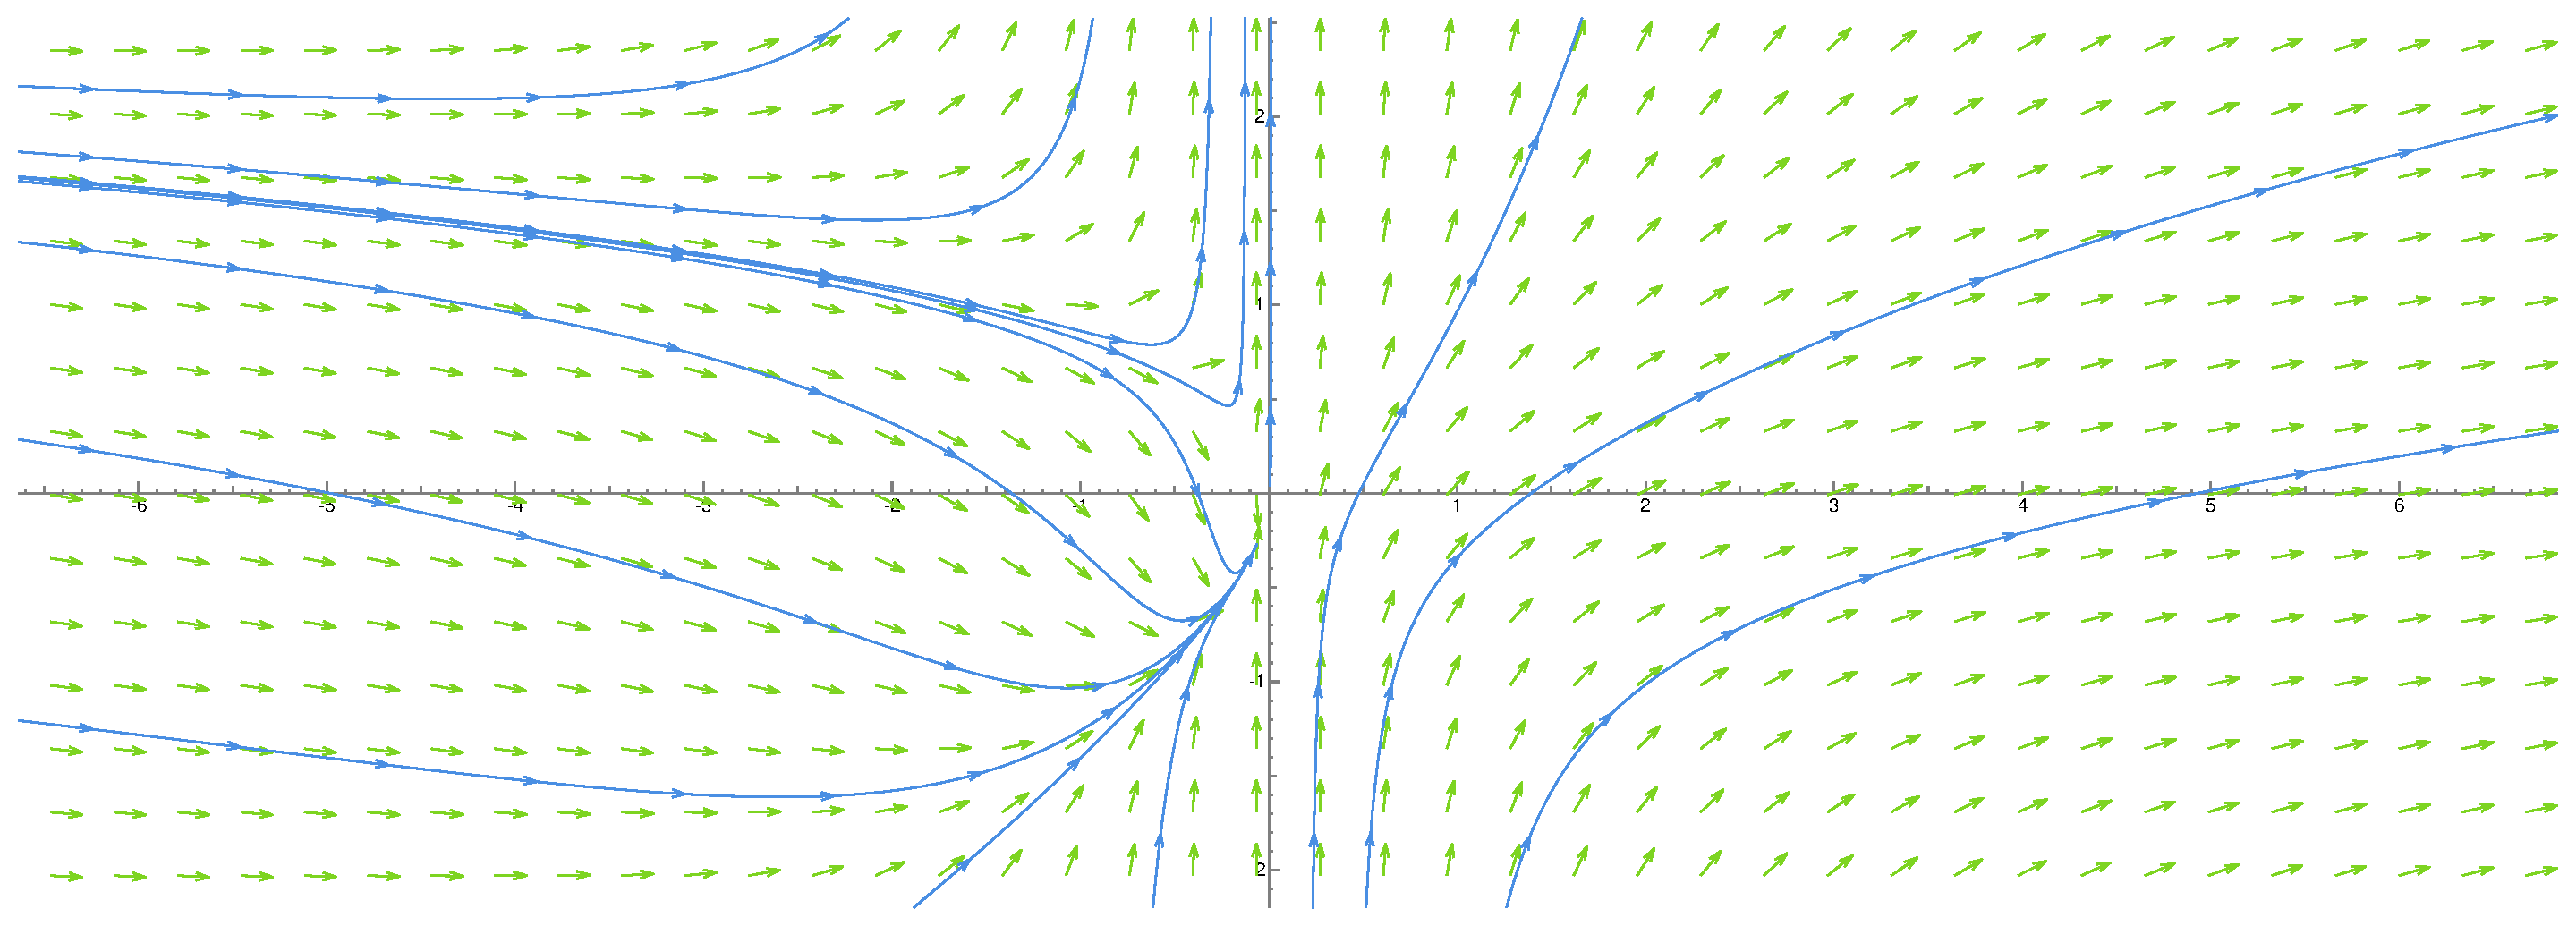
\includegraphics[height=2.8cm]{Immagini/fallita_linearizzazione.pdf}
    \end{figure}
    $\downarrow$
    \begin{figure}[!htb]
        \centering
        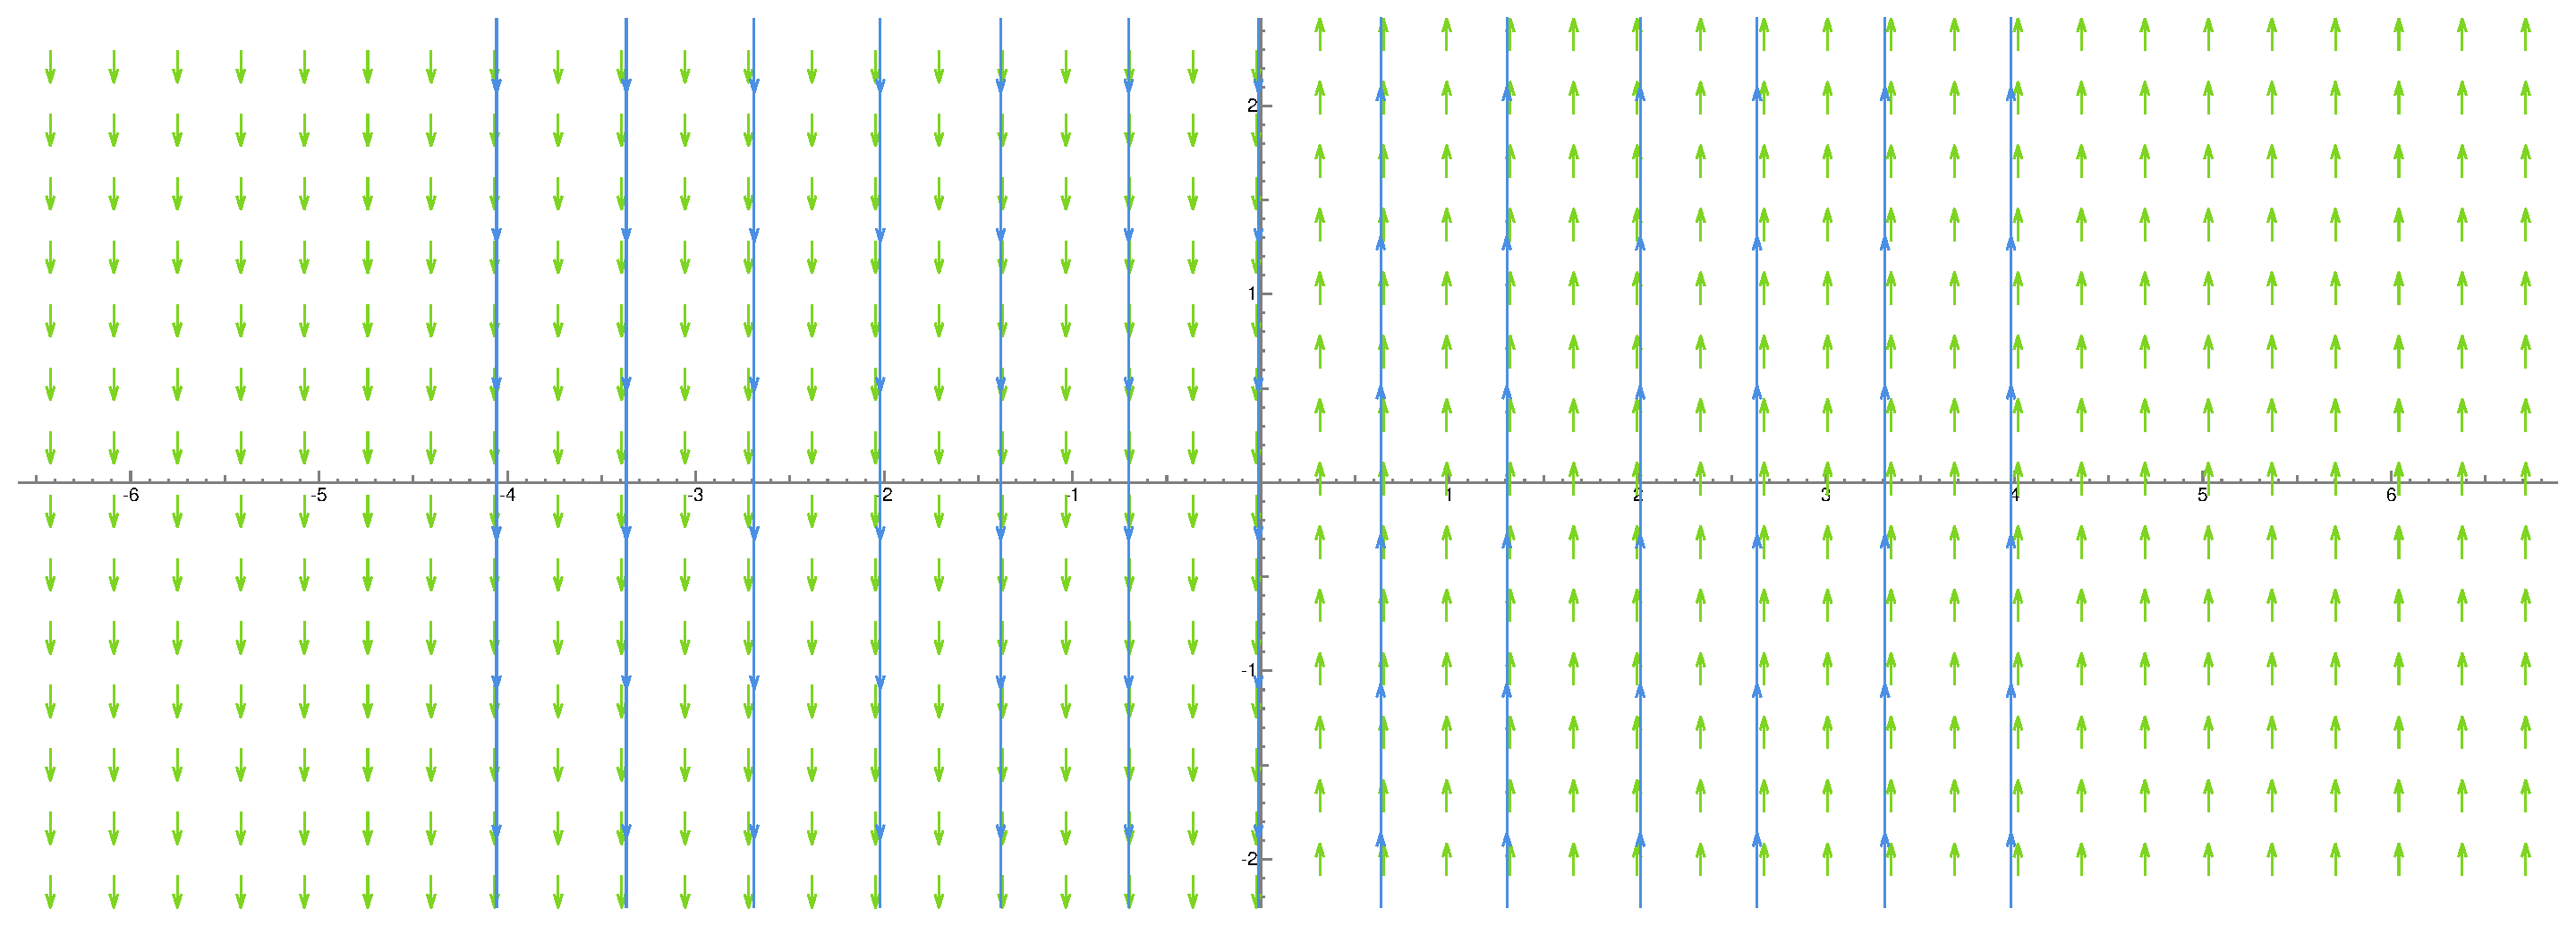
\includegraphics[height=2.8cm]{Immagini/fallita_linearizzazione_linearizzato.pdf}
    \end{figure}
\end{center}



\end{example}

\noindent Possiamo caratterizzare i punti stabili ``adatti allo studio tramite linearizzazione" dando la seguente definizione

\begin{definition}[Punti fissi iperbolici]
Un punto fisso $x_0\in\R^d$ per $F\in C^1$ si dice \textbf{iperbolico} se $\Dc F(x_0)$ non ha autovalori con parte reale nulla.
\end{definition}

\noindent Questi sono i punti ``buoni" perch\'e vale il seguente teorema.

\begin{theorem}[Hartman-Grobman]\label{TeoremaHartmanGrobman}
Sia $x_0\in\R^d$ un punto fisso iperbolico per $\dot x=F(x),\ F\in C^1$ e sia $\phi_t$ il flusso di questo sistema.\\
Consideriamo ora il \textbf{sistema linearizzato in $x_0$}, ovvero il sistema dato da
\[\dot y=\Dc F(x_0) y,\ y\in\R^d\]
e sia $\psi_t$ il flusso di questo sistema.\\
Esistono allora $U$ intorno di $x_0$, $V$ intorno di $0$ e un omeomorfismo $h:U\to V$ tale che per ogni $x\in U$ si ha che per ogni $t$ tale che $\phi_t(x)\in U$
\[h(\phi_t(x))=\psi_t(h(x)).\]
\end{theorem}
\begin{proof}
NON DATA DURANTE IL CORSO.
\end{proof}

\begin{remark}
La condizione $\Real(\la)=0$ \`e equivalente a $\abs{e^\la}=1$, cio\`e $e^\la=e^{i\theta}$. Intuitivamente questo ci dice che l'autospazio generalizzato corrispondente a $\la$ e $\ol\la$ non \`e attratto verso il punto fisso ma non vi \`e neanche respinto nel caso lineare, dunque nel sistema originale la sorte dei punti \`e determinata da espressioni non lineari.
\end{remark}

\begin{remark}
Anche se $F$ ha maggiore regolarit\`a, in generale $h$ non acquista regolarit\`a.
\end{remark}

\noindent
Ricordiamo il seguente
\begin{theorem}[Decomposizione in forma di Jordan reale]\label{JordanReale}
Sia $A\in\Mc(d,\R)$, allora esiste $P\in \Mc(d,\R)$ tale che $\det P\neq 0$ e $\Lambda=P\ii AP$ \`e diagonale a blocchi.
\end{theorem}
\noindent
Supponiamo che gli autovalori di $A$ siano in una delle seguenti forme
\begin{itemize}
\item $\{\la_j\}_{j\in\{1,\cdots, k\}}$ con $\la_j\in\R$ e $m_{alg}(\la_j)\leq 3$
\item $\cpa{a_j+ib_j}_{j\in\{1,\cdots, \ell\}}$ con $a_j,b_j\in\R$, $b_j\neq 0$ e $m_{alg}(a_j+ib_j)=1$.
\end{itemize}
Allora $\Lambda=diag(\Lambda_1,\cdots,\Lambda_k,B_1,\cdots,B_\ell)$ con
\begin{align*}
\Lambda_j\in&\cpa{\mat{\la_j & 1 & 0\\ 0&\la_j &1\\ 0&0&\la_j},\ \mat{\la_j & 1 & 0\\ 0&\la_j &0\\ 0&0&\la_j},\ \mat{\la_j & 0 & 0\\ 0&\la_j &0\\ 0&0&\la_j}}\cup\\
&\cup\cpa{\mat{\la_j & 1\\0&\la_j},\ \mat{\la_j&0\\0&\la_j},\mat{\la_j}}
\end{align*}
\[B_j=\mat{a_j & -b_j\\ b_j & a_j}.\]
Osserviamo che se $\dot y=\Dc F(x_0)y$ ed esiste $P$ invertibile tale che $P\ii \Dc F(x_0)P=\Lambda$ con $\Lambda$ in forma di Jordan reale allora, ponendo $z=P\ii y$ troviamo un omeomorfismo tale che
\[\dot z=P\ii \dot y=P\ii \Dc F(x_0)y=(P\ii\Dc F(x_0)P)z=\Lambda z.\]
\begin{notation}
Sia $V_{\la_j}$ l'autospazio generalizzato di $\la_j$, similmente per $a_j+ib_j$.
\end{notation}

\begin{proposition}[Gli autospazi generalizzati sono invarianti]\label{AutospaziGeneralizzatiSonoInvarianti}
Per $\dot y=Ay$, $A\in\Mc(d,\R)$ si ha che $V_{\la_j}$ e $V_{a_j+ib_j}$ sono insiemi invarianti.
\end{proposition}
\begin{proof}
Senza perdita di generalit\`a supponiamo che $A=\Lambda$ sia in forma di Jordan reale e a meno di permutare le coordinare mostriamo la tesi solo per $V_{\la_1}$\footnote{dove $\la_1$ in questo caso si riferisce ad autovalori potenzialmente complessi.}. Osserviamo che un generico vettore di $V_{\la_1}$ \`e della forma $y_0=((y_0)_1,\cdots, (y_0)_s, 0,\cdots, 0)$, dove $s=m_{alg}(\la_1)$ (dove poniamo $s=2$ nel caso di autovalore complesso). La tesi segue calcolando: 
\[\phi_t(y_0)=e^{t\Lambda}y_0=diag(e^{\Lambda_1 t},\cdots e^{\Lambda_s t})y_0=\mat{e^{\Lambda_1 t}\mat{(y_0)_1\\\vdots\\(y_0)_s}\\0\\\vdots\\0}\in V_{\la_1}.\]
\end{proof}

\begin{definition}[Sottospazi stabili]
Il \textbf{sottospazio stabile} di $0$ per il sistema $\dot y=Ay$ \`e l'insieme
\[E^s(0)=\Span(v\in V_{\la_i}\mid \Real(\la_i)<0).\]
Il \textbf{sottospazio instabile} ($E^u(0)$) e il \textbf{sottospazio centrale} ($E^c(0)$) sono definiti in modo analogo considerando $\Real(\la_i)>0$ e $\Real(\la_i)=0$ rispettivamente.
\end{definition}

\begin{theorem}[Invarianza e caratterizzazione dei sottospazi stabili]
Dato il sistema $\dot y=Ay$ si ha che:
\begin{enumerate}
\item $\dim E^u(0)+\dim E^s(0)+\dim E^c(0)=d$
\item $E^{s,c,u}(0)$ \`e invariante per $\phi_t$
\item $E^s(0)=\cpa{y_0\in\R^d\mid \displaystyle\lim_{t\to+\infty}\phi_t(y)=0}$
\item $E^u(0)=\cpa{y_0\in\R^d\mid \displaystyle\lim_{t\to-\infty}\phi_t(y)=0}$.
\end{enumerate}
\end{theorem}
\begin{proof}[Dimostrazione. (NON DATA DURANTE IL CORSO)]
Il primo punto segue da noti risultati sugli autospazi generalizzati.\\
Il secondo punto \`e una conseguenza dell'invarianza degli autospazi (\ref{AutospaziGeneralizzatiSonoInvarianti}).\\
Gli ultimi due punti seguono da come funzionano i $e^{\Real(\la)t}$ (questi fattori appaiono dopo essersi portati in forma di Jordan).
\end{proof}

\newpage
\section{Pozzi e Sorgenti}

\begin{definition}[Pozzi e sorgenti]
    Sia $x_0$ un punto fisso. Esso si dice
    \setlength{\leftmargini}{0.5cm}
    \begin{itemize}
        \item \textbf{pozzo} se ogni autovalore di $\Dc F(x_0)$ ha parte reale negativa,
        \item \textbf{sorgente} se ogni autovalore di $\Dc F(x_0)$ ha parte reale positiva.
    \end{itemize}
\end{definition}
    
\begin{remark}
    Si pu\`o pensare a sorgenti come pozzi per tempi negativi.
\end{remark}
    
\begin{proposition}[Stabilit\`a dei pozzi]\label{StabilitaPozzi}
    I pozzi sono asintoticamente stabili
\end{proposition}
\begin{proof}
    A meno di traslare il sistema supponiamo $x_0=0\in\R^d$.\\
    Poich\'e cambi di base lineari non cambiano la stabilit\`a dell'origine supponiamo che $\Dc F(0)$ sia in forma di Jordan reale. Trattiamo prima i casi dove $\Dc F(0)$ consiste di un solo blocco di Jordan e poi uniamo i risultati.
    \setlength{\leftmargini}{0cm}
    \begin{itemize}
        \item[$\boxed{\la\in\R}$] 
        Supponiamo che
        \[\Dc F(0)=\mat{
        \la & 1    &      &\\
            &\ddots&\ddots&\\
            &       &\la & 1\\
            &       &    &\la 
        }\implies \dot x=F(x)=\under{=0}{F(0)}+\Dc F(0)x+O(\norm x^2).\]
        Dato $\e>0$ consideriamo il cambio di base
        \[y=(y_1,\cdots, y_d),\quad y_i=\e^{-i+1}x_{i},\]
        da cui
        \[\dot y=A y+\wt G(y),\quad A=\mat{
        \la & \e    &      &\\
            &\ddots&\ddots&\\
            &       &\la & \e\\
            &       &    &\la 
        },\ {\wt G(y)}=O(\norm y^2).\]
        Affermiamo che la funzione
        \[V(y)=\frac12 \norm y^2\]
        \`e di Lyapunov stretta in un intorno di $0$. La prima condizione \`e evidentemente verificata, quindi dobbiamo solo trovare un intorno dove $\dot V(y)<0$ per $y\neq 0$.
        \begin{align*}
            \dot V(y)=&\sum_{i=1}^{d-1}y_i\under{\dot y_i}{(\la y_i+\e y_{i+1}+\wt G_i(y))}+y_d\under{\dot y_d}{(\la y_d+\wt G_d(y))}=\\
            =&\la\norm y^2+\e \sum_{i=1}^{d-1}y_iy_{i+1}+{y\cdot \wt G(y)}\pasgnlmath\leq{(\ast)}\\
            \leq& \la\norm y^2+\frac\e2 \pa{\sum_{i=1}^{d-1}y_i^2 +\sum_{i=2}^{d}y_i^2}+O(\norm y^3)=\\
            =&\pa{\la+\frac\e2}(y_1^2+y_d^2)+(\la+\e)\sum_{i=2}^{d-1}y_i^2+O(\norm y^3)\leq\\
            \leq& (\la+\e)\norm y^2+O(\norm y^3),
        \end{align*}
        dove nel passaggio evidenziato abbiamo usato 
        \[0\leq \norm{\mat{y_1-y_2\\\vdots\\y_{d-1}-y_d}}^2.\]
        Cerchiamo dunque condizioni valide per $\e$ e $\norm y$:\\
        Poich\'e $\la<0$ \`e lecito fissare $\e\in(0,\abs\la)$. Per le propriet\`a degli $O$ grandi esistono $r,C>0$ tali che
        \[\norm y<r\implies \dot V(y)\leq((\la+\e)+C\norm y)\norm y^2.\]
        Ponendo ora $\la+\e+C\norm y<0$ si ha che se 
        \[r'<\min\cpa{r,\frac{\abs{\la+\e}}{C}}\]
        allora per $y\in B_{r'}(0)\bs\cpa0$ vale
        \[\dot V(y)\leq ((\la+\e)+C\norm y)\norm y^2<0,\]
        cio\`e $V$ \`e una funzione di Lyapunov stretta per $x_0$ in un opportuno cambio di base, dunque $x_0$ \`e asintoticamente stabile per il secondo teorema di Lyapunov (\ref{TeoremaLyapunov2AsintoticaStabilita}).
        \item[$\boxed{\la\in\C\bs \R}$] Supponiamo che
        \[\Dc F(0)=\mat{
        \emat{a&b\\-b&a} & \emat{1&0\\0&1}     &      \\
            &\ddots &\ddots&\\
            &       &\ddots
        }\]
        A meno di un coniugio\footnote{nota che anche la matrice del cambio di base deve avere blocchi $2\times 2$.} troviamo
        \[\dot y=Ay+\wt G(y),\quad A=\mat{
        \emat{a&b\\-b&a} & \emat{\e&0\\0&\e}     &      \\
            &\ddots &\ddots&\\
            &       &\ddots
        }\]
        e concludiamo in modo simile al caso precedente.
        \item[$\boxed{\text{generale}}$] Segue dai due casi precedenti dando un'ulteriore limitazione con gli $O$ grandi sui termini non lineari.
    \end{itemize}
    \setlength{\leftmargini}{0.5cm}
\end{proof}

\section{Classificazione dei punti stabili lineari sul piano}
Consideriamo i sistemi lineari di questa forma
\[\dot x=Ax,\quad A\in\Mc(2,\R),\ x=\mat{u\\ v}\in\R^2.\]
Sappiamo che
\[\phi_t(x_0)=e^{At}x_0,\]
in particolare $x_0=0$ \`e un punto fisso.
\[A=\mat{a & b\\ c & d}\implies p_A(\la)=\la^2-(a+d)\la+ad-bc=\la^2-(\tr A)\la+\det A.\]
Segue che gli autovalori di $A$ sono
\[\la_{\pm}=\frac{\tr A\pm \sqrt{\Delta}}{2},\ \Delta=(\tr A)^2-4\det A.\]
Consideriamo i possibili casi:
\setlength{\leftmargini}{0cm}
\begin{itemize}
\item[$\boxed{\emat{\det A>0\\ \Delta>0}}$] Gli autovalori $\la_\pm$ sono reali distinti.\\
$\star)$ Se $\tr A>0$ allora $\la_+>\la_->0$, da cui a meno di coniugio
\[A=\mat{\la_+ &0\\0&\la_-}\implies \begin{cases}
\dot u=\la_+ u\\
\dot v=\la_- v
\end{cases},\]
da cui le soluzioni sono
\[(u(t), v(t))=(e^{\la_+t}u_0, e^{\la_-t}v_0).\]
Questa situazione \`e detta \textbf{nodo instabile}.\\ Osserviamo che $E^u(0)=\R^2$ e $E^s(0)=E^c(0)=\cpa0$.\\
$\star)$ Se $\tr A<0$ allora $\la_-<\la_+<0$ e troviamo il \textbf{nodo stabile}.\\ Osserviamo che $E^s(0)=\R^2$ e $E^u(0)=E^c(0)=\cpa0$.
\item[$\boxed{\emat{\det A>0\\ \Delta<0}}$] Gli autovalori $\la_\pm$ sono complessi coniugati. $\la_\pm=\al\pm i\beta$ con $\al,\beta\in\R$. Segue che $\tr A=2\al$. A meno di coniugio
\[A=\mat{\al & -\beta\\ \beta &\al}\implies e^{At}=e^{\al t}\mat{\cos(\beta t) & -\sin(\beta t)\\ \sin(\beta t) & \cos(\beta t)}.\]
$\star)$ Se $\al>0$ troviamo
\[x(t)=e^{\al t} R_{\beta t}(x_0)\]
cio\`e un \textbf{fuoco instabile}. Osserviamo che $E^u(0)=\R^2$ e $E^s(0)=E^c(0)=\cpa0$.\\
$\star)$ Se $\al<0$ troviamo
\[x(t)=e^{\al t} R_{\beta t}(x_0)\]
cio\`e un \textbf{fuoco stabile}. Osserviamo che $E^s(0)=\R^2$ e $E^u(0)=E^c(0)=\cpa0$.\\
$\star)$ Se $\al=0$ troviamo
\[x(t)=R_{\beta t}(x_0)\]
cio\`e un \textbf{centro}. Osserviamo che $E^c(0)=\R^2$ e $E^s(0)=E^u(0)=\cpa0$.
\item[$\boxed{\emat{\det A>0\\ \Delta=0}}$] Gli autovalori coincidono e sono della forma $\la=\tr A/2$. A meno di coniugio abbiamo due possibilit\`a:
\[A=\mat{\la &0\\0&\la}\implies x(t)=e^{\la t}x_0\]
Questa situazione \`e detta \textbf{Stella stabile/instabile} per segno negativo o positivo della traccia rispettivamente.
\[A=\mat{\la & 1\\ 0 &\la}\implies x(t)=e^{\la t}(u_0+t v_0, v_0).\]
Questa situazione \`e detta \textbf{nodo stabile/instabile improprio}.
\item[$\boxed{\emat{\det A<0\\ \Delta>0}}$] Gli autovalori sono reali di segno opposto $\la_-<0<\la_+$. A meno di coniugio
\[A=\mat{\la_+ &0\\ 0&\la_-}\implies x(t)=(u_0e^{\la_+t},v_0e^{\la_-t}).\]
Troviamo un \textbf{punto di sella}. Il segno della traccia specifica solo verso quale asse le iperboli sono schiacciate.\\
Osserviamo che $E^s(0)=\{x=0\},\ E^u(0)=\cpa{y=0},\ E^c(0)=0$, cio\`e lo ``spazio tangente" in $0$ si decompone in una retta stabile e una instabile.
\item[$\boxed{\det A=0}$] Gli autovalori sono $0$ e $\tr A$. In tutti i casi a meno di coniugio una coordinata resta costante, dunque troviamo delle \textbf{rette}.
\end{itemize}

\noindent Riassumiamo i casi nella seguente tabella
\begin{center}
\begin{tabular}{|c|c|c||c|}
\hline
$\sgn\det A$ & $\sgn \Delta$ & $\sgn \tr A$ & Nome\\\hline\hline
+ & + & + & Nodo instabile \\\hline
+ & + & - & Nodo stabile \\\hline
+ & - & + & Fuoco instabile \\\hline
+ & - & - & Fuoco stabile \\\hline
+ & - & 0 & Centro \\\hline
+ & 0 & + & Stella o nodo improprio instabile \\\hline
+ & 0 & - & Stella o nodo improprio stabile \\\hline
- & + & $\bullet$ & Punto di Sella \\\hline
0 & $\bullet$ & $\bullet$ & Rette \\\hline
\end{tabular}
\end{center}

\begin{figure}[!htb]
    \centering
    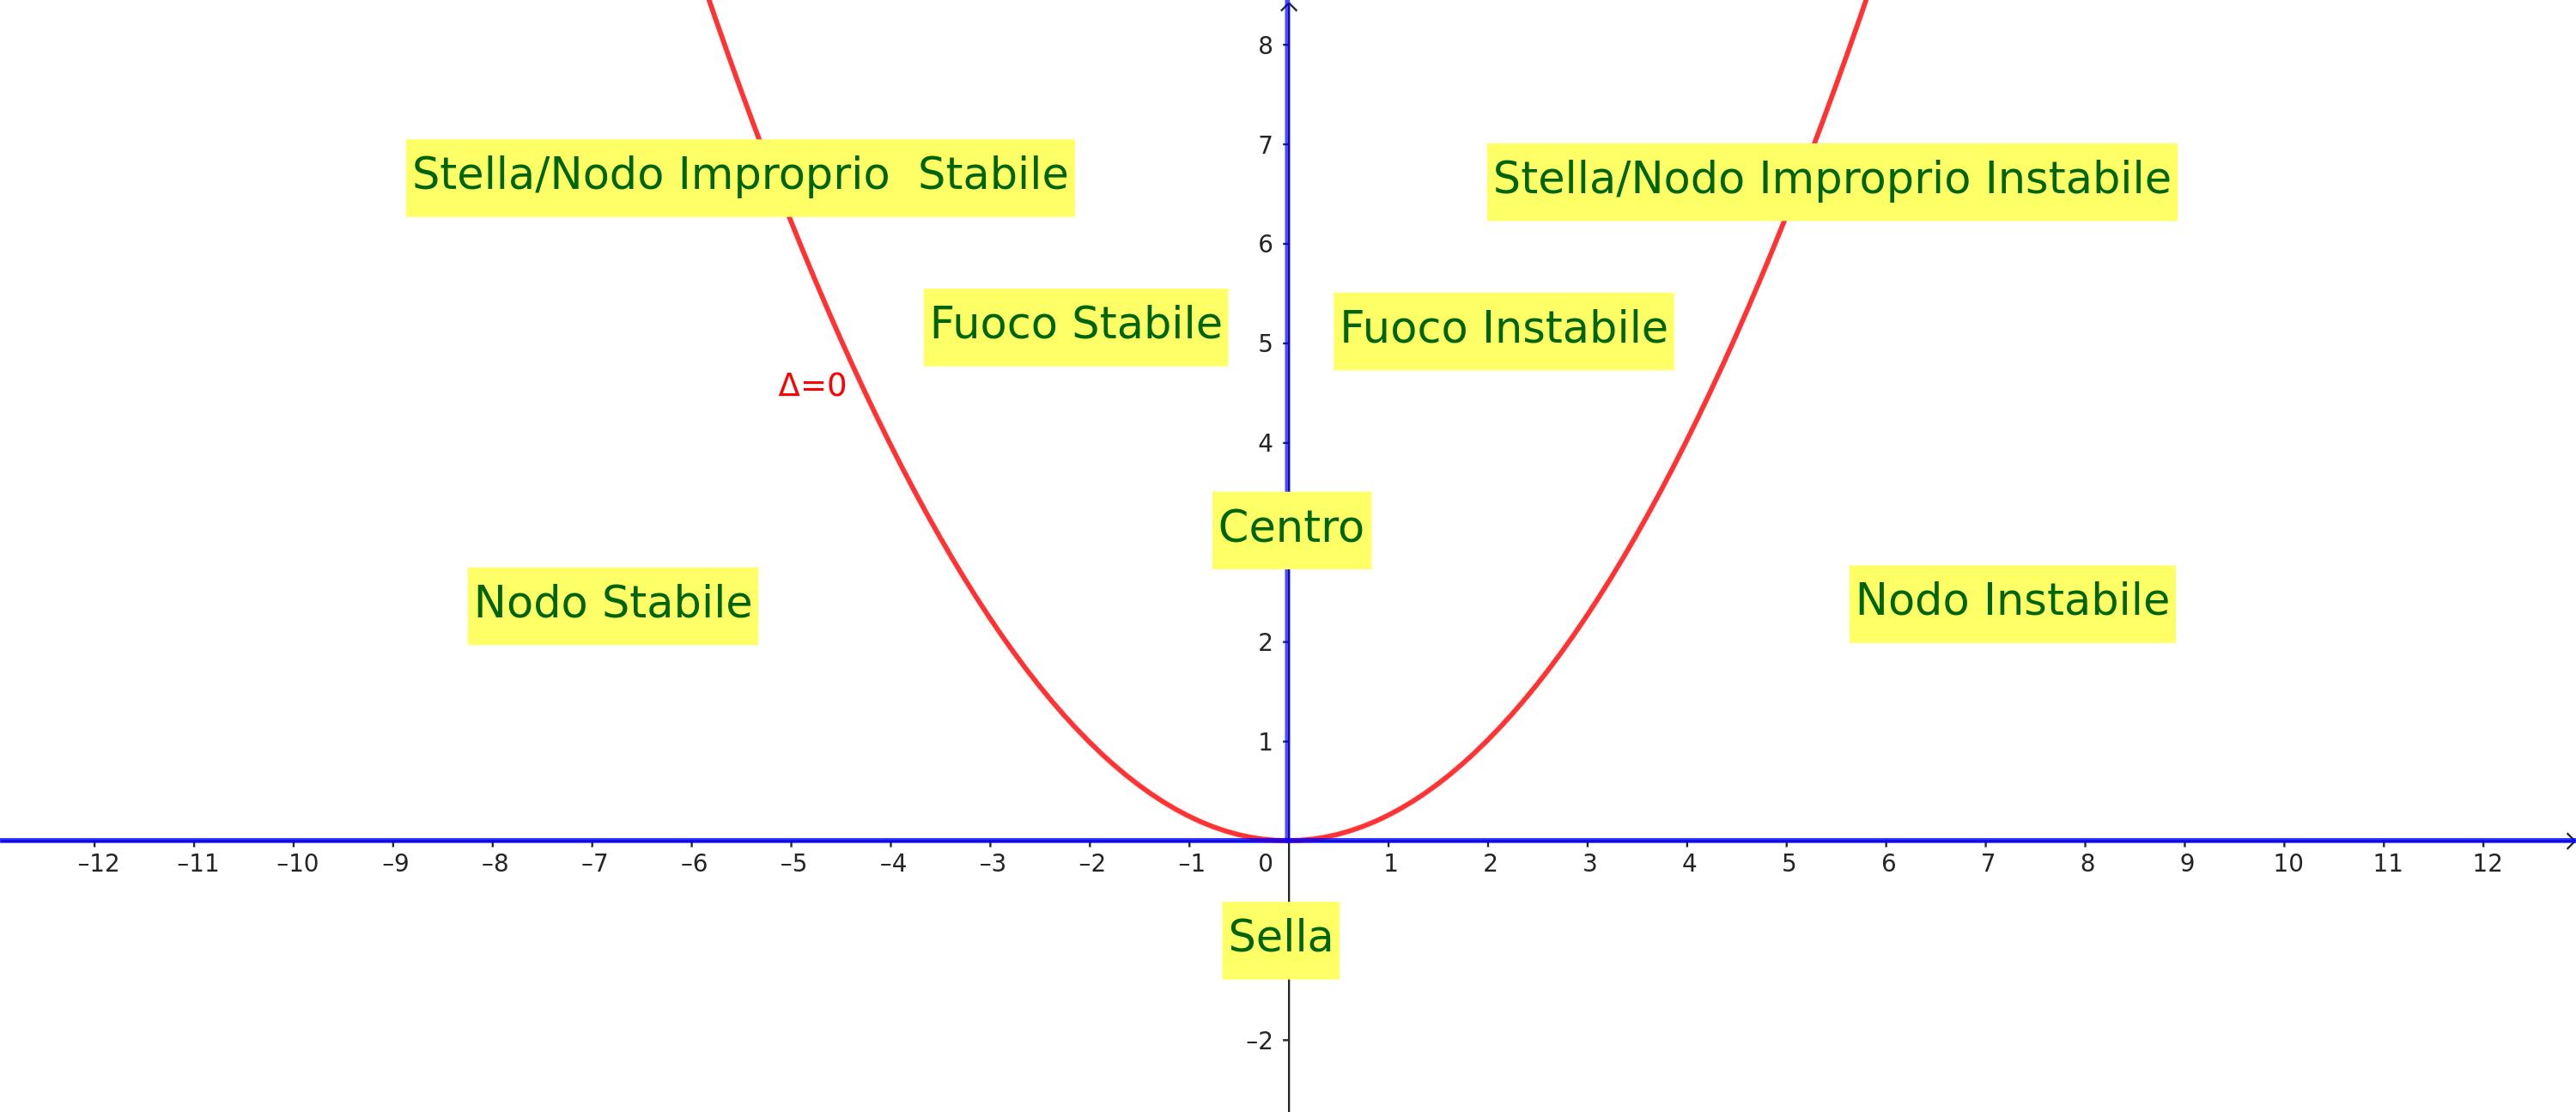
\includegraphics[width=\textwidth]{Immagini/Diagramma_punti_stabili_lineari.png}
    \caption{Utile diagramma che organizza i tipi di punti stabili lineari. L'asse $x$ corrisponde ai possibili valori di $\tr A$ e l'asse $y$ ai possibili valori di $\det A$. La parabola rossa indica il luogo dove $\Delta=0$; nella regione sopra la parabola troviamo $\Delta<0$ e sotto $\Delta>0$. In blu sono indicati i valori di $\tr A$ e $\det A$ per cui il punto stabile in considerazione NON \`e iperbolico.}
\end{figure}

\noindent Riportiamo dei diagrammi di fase per evidenziale la forma delle orbite.

\begin{figure}[!htb]
    \centering
    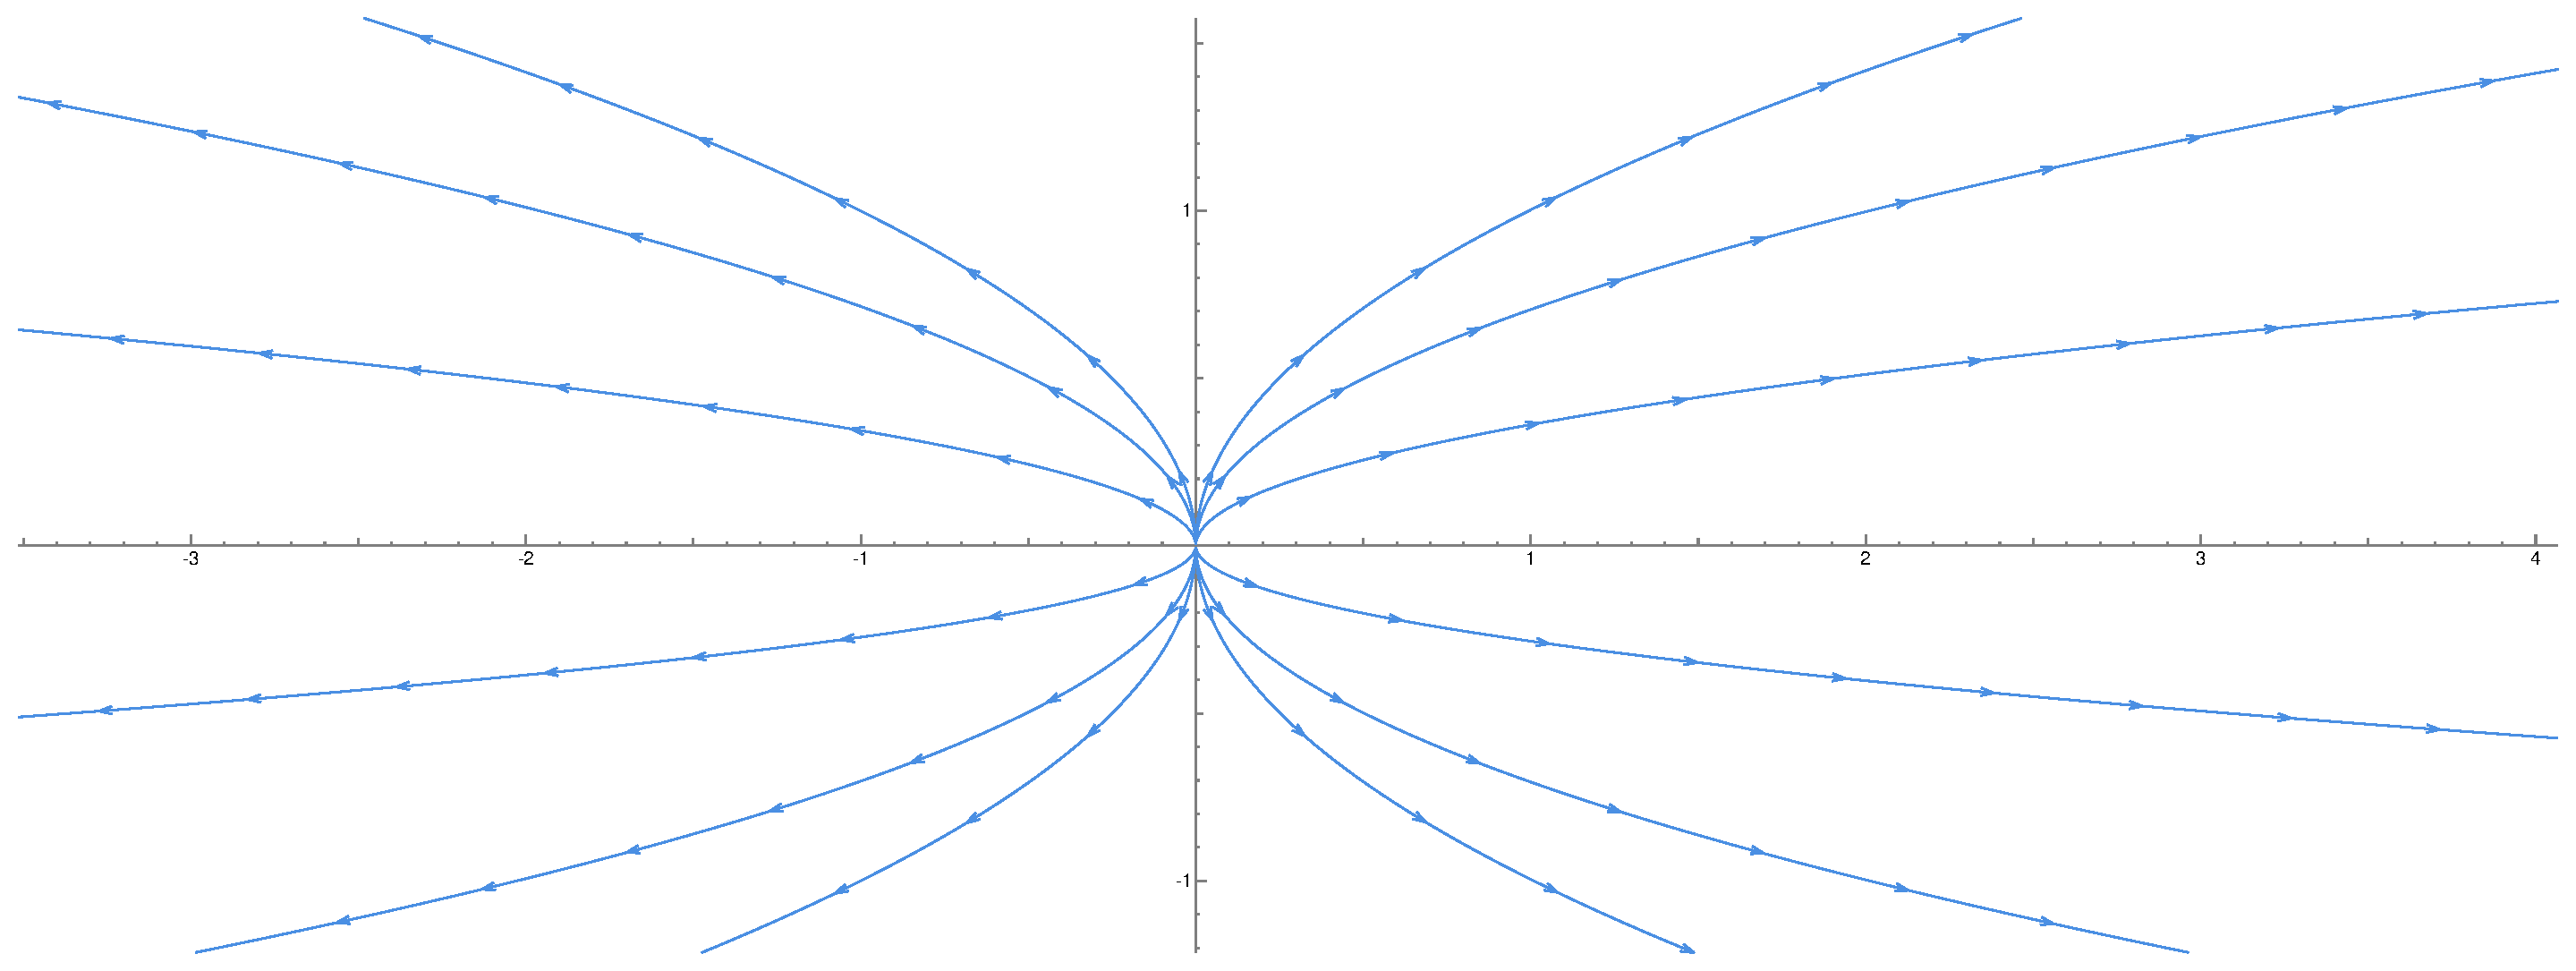
\includegraphics[width=11cm]{Immagini/nodo_instabile.pdf}
    \caption{Nodo instabile}
\end{figure}


\begin{figure}[!htb]
    \centering
    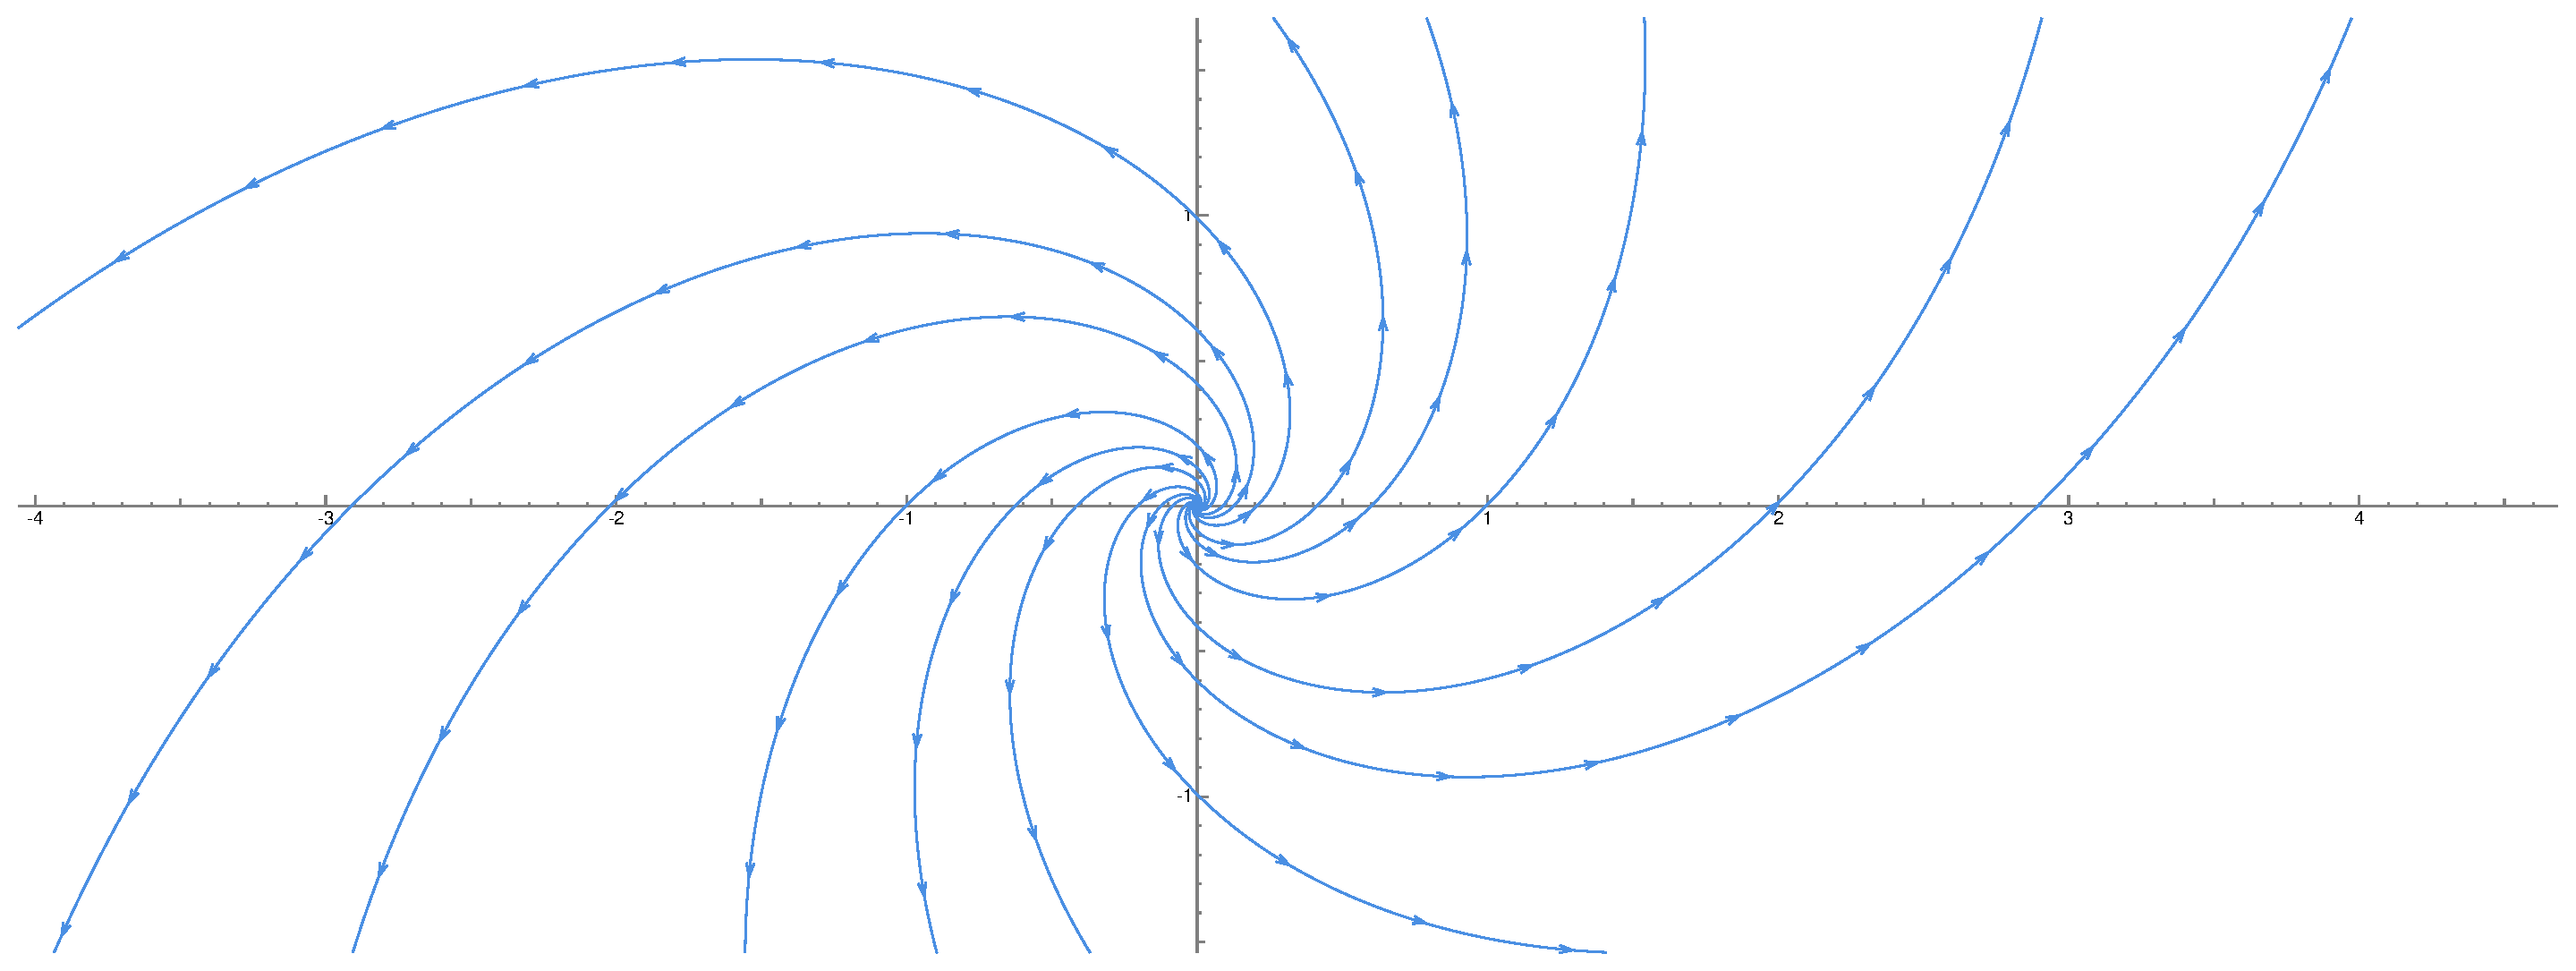
\includegraphics[width=11cm]{Immagini/fuoco_instabile.pdf}
    \caption{Fuoco instabile}
\end{figure}


\begin{figure}[!htb]
    \centering
    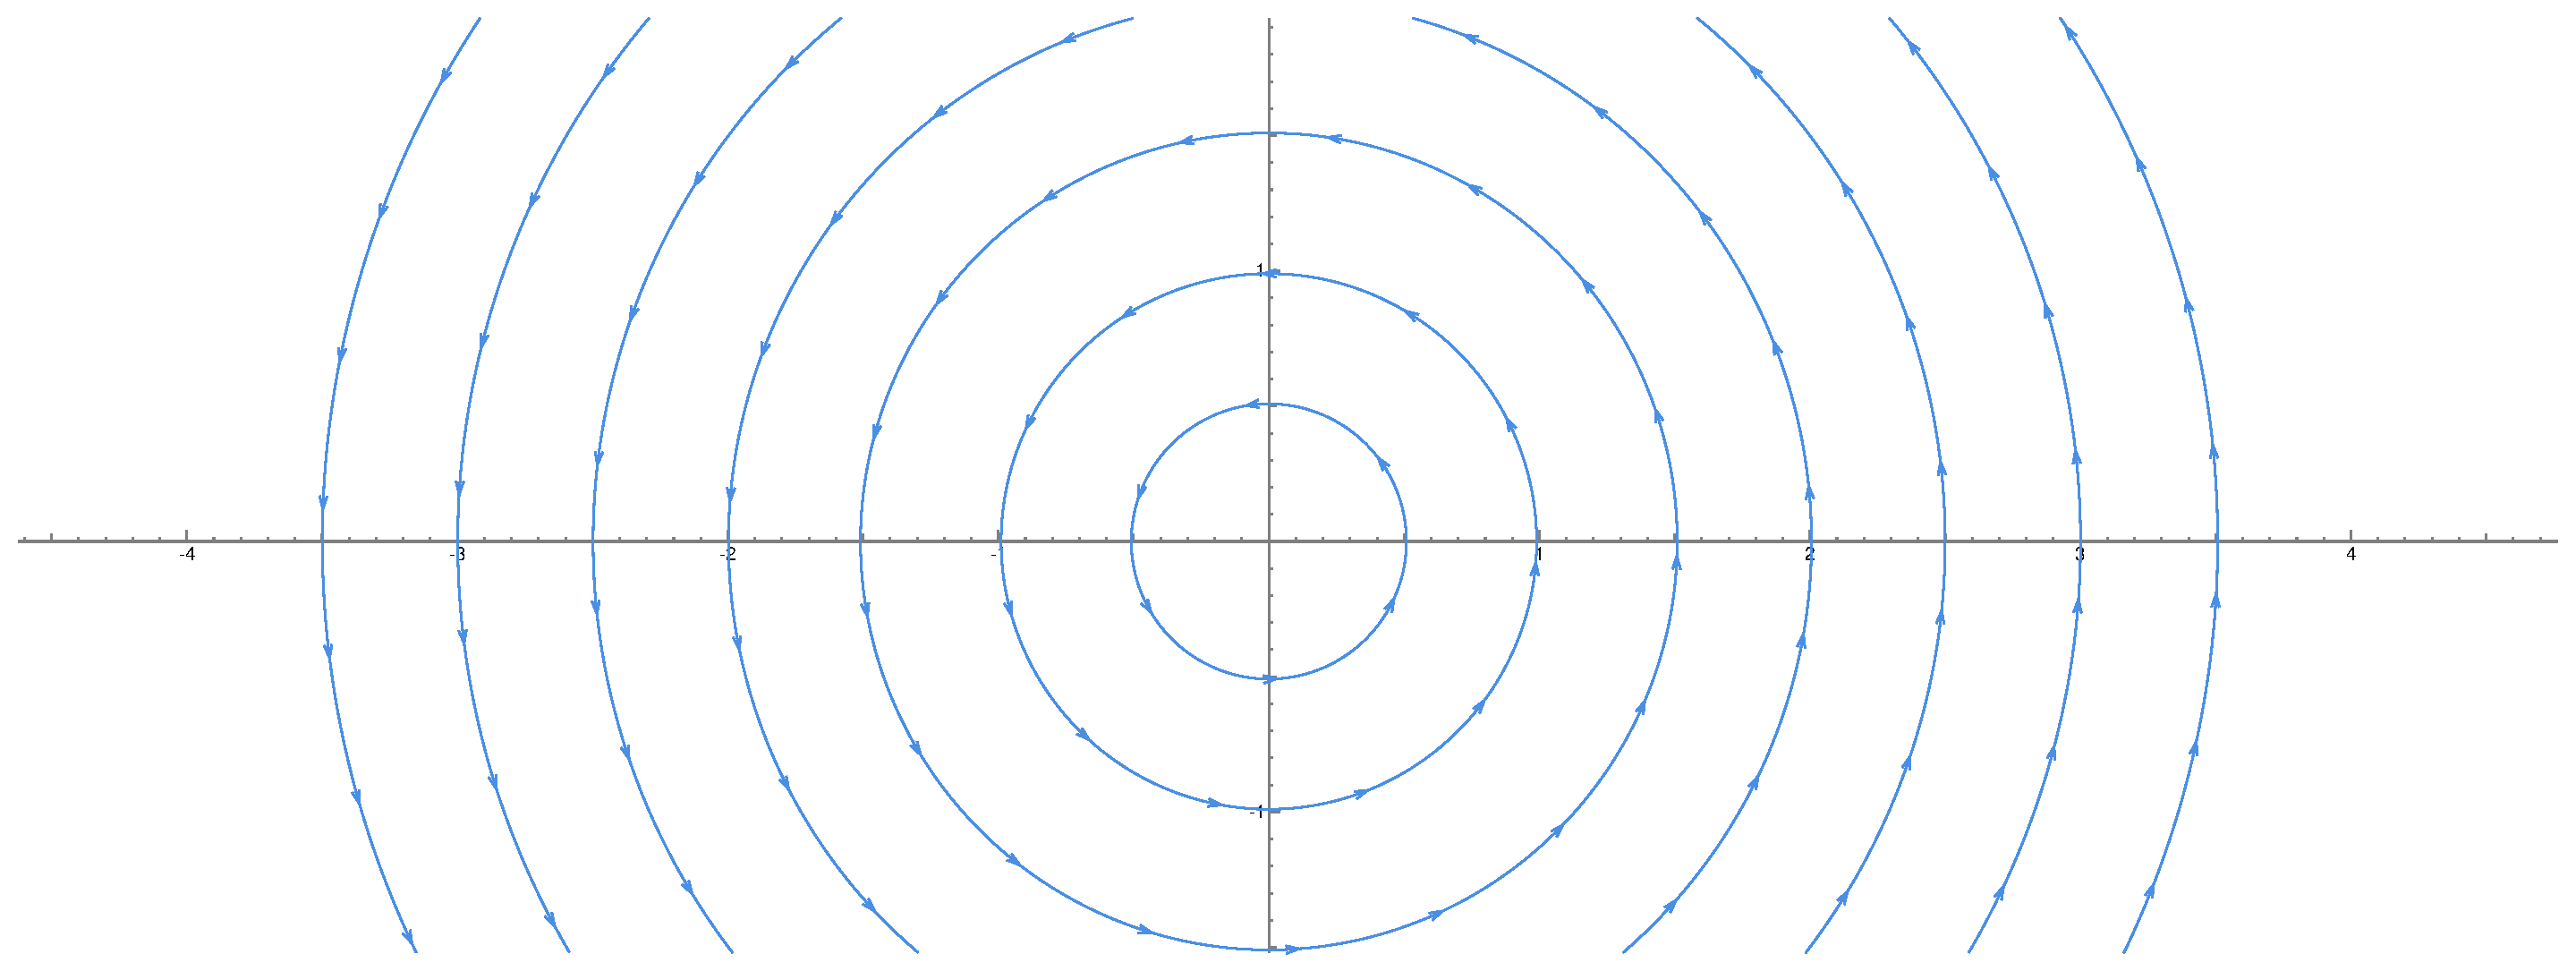
\includegraphics[width=11cm]{Immagini/centro.pdf}
    \caption{Centro}
\end{figure}


\begin{figure}[!htb]
    \centering
    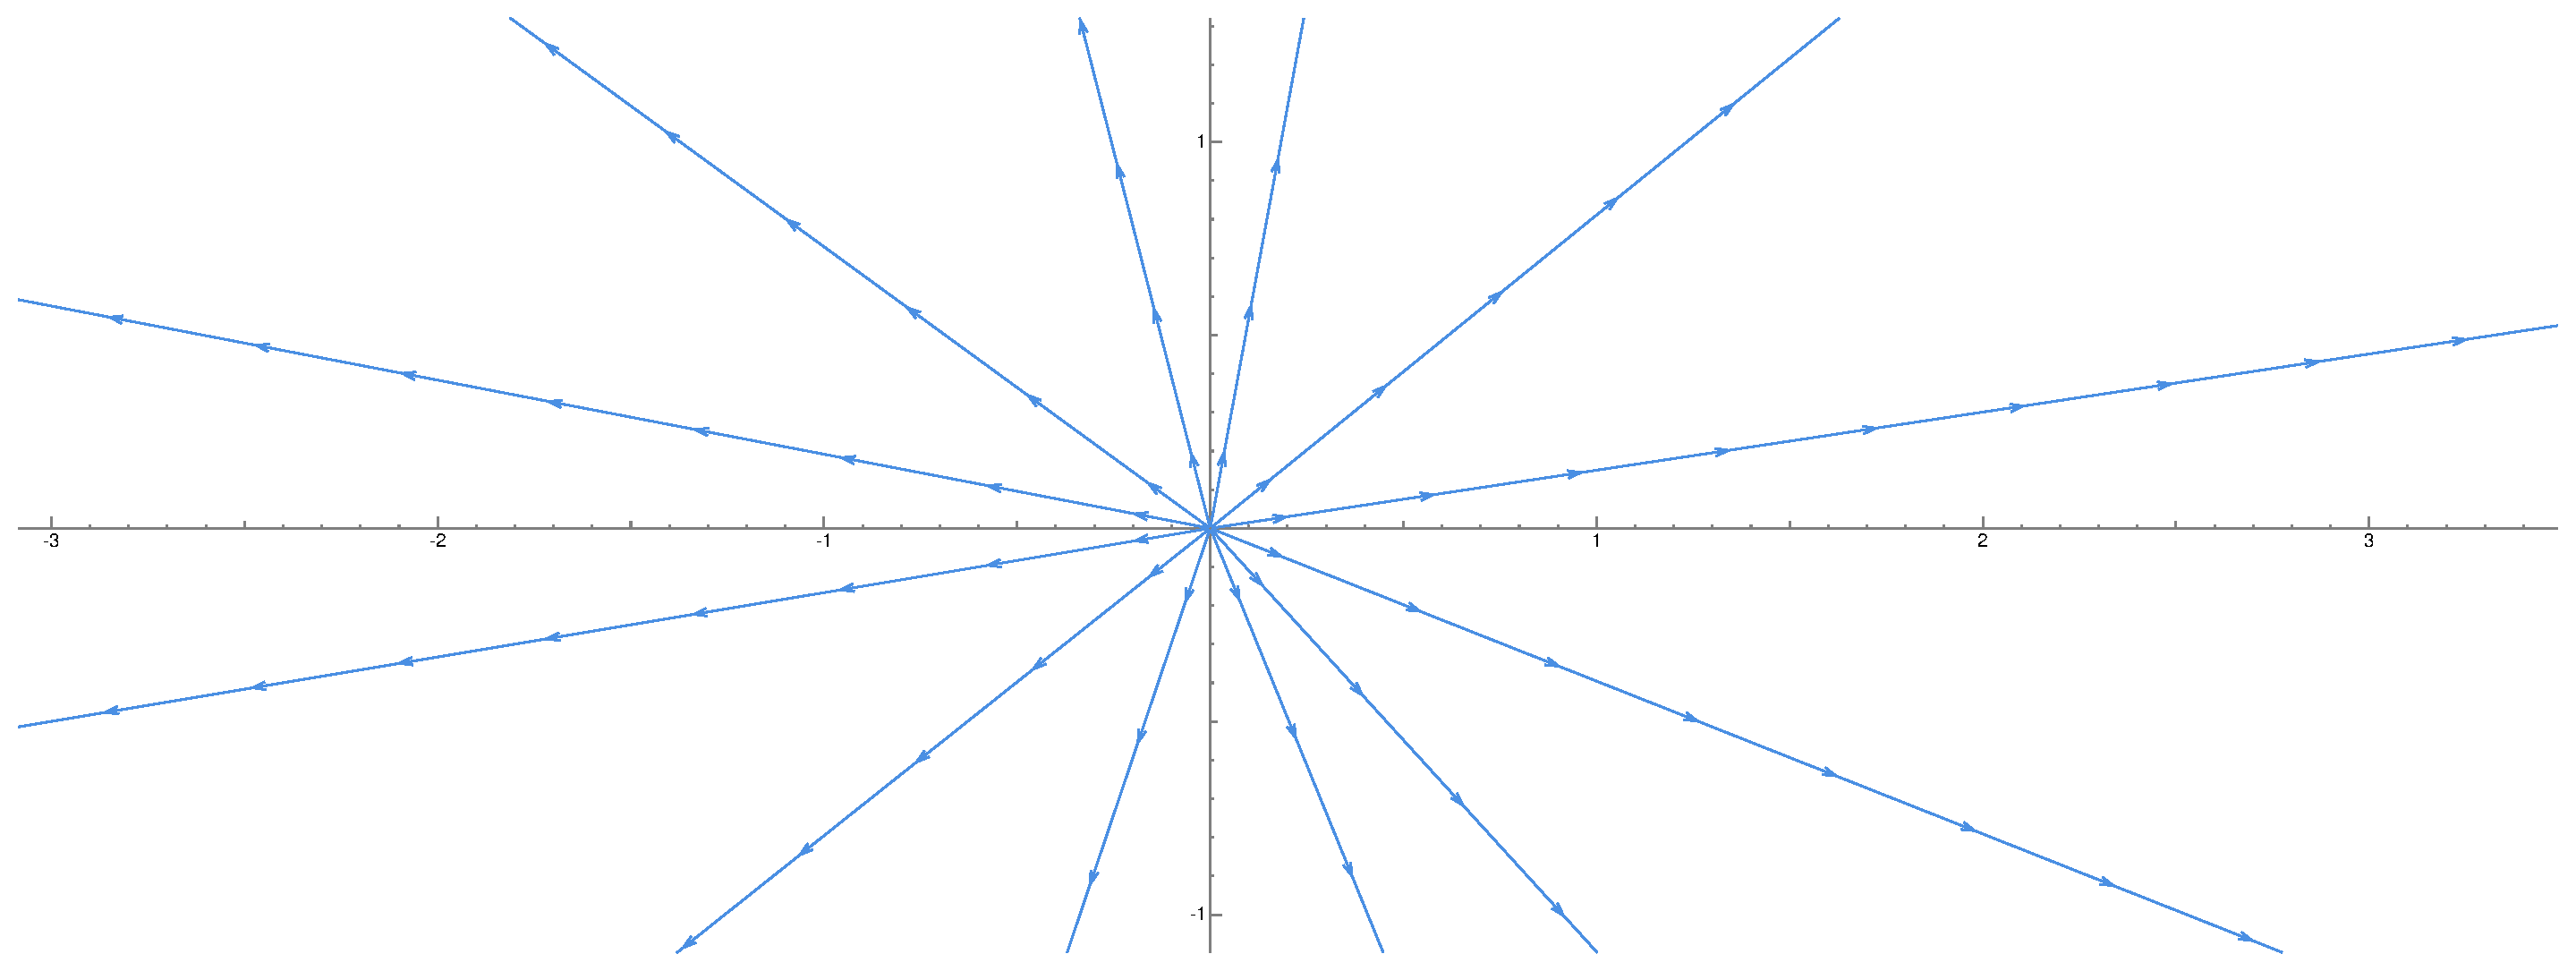
\includegraphics[width=11cm]{Immagini/stella_instabile.pdf}
    \caption{Stella instabile}
\end{figure}


\begin{figure}[!htb]
    \centering
    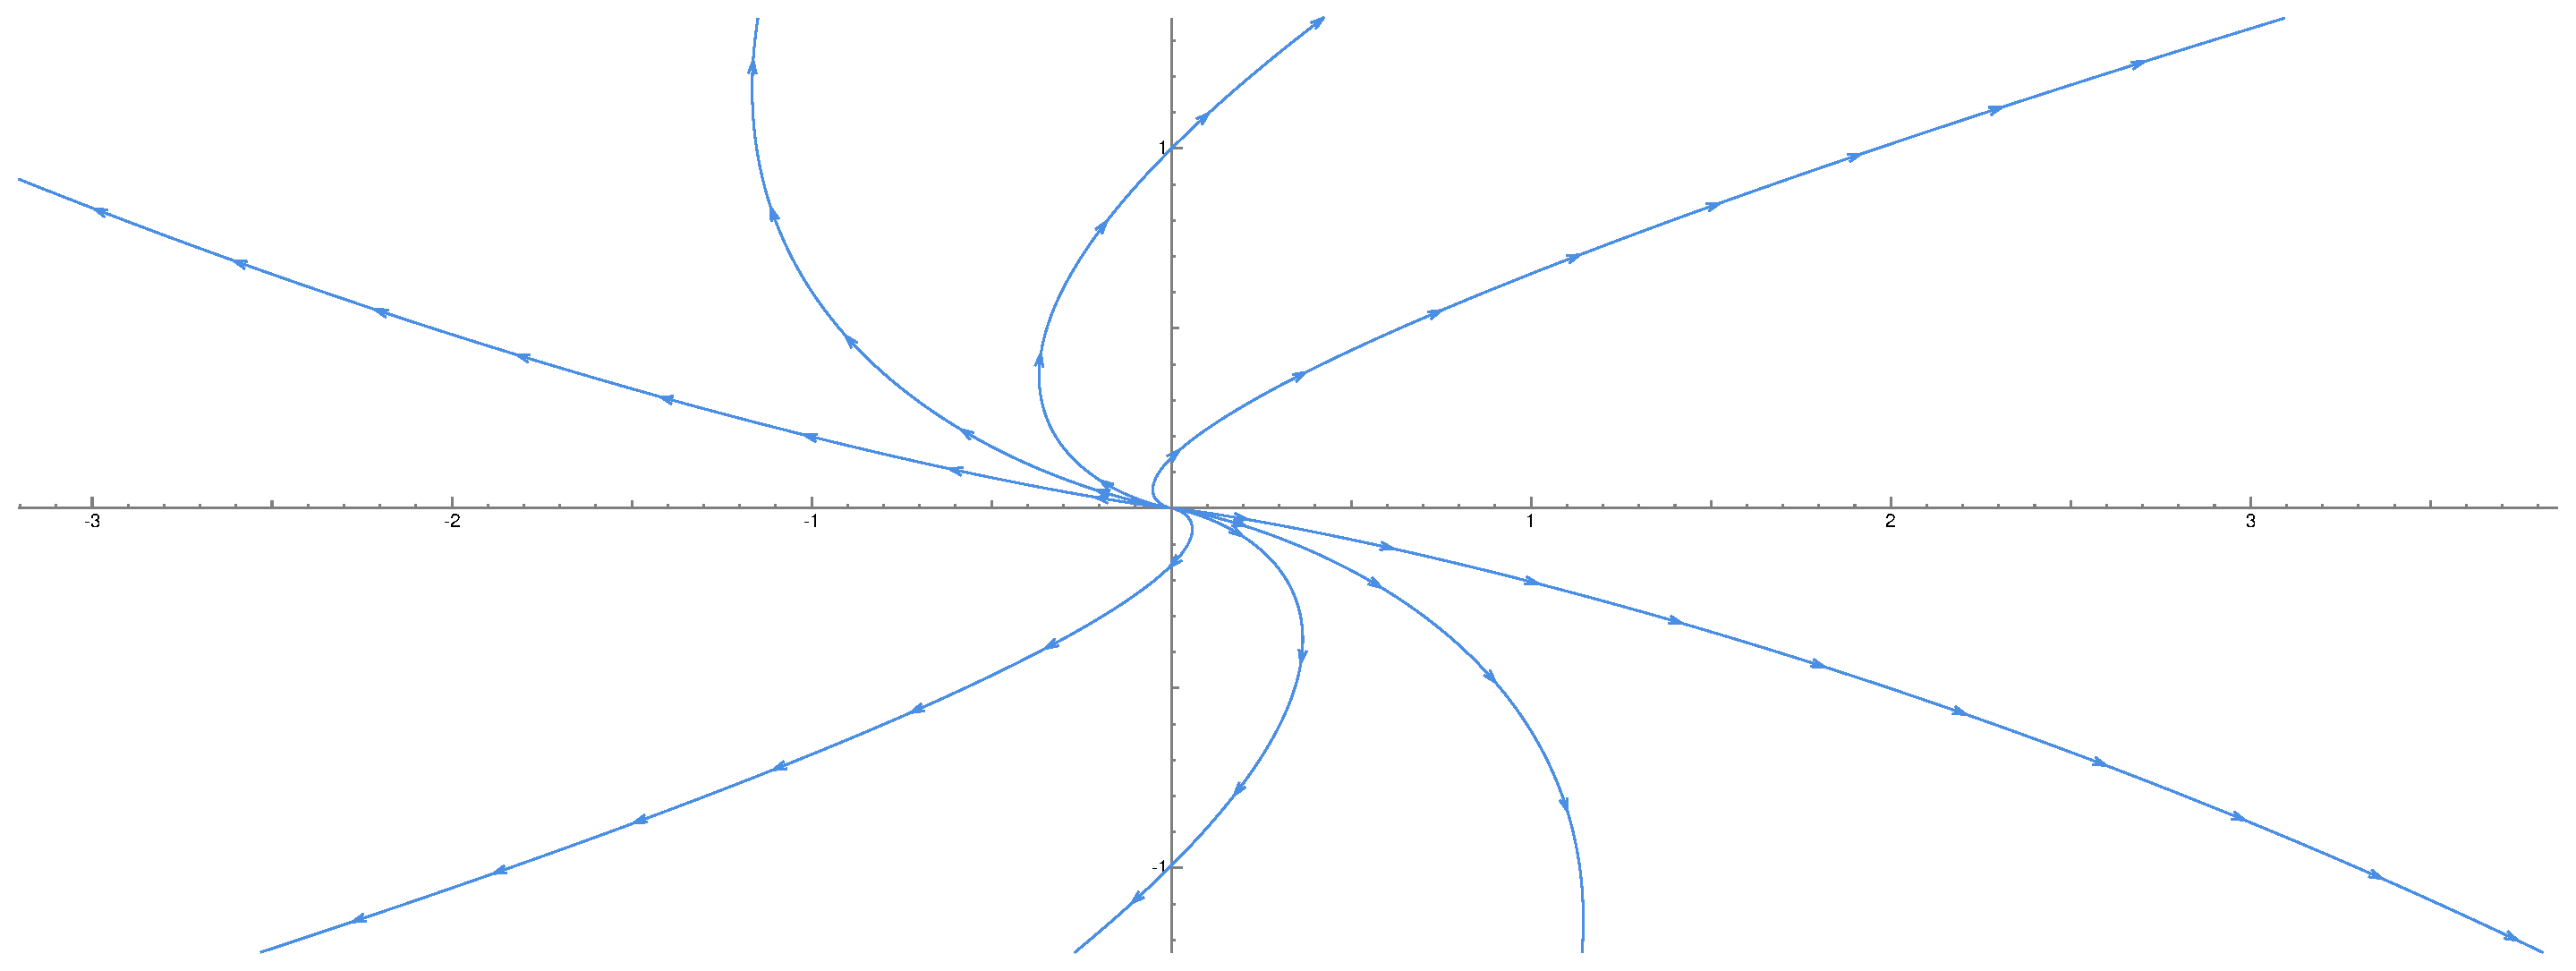
\includegraphics[width=11cm]{Immagini/nodo_improprio_instabile.pdf}
    \caption{Nodo improprio instabile}
\end{figure}


\begin{figure}[!htb]
    \centering
    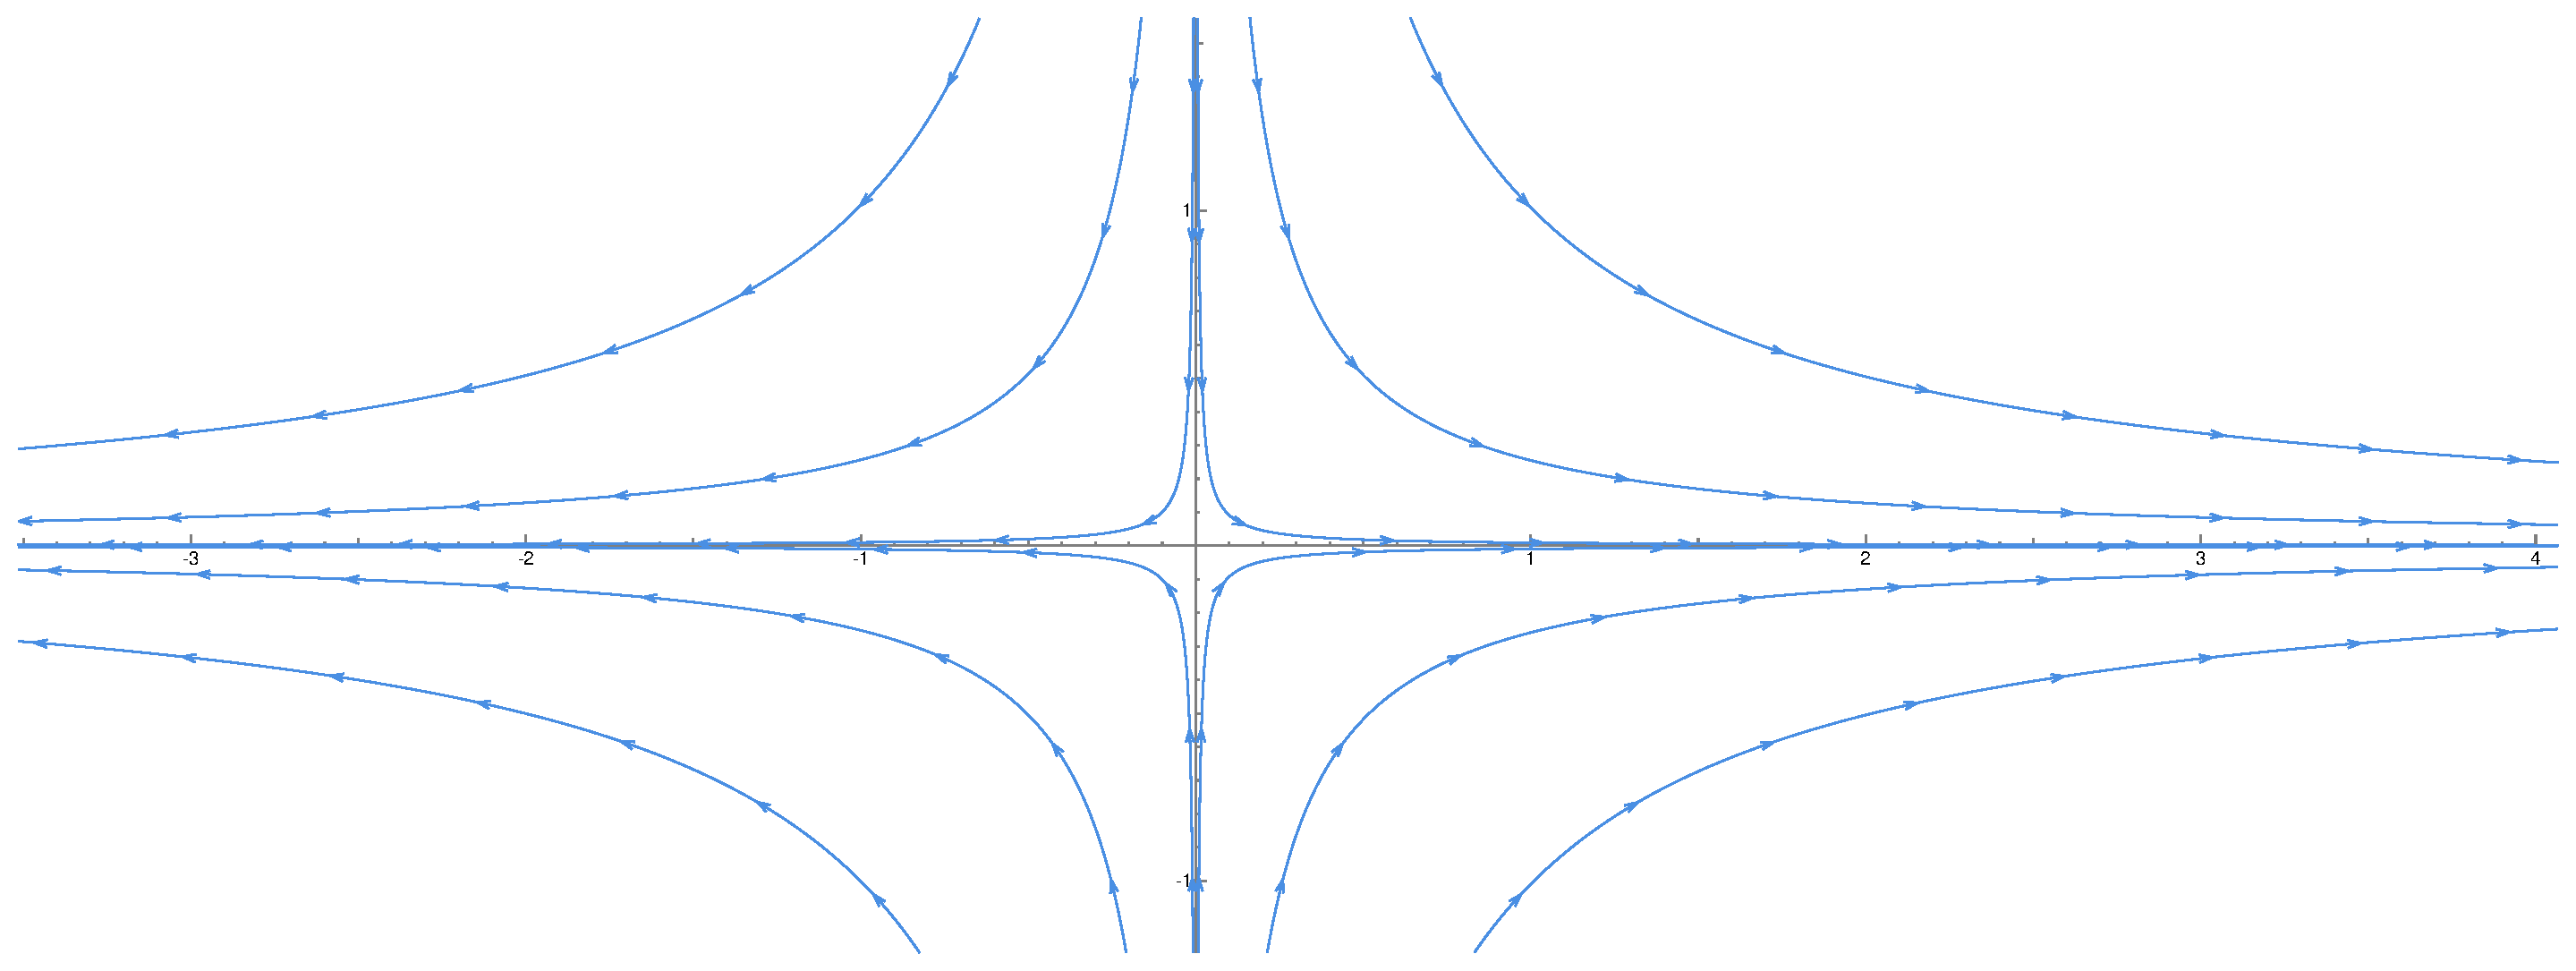
\includegraphics[width=11cm]{Immagini/sella.pdf}
    \caption{Sella}
\end{figure}


\begin{figure}[!htb]
    \centering
    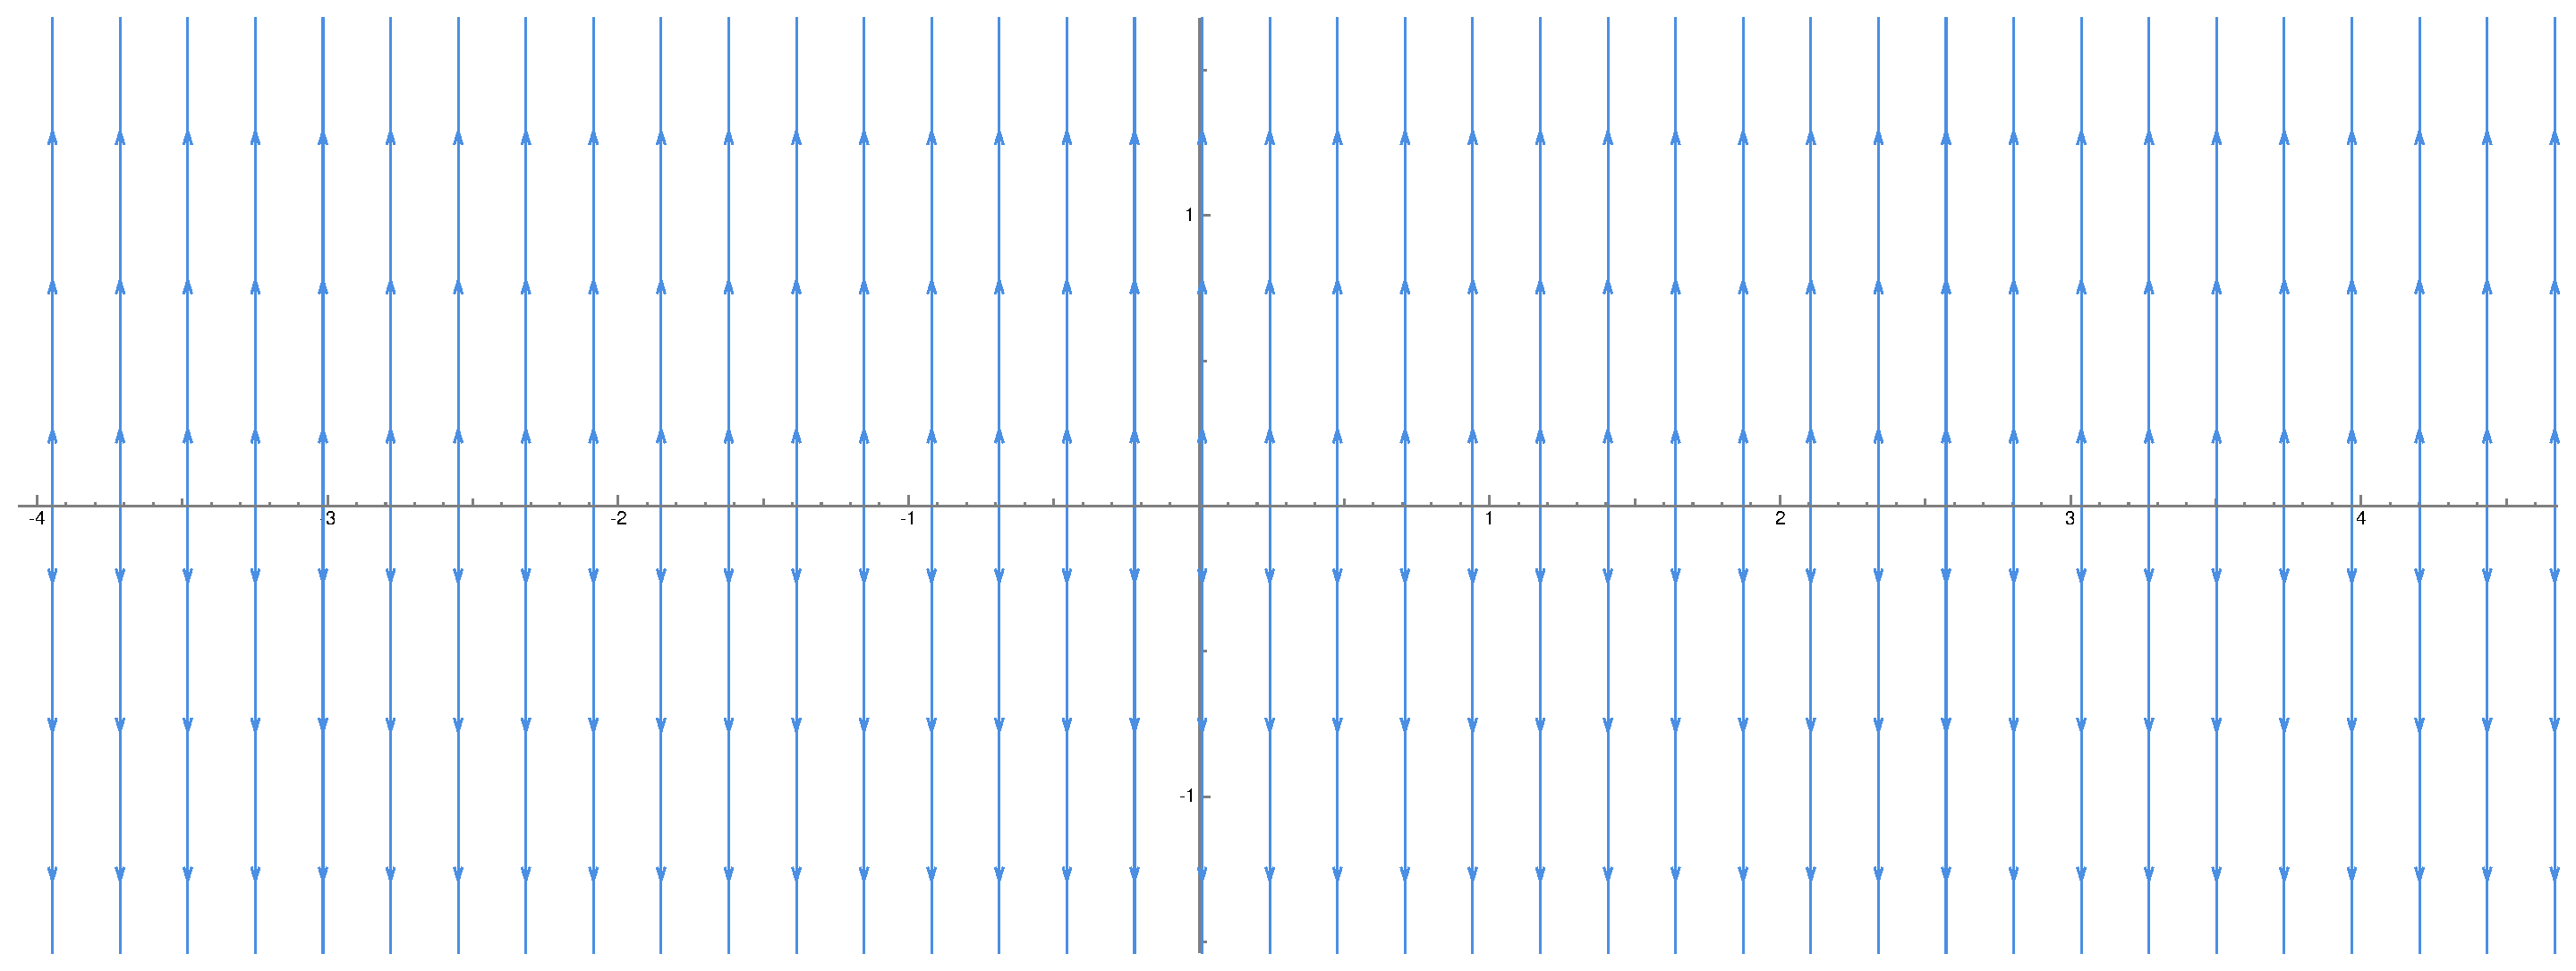
\includegraphics[width=11cm]{Immagini/rette_diagonale.pdf}
    \caption{Rette per matrice diagonalizzabile}
\end{figure}


\begin{figure}[!htb]
    \centering
    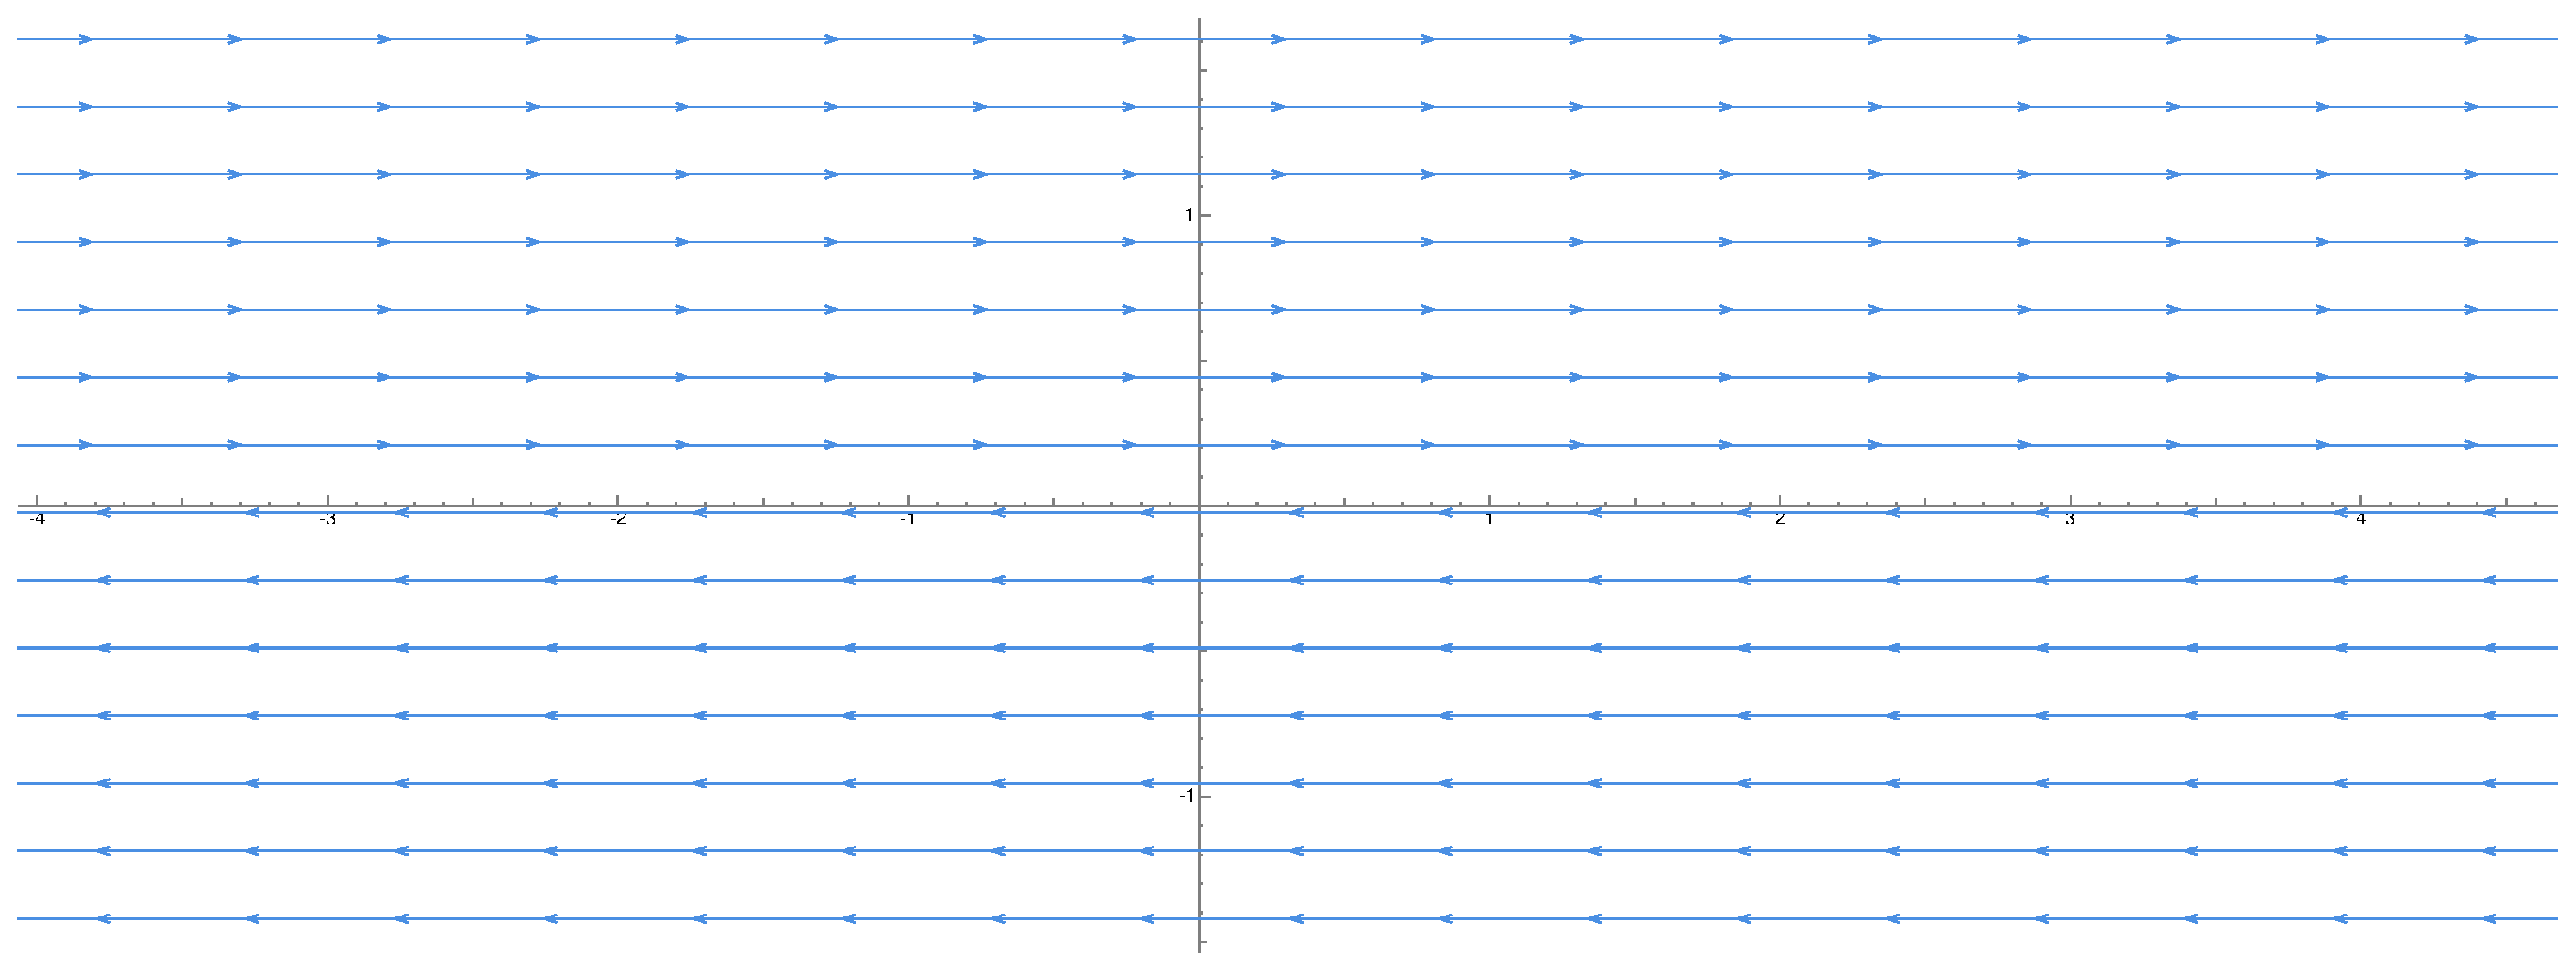
\includegraphics[width=11cm]{Immagini/rette_jordan.pdf}
    \caption{Rette per blocco di Jordan nilpotente}
\end{figure}





\chapter{Integrali Primi e Sistemi Hamiltoniani}
In questo capitolo introduciamo una classe di sistemi che ammettono integrale primo (e quindi ci permettono di fare uno studio globale guardando le curve di livello di questo). A volte, anche se un sistema non \`e della forma trattata in questo capitolo, \`e possibile studiarne il comportamento approssimandolo prima ad uno di questi e poi perturbando la soluzione trovata in modo opportuno.
\section{Sistemi Hamiltoniani}
\begin{notation}
Quando consideriamo lo spazio $\R^{2d}$ in questo capitolo indichiamo le coordinate come $(x,y)=(q,p)\in\R^{2d}$ con $x=q\in\R^d$ e $y=p\in\R^d$. In genere $q$ \`e detto \textbf{coordinata generalizzata} e $p$ \`e detto \textbf{momento generalizzato}.\\
Con la notazione $\pp xH$ intendiamo il vettore la cui componente $i$-esima \`e $\ppxi iH$. Similmente per $\pp yH$.
\end{notation}
\begin{definition}[Sistema Hamiltoniano]
Un sistema di ODE su $\R^{2d}$ \`e un \textbf{sistema Hamiltoniano} se \`e della forma
\[\mat{\dot x\\ -\dot y}=\nabla H\coimplies \begin{cases}
\displaystyle \dot x_i=\pp{y_i}H\\\\
\displaystyle \dot y_i=-\pp{x_i}H
\end{cases}\text{per ogni }i\in\cpa{1,\cdots,d},\]
dove $H:\R^{2d}\to\R$ \`e una funzione di classe $C^2(\R^{2d})$ detta \textbf{funzione Hamiltoniana} del sistema.\\
Il numero $d$ \`e detto numero di \textbf{gradi di libert\`a}.
\end{definition}
\begin{remark}
Ad ogni funzione $H:\R^{2d}\to\R$ di classe $C^2$ \`e associato un sistema Hamiltoniano.
\end{remark}

\begin{proposition}[Hamiltoniana \`e un integrale primo]\label{HamiltonianaEIntegralePrimo}
Se $H$ \`e una funzione Hamiltoniana allora \`e un integrale primo del sistema ad essa associato.
\end{proposition}
\begin{proof}
Basta calcolare $\dot H$.
\begin{align*}
\dot H(x,y)=&\nabla H(x,y)\cdot \mat{\displaystyle \pp {y}H \\\\ \displaystyle -\pp {x}H}=\\
=&\sum_{i=1}^d\pa{\pp{x_i}H\pp{y_i}H+\pp{y_i}H\pa{-\pp{x_i}H}}=0.
\end{align*}
\end{proof}

\begin{example}
Un sistema con due gradi di libert\`a \`e dato dal doppio pendolo, il quale \`e interamente determinato da due angoli. Lo spazio delle fasi \`e $T^2\times \R^2$ dove $T^2=S^1\times S^1$ parametrizza i due angoli e $\R^2$ le velocit\`a angolari.\\
Osserviamo intuitivamente che $\dim \cpa{H=c}=3$, che vedremo essere la minima dimensione che permette orbite caotiche.
\end{example}
\begin{example}[Un grado di libert\`a e mezzo]
Se un sistema ha un grado di libert\`a ma non \`e autonomo possiamo renterpretarlo come un sistema con due gradi di libert\`a dove abbiamo aggiunto il tempo e questi sistemi possono ancora presentare comportamenti caotici. Un esempio sono oscillatori armonici perturbati periodicamente.
\end{example}

\begin{theorem}[Liouville]\label{TeoremaLiouville}
Sia $H:\R^{2d}\to \R$ di classe $C^3$ e sia $\phi_t$ il flusso del sistema Hamiltoniano associato. Allora per ogni $A\subseteq \R^{2d}$ misurabile si ha che per ogni $t\in\R$
\[\Lc(A)=\Lc(\phi_t(A)).\]
\end{theorem}
\begin{proof}
Osserviamo che
\[\dd t{}\phi_t(x,y)=F(\phi_t(x,y))=\mat{\displaystyle\pp yH(\phi_t(x,y))\\\\\displaystyle-\pp xH(\phi_t(x,y))}.\]
Poich\'e $H$ \`e di classe $C^3$, si ha che $\phi:(x,y,t)\mapsto\phi_t(x,y)$ \`e di classe $C^2$ \footnote{Poich\'e $H$ \`e $C^3$ ne deriva che $F$ \`e $C^2$. Dato che $\phi'=F(\phi)$ si ha per il teorema del differenziale totale che $\phi$ \`e almeno $C^2$ in ogni entrata.}, quindi
\[\dd t{}\pa{\Dc(\phi_t(x,y))}\pasgnl={regolarit\`a}\Dc \under{=F(\phi_t(x,y))}{\pa{\dd t{}\phi_t(x,y)}}=\Dc F(\phi_t(x,y))\Dc (\phi_t(x,y)).\]
Poich\'e $\Dc\phi_0(x,y)=I$, possiamo integrare l'identit\`a precedente\footnote{\`e come se stessimo risolvendo insieme tutti i sistemi della forma \[\dd t{}{}v(t)=\Dc F(\phi_t(x,y))v(t),\quad\text{per } v(t)=\Dc(\phi_t(x,y))e_i:\R\to \R^{2d}.\]} per trovare
\[\Dc(\phi_t(x,y))=\exp\pa{\int_0^t\Dc F(\phi_s(x,y))ds}.\]
Segue da una identit\`a nota\footnote{$\det(e^A)=e^{\tr A}$} che
\begin{align*}
\det{\Dc(\phi_t(x,y))}=&\exp\pa{\int_0^t\tr\pa{\Dc F(\phi_s(x,y))}ds}.
\end{align*}
Per il teorema di Schwarz 
\[\pp{x_i\del y_i}{^2H}=\pp{y_i\del x_i}{^2H},\] 
dunque $\tr(\Dc F)=0$, da cui
\[\tr\pa{\Dc F(\phi_s(x,y))}=0.\]
Segue che
\[\det{\Dc(\phi_t(x,y))}=e^0=1.\]
Concludiamo con il seguente conto
\begin{align*}
\Lc(\phi_t(A))=&\int_{\phi_t(A)}1d\Lc=\int_A\abs{\det \Dc \phi_t(x,y)(x,y)}d\Lc=\\
=&\int_A 1d\Lc=\Lc(A).
\end{align*}
\end{proof}

\subsection{Sistemi meccanici con un grado di libert\`a}
\begin{definition}[Sistema meccanico]
Un \textbf{sistema meccanico} \`e un sistema Hamiltoniano della forma
\[H(x,y)=\frac12y^\top A y+V(x)\]
con $V:\R^d\to\R$ e $A\in Sym(d,\R)$. La funzione $V$ \`e detta \textbf{potenziale}.
\end{definition}

\noindent Studiamo un sistema meccanico con un grado di libert\`a:\\
A meno di riscalamento poniamo $A=\mat1$.
\[\begin{cases}
\displaystyle\dot x=\pp yH=y\\\\
\displaystyle\dot y=-\pp xH=-V'(x)
\end{cases}\]
Osserviamo che i punti fissi sono $\cpa{(x,0)\mid V'(x)=0}$. La matrice Jacobiana \`e data da
\[\Dc F(x,y)=\mat{0 & 1\\-V''(x) &0}\implies \tr \Dc F=0,\ \det \Dc F=V''(x).\]
Se $V''(x)=0$ siamo in un caso degenere e il linearizzato non ci aiuta.\\
Se $V''(x)<0$ il punto $(x,0)$ \`e una sella.\\
Se $V''(x)>0$ il punto $(x,0)$ \`e un punto non iperbolico di tipo centro.
\vspace*{0.5cm}

\noindent Il teorema di linearizzazione ci informa solo sul caso $(x,0)$ sella. Studiamo la stabilit\`a del caso di tipo centro.



\begin{proposition}[Caratterizzazione dei punti fissi in sistema meccanico ad un grado di libert\`a]\label{CaratterizzazionePuntiFissiSistemaMeccanico1GradoLiberta}
I punti fissi non degeneri\footnote{$(x_0,0)$ con $V'(x_0)=0$ e $V''(x_0)\neq 0$} di un sistema meccanico ad un grado di libert\`a sono selle o centri\footnote{non solo nel linearizzato}.
\end{proposition}
\begin{proof}[Idea di dimostrazione.]
Se $(x_0,0)$ fosse instabile, esisterebbe un $\e>0$ tale che per ogni $\delta>0$ esiste $z_0\in B_\delta((x_0,0))$ tale che $\norm{\phi_t(z_0)-(x_0,0)}>\e$. Poniamo
\[m_\e=\min_{\del{B_\e((x_0,0))}} H\]
e consideriamo un $\e$ abbastanza piccolo in modo tale che $m_\e\sup_{B_\e((x_0,0))} H$, che sappiamo esistere perch\'e da noti criteri sulle derivate prime e seconde $(x_0,0)$ \`e un minimo locale di $H$.
Poich\'e le orbite del sistema corrispondono alle curve di livello di $H$ abbiamo trovato una contraddizione in quanto per $\e$ abbastanza piccolo le orbite non possono attraversare $\del B_\e((x_0,0))$.\\
Se $(x_0,0)$ fosse asintoticamente stabile esisterebbe un intorno di $(x_0,0)$ che converge a $(x_0,0)$, in particolare l'area di questo intorno non si conserva, contraddicendo il teorema di liouville (\ref{TeoremaLiouville}).
\end{proof}

\chapter{Primi metodi di studio globale}
\section{Metodo delle isocline nel piano}
Supponiamo $F=(f,g)$ con $f,g:\R^2\to \R$ di classe $C^1$.

\noindent
Introduciamo un metodo che permette di calcolare esplicitamente orbite in qualche caso.
\begin{proposition}[Metodo delle isocline nel piano]\label{MetodoIsoclineNelPiano}
Sia $(x_0,y_0)$ tale che $F(x_0,y_0)\neq (0,0)$, allora esiste un intorno $U$ di $(x_0,y_0)$ tale che $\Oc(x_0,y_0)\cap U$ \`e il grafico di una funzione $h(x)$ (se $f(x_0,y_0)\neq 0$, altrimenti $h(y)$) che risolve l'equazione differenziale
\[\dd x{h(x)}=\frac{g(x,h(x))}{f(x,h(x))}.\]
\end{proposition}
\begin{proof}
Senza perdita di generalit\`a supponiamo $f(x_0,y_0)\neq 0$, esiste dunque $U$ intorno di $(x_0,y_0)$ dove $f$ non si annulla. Consideriamo la funzione
\[I(x,y)=y-h(x)\]
dove $h(x)$ \`e la soluzione del problema di Cauchy 
\[\dd x{h(x)}=\frac{g(x,h(x))}{f(x,h(x))},\quad h(x_0)=y_0\] 
definita in un intorno di $x_0$ contenuto nella proiezione sulla prima componente di $U$. Osserviamo che
\[\dot I\res{I=0}(x,y)=\dot y-h'(x)\dot x\res{I=0}=\rbar{g(x,y)-\frac{g(x,h(x))}{f(x,h(x))}f(x,y)}_{y=h(x)}=0,\]
dunque per il criterio (\ref{CostruzioneInsiemiInvariantiCurveDiLivello}) sappiamo che $\cpa{y=h(x)}$ \`e un insieme invariante. Poich\'e \`e una curva e contiene $(x_0,y_0)$ questa \`e l'orbita voluta ed effettivamente l'abbiamo scritta come grafico.
\end{proof}

\section{Ricerca di simmetrie}
Spesso, soprattutto negli esercizi, i sistemi in esame presentano delle simmetrie, ovvero \`e possibile costruire una mappa\footnote{Durante il corso non \`e stata data una definizione rigorosa di simmetria, solo una idea intuitiva e pratica di come impiegarla nella risoluzione di esercizi. Questa formulazione NON \`e stata data durante il corso e non so se \`e standard, serve solo some guida per capire il concetto a chi legge le dispense.}
\[\funcDef{C^1(\R,\R^d)}{C^1(\R,\R^d)}{x(t)}{\wt x(t)}\]
tale che 
\[\dd t{}x(t)=F(x(t))\implies \dd t{}\wt x(t)=F(\wt x(t)).\]
Spesso una simmetria si fattorizza in una mappa ``geometrica" composta con una mappa ``temporale", cio\`e esistono $\tau:\R\to \R$ e $g:\R^d\to\R^d$ tali che
\[\wt x(t)=g(x(\tau(t))).\]

\begin{example}[Esempio di simmetrie]
Consideriamo il sistema
\[\begin{cases}
\dot x=x^2\\
\dot y=y^2
\end{cases}\]
L'unico punto fisso \`e $(0,0)$ e gli assi sono invarianti. Ci sono altre rette invarianti? Cio\`e, esistono $a,b$ tali che una curva di livello di $I(x,y)=ax+by$ \`e invariante?
\begin{align*}
\dot I\res{I=c}=&a\dot x+b\dot y\res{ax+by=c}\pasgnl={se $b\neq 0$}\\
=&ax^2+by^2\res{ax+by=c}=ax^2+b\pa{\frac{c-ax}b}^2=\\
=&\pa{a+\frac{a^2}b}x^2-2\frac{ac}bx+\frac{c^2}b.
\end{align*}
Per annullare tutti i coefficienti $c=0$ e $a\in\cpa{0,-b}$. Troviamo dunque le condizioni $c=0$ e $a=0$ o $a=-b$. Dunque $\cpa{x=y}$ \`e un insieme invariante.
    
Andiamo ora a studiare le isocline. Per $x\neq 0$ consideriamo
\[\dd yx=\frac{y^2}{x^2}\implies -\frac1{y(x)}+\frac1{y_0}=-\frac1x+\frac1{x_0}\implies y(x)=\dfrac1{\frac1x+\pa{\frac1{y_0}-\frac1{x_0}}}.\]
Studiamo le simmetrie del sistema. Proviamo a porre $(\wt x(t),\wt y(t))=(-x(-t),-y(-t))$, da cui
\[\dd t{} \wt x(t)=-\dot x(-t)(-1)=\dot x(-t)=x^2(-t)=(-\wt x(t))^2=(\wt x(t))^2\]
e similmente per $\wt y$. Questo mostra che ad ogni orbita possiamo associarne un'altra che geometricamente \`e la riflessione rispetto all'origine e che viene percorsa in verso opposto.
\end{example}
\chapter{Variet\`a stabili/instabili}

\section{Variet\`a stabili e instabili locali}
In un punto fisso lineare di tipo sella sappiamo che esistono due assi: uno che converge al punto ($E^s$) e uno che vi diverge ($E^u$).\\
Cerchiamo di generalizzare questo concetto.

\begin{definition}[Variet\`a stabile/instabile locale]
Siano $x_0$ un punto fisso iperbolico per $\dot x=F(x)$ e $U$ un intorno di $x_0$. La \textbf{variet\`a stabile locale} di $x_0$ in $U$ \`e data da
\[W^s_{loc}(x_0)=\cpa{y\in U\mid \forall t\geq 0\ \phi_t(y)\in U,\ \lim_{t\to+\infty}\phi_t(y)\to x_0}.\]
Similmente definiamo la \textbf{variet\`a instabile locale} come
\[W^{u}_{loc}(x_0)=\cpa{y\in U\mid \forall t\leq 0\ \phi_t(y)\in U,\ \lim_{t\to-\infty}\phi_t(y)\to x_0}.\]
\end{definition}


\begin{theorem}[Variet\`a stabile/instabile]\label{TeoremaVarietaStabileInstabile}
Sia $x_0$ un punto fisso iperbolico\footnote{ricordiamo che $x_0$ iperbolico implica in particolare che $\dim E^s(x_0)+\dim E^u(x_0)=d$, dove $\R^d$ \`e lo spazio delle fasi.} per $F\in C^k$ e $k\geq 1$. Allora esiste $\e>0$ tale che
\setlength{\leftmargini}{0.5cm}
\begin{enumerate}
\item $W_{loc}^{s/u}(x_0)$ in $B_\e(x_0)$ esistono e sono uniche,
\item $W^s_{loc}(x_0)$ \`e positivamente invariante e $W^u_{loc}(x_0)$ \`e negativamente invariante,
\item $W^{s/u}_{loc}(x_0)$ sono sottovariet\`a di $B_\e(x_0)$ di classe $C^k$.\\
Inoltre $\dim W^s_{loc}(x_0)=\dim E^s(x_0)$ e $\dim W^u_{loc}(x_0)=\dim E^u(x_0)$.
\item I sottospazi affini $x_0+E^{s/u}(x_0)$ sono tangenti a $W^{s/u}_{loc}$ in $x_0$.
\end{enumerate}
\end{theorem}
\begin{proof}[Dimostrazione. (Caso $d=2$)]
Poich\'e $x_0$ \`e un punto fisso iperbolico si presentano due casi: le parti reali dei due autovalori hanno lo stesso segno o hanno segno opposto. Se hanno lo stesso segno sappiamo che $\det \Dc F(x_0)>0$ e che $\tr \Dc F(x_0)\neq 0$. Segue dunque che $W^s_{loc}(x_0)=B_\e(x_0)$ e $W^u_{loc}(x_0)=\cpa{x_0}$ o viceversa a seconda del segno delle parti reali. Da queste caratterizzazioni \`e evidente che il teorema vale.
\vspace{0.5cm}

\noindent Supponiamo dunque che le parti reali dei due autovalori abbiano segno opposto. Segue immediatamente che $x_0$ \`e un punto di sella e che gli autovalori sono reali. Siano $-\la$ e $\mu$ questi autovalori (dove $\la,\mu>0$). A meno di una traslazione e un cambio base supponiamo
\[x_0=(0,0),\ \Dc F(x_0)e_1=-\la e_1,\quad \Dc F(x_0)e_2=\mu e_2.\]
Possiamo dunque riscrivere il sistema come
\[\begin{cases}
\dot x=-\la x+f(x,y)\\
\dot y=\mu y+g(x,y)
\end{cases}\]
dove $f,g$ sono di classe $C^k$, $f(0,0)=g(0,0)=0$\footnote{in quanto $x_0=(0,0)$ \`e un punto fisso}, $\nabla f(0,0)=\nabla g(0,0)=(0\ 0)^\top$\footnote{in quanto sappiamo che $\Dc F((0,0))=\pa{\smat{-\la &0\\0&\mu}}$} e le seguenti funzioni sono $o$-piccoli di $\sqrt{x^2+y^2}$: $f,\ g,\ \pp xf,\ \pp yf,\ \pp xg$ e $\pp y g$\footnote{per come funziona l'espansione di Taylor}.\\
Data questa trasformazione, la tesi \`e equivalente a mostrare che $W^s_{loc}(0,0)$ esiste, \`e unico, positivamente invariante, di classe $C^k$ e tangente a \[\cpa{y=0}=(0,0)+E^s((0,0))\text{ in }(0,0).\] Un argomento simmetrico mostra i risultati mancanti relativi a $W^u_{loc}$.
\vspace{0.5cm}

\noindent Definiamo i seguenti insiemi: per ogni $\e>0$ e per ogni $M>1$ siano
\[D_\e=\cpa{|x|\leq\e,\ |y|\leq \e},\ C_M=\cpa{|x|\geq M|y|},\ C_M^+=C_M\cap\cpa{x>0}\cap D_\e,\]
\begin{align*}
I^+_\e=&\cpa{y\in(-\e,\e)\mid (\e,y)\in C_M,\ \exists t_0>0\ t.c.\ \phi_{t_0}(\e,y)\in \del C_M^+\cap \cpa{y>0}}\\
I^-_\e=&\cpa{y\in(-\e,\e)\mid (\e,y)\in C_M,\ \exists t_0>0\ t.c.\ \phi_{t_0}(\e,y)\in \del C_M^+\cap \cpa{y<0}}.
\end{align*}
La dimostrazione si articola nei seguenti passi:
\begin{itemize}
\item Per $\e$ abbastanza piccolo, $\dot x$ \`e negativo su $C^+_M$
\item Per $\e$ abbastanza piccolo, $\dot y$ ha lo stesso segno di $y$ sul bordo $\del C^+_M$
\item Gli insiemi $I^+_\e$ e $I^-_\e$ sono (intervalli) aperti
\item Per ogni $(\e,y)\in C_M$ sappiamo che $\Oc^+(\e,y)$ esce dal bordo superiore ($y\in I^+_\e$), inferiore ($y\in I^-_\e$), o converge a $(0,0)$ ($y\in (-\e,\e)\bs(I^+_\e\cup I^-_\e)$).\\
Mostriamo che esiste un solo punto $\ol y\in (-\e,\e)$ tale che $\omega((\e,\ol y))=\cpa{(0,0)}$.
\item Con il metodo delle isocline interpretiamo $\Oc^+((\e,\ol y))$ come il grafico di una funzione $h\in C^k((0,\e))$
\item Per arbitrariet\`a di $M>1$ possiamo passare al limite in $M\to+\infty$ per mostrare $h'(0)=0$, da cui segue la tangenza.
\end{itemize}
Fissiamo $M>1$ e procediamo a mostrare i primi quattro punti:
\begin{itemize}
\item[\ul{Claim}:] Esiste un $\e>0$ tale che $\dot x\res{C_M^+}<0$.
\begin{proof}[Dimostrazione del Claim.]
Ricordiamo che
\[\dot x=-\la x+f(x,y)\quad\text{con }|f(x,y)|=o(\sqrt{x^2+y^2}),\]
in particolare esiste $\e>0$ tale che per ogni $(x,y)\in D_\e$
\[\abs{f(x,y)}\leq \frac\la{2\sqrt 2}\sqrt{x^2+y^2}.\]
Se $(x,y)\in C_M$ allora
\[\sqrt{x^2+y^2}\leq \sqrt{x^2\pa{1+\frac1{M^2}}}\pasgnlmath\leq{M\geq 1} \sqrt 2|x|.\]
Mettendo insieme questi risultati
\begin{align*}
\dot x\res{C_M^+}=&-\la x+f(x,y)\res{C_M^+}\leq\\
\leq& -\la x+\frac\la{2\sqrt 2}\sqrt{x^2+y^2}\res{C_M^+}\leq\\
\pasgnlmath\leq{x>0} & -\la x+\frac\la2x=-\frac\la2 x<0.
\end{align*}
\end{proof}
\item[\ul{Claim}:] Esiste un $\e>0$ tale che $\dot y\res{\del C_M^+\cap \cpa{y>0}}>0$ e $\dot y\res{\del C_M^+\cap \cpa{y<0}}<0$.
\begin{proof}[Dimostrazione del Claim.]
Ricordiamo che
\[\dot y=\mu y+g(x,y)\quad\text{con }|g(x,y)|=o(\sqrt{x^2+y^2}),\]
in particolare esiste $\e>0$ tale che per ogni $(x,y)\in D_\e$
\[\abs{g(x,y)}\leq \frac\mu{2\sqrt{1+M^2}}\sqrt{x^2+y^2}.\]
Segue che
\begin{align*}
\dot y\res{\del C_M^+\cap \cpa{y>0}}=&\mu y+g(My,y)\geq\\
\geq&\mu y-\frac\mu{2\sqrt{1+M^2}}\sqrt{(1+M^2)}y=\\
=&\frac\mu2y>0.
\end{align*}
Gli stessi conti con le disuguaglianze nel senso opposto danno la dimostrazione per $\dot y\res{\del C_M^+\cap \cpa{y<0}}$.
\end{proof}
\item[\ul{Claim}:] Gli insiemi $I_\e^+$ e $I_\e^-$ sono intervalli aperti.
\begin{proof}[Dimostrazione del Claim.]
Mostriamo la tesi solo per $I_\e^+$. Il caso $I_\e^-$ \`e simmetrico.
\setlength{\leftmargini}{0cm}
\begin{itemize}
\item[$\boxed{\text{aperto}}$] Sia $y_0\in I_\e^+$ e sia $t_0>0$ tale che $\phi_{t_0}(\e,y_0)\in \del C_M^+\cap\cpa{y>0}$. Se $\phi_t(a,b)=(x(t,a,b),y(t,a,b))$ osserviamo che $y(t_0,\e,y_0)>0$ e $x(t_0,\e,y_0)-My(t_0,\e,y_0)=0$. Definiamo
\[G(b,t)=x(t,\e,b)-My(t,\e,b).\]
Per quanto detto $G(y_0,t_0)=0$ e, per $\e>0$ abbastanza piccolo, $\dd t{}G(y_0,t_0)=\dot x(t_0,\e,y_0)-M\dot y(t_0,\e,y_0)<0\neq 0$\footnote{stiamo usando i due lemma precedenti.}.\\
Abbiamo verificato le ipotesi del teorema della funzione implicita, dunque esistono $U$ intorno di $y_0$, $V$ intorno di $t_0$ e $\tau:U\to V$ continua $C^k$ (regolarit\`a di $G$) tali che $\tau(y_0)=t_0$ e per ogni $y\in U$ abbiamo
\[G(y,\tau(y))=0\coimplies \phi_{\tau(y)}(\e,y)\in \del C_M^+.\]
La tesi segue a meno di restringere $U$ a $U\cap (\phi_{\tau(\cdot)}(\e,\cdot))\ii(\cpa{y>0})$.
\item[$\boxed{\text{connesso}}$] Segue immediatamente da esistenza e unicit\`a unito alla monotonia di $x$ in $t$ e per $\e$ abbastanza piccolo (in modo che $D_\e$ contenga come unico punto fisso $(0,0)$). 
\end{itemize}
\setlength{\leftmargini}{0.5cm}
\end{proof}
\item[\ul{Claim}:] Si ha che
\[\#\cpa{y\in(-\e,\e)\mid (\e,y)\in C_M,\ \omega(\e,y)=\cpa{(0,0)}}=1.\]
\begin{proof}[Dimostrazione del Claim.]
Supponiamo per assurdo che esistano $y_0$ e $y_1$ distinti nell'insieme. A meno di moltiplicare $F$ per una funzione scalare\footnote{\`e noto da analisi 2 che questa operazione non cambia le orbite del sistema} possiamo supporre
\[\begin{cases}
\dot x=-x\\
\displaystyle\dot y=\frac{\mu y+g(x,y)}{\la-\frac1xf(x,y)}
\end{cases}\]
A meno di conti possiamo definire $\wt \la>0$ e $\wt g$ con le stesse propriet\`a di $g$ come $o$-piccolo di $\sqrt{x^2+y^2}$ in modo tale che il sistema diventi
\[\begin{cases}
\dot x=-x\\
\dot y=\wt \la y+\wt g(x,y)
\end{cases}\]
In questo nuovo sistema $\phi_t(\e,y)=(\e e^{-t},y(t,\e,y))$, cio\`e orbite che partono con la stessa componente $x$ mantengono la stessa componente $x$. Consideriamo come cambia la distanza tra $y_0$ e $y_1$ seguendo le orbite:
\[\dd t{}\pa{y_1(t)-y_0(t)}=\dot y_1(t)-\dot y_0(t)=\wt \la(y_1(t)-y_0(t))+\wt g(\e e^{-t},y_1(t))-\wt g(\e e^{-t},y_0(t)).\]
Per il teorema di Lagrange
\[\abs{\wt g(\e e^{-t},y_1(t))-\wt g(\e e^{-t},y_0(t))}= \pp y{\wt g}(\e e^{-t},\xi(t))\abs{y_1(t)-y_0(t)}\]
con $\xi(t)\in (y_0(t),y_1(t))$. 
Sia ora $\e>0$ tale che per ogni $(x,y)\in D_\e$
\[\abs{\pp y{\wt g}}\leq \frac{\wt \la}2\sqrt{x^2+y^2}.\]
Si ha dunque che
\begin{align*}
\dd t{}\pa{y_1(t)-y_0(t)}\geq& \wt \la(y_1(t)-y_0(t))-\frac{\wt \la}2\sqrt{\e^2e^{-2t}+\xi(t)^2}\abs{y_1(t)-y_0(t)}\pasgnlmath\geq{y_1(t),y_2(t)\in D_\e}\\
\geq& \wt \la(y_1(t)-y_0(t))-\frac{\wt \la}2\e \sqrt 2 (y_1(t)-y_0(t))=\\
=&\under{>0\text{ per }\e\in(0,\sqrt 2)}{\pa{\wt \la-\frac{\wt \la}2\e\sqrt 2}}(y_1(t)-y_0(t))>0,
\end{align*}
dunque $y_1(t)-y_0(t)$ cresce, in particolare non possono entrambe convergere verso $(0,0)$.
\end{proof}
\end{itemize}
\noindent Siamo pronti per mostrare gli ultimi due punti e concludere la dimostrazione.
\smallskip

\noindent
Sia $\ol y\in(-\e,\e)$ l'unica condizione iniziale tale che $(\e,\ol y)\in C_M$ e $\omega(\e,\ol y)=(0,0)$. Si ha dunque che 
\[W^s_{loc}(0,0)\cap \cpa{x>0}=\Oc^+(\e,\ol y).\]
Ripetendo quanto fatto per $\cpa{x<0}$ troviamo l'esistenza e unicit\`a di $W^s_{loc}$.
\vspace{0.5cm}

\noindent Sappiamo che $W^s_{loc}(0,0)\cap \cpa{x>0}=\Oc^+(\e,\ol y)$ e per il metodo delle isocline (\ref{MetodoIsoclineNelPiano}) sappiamo che
\[\Oc^+(\e,\ol y)\subseteq \cpa{y=h(x)}\]
con $h(x)$ soluzione di
\[\dd xy=\frac{\mu y+g(x,y)}{-\la x+f(x,y)}.\]
Per la regolarit\`a delle funzioni che definiscono $h$ sappiamo che $h$ \`e $C^k$, quindi effettivamente $W^s_{loc}\cap \cpa{x>0}$ \`e una variet\`a $C^k$.\\
Osserviamo inoltre che $h'(0)=0$, infatti
\[\abs{h'(x)}\sim_{x\to 0^+}\abs{-\frac \mu\la\frac yx}\leq \frac\mu\la\frac1M\]
per ogni $M>1$, dunque passando al limite per $M\to+\infty$\footnote{anche se a priori per $M$ diversi dovremmo considerare $\e$, $\ol y$ e $h$ diversi, per l'unicit\`a mostrata stiamo solo restringendo il tratto di $h$ che stiamo considerando senza alterarne la forma.} troviamo $h'(0)=0$. Questo mostra la tangenza di $W^s_{loc}\cap \cpa{x>0}$ a $\cpa{y=0}$ in $(0,0)$. Ripetendo questi passaggi per l'altro semipiano troviamo finalmente la tesi. 
\end{proof}

\section{Variet\`a stabili e instabili}

\begin{definition}[Variet\`a stabile/instabile globale]
Definiamo le \textbf{variet\`a stabile/instabile globale} di $x_0$ come
\begin{align*}
W^s(x_0)=&\bigcup_{t\leq0}\phi_t\pa{W^s_{loc}(x_0)}\\
W^u(x_0)=&\bigcup_{t\geq0}\phi_t\pa{W^u_{loc}(x_0)}
\end{align*}
\end{definition}
\begin{remark}
Studiamo velocemente come $W^s$ e $W^u$ possono intersecarsi in $\R^2$. Per l'unicit\`a locale se si incontrano coincidono o si incontrano in un punto fisso, restituendo orbite omocline ed eterocline rispettivamente.\\
Per $d>2$ il comportamento di $W^s$ e $W^u$ \`e pi\`u intricato.
\end{remark}
\begin{remark}
In generale $W^s$ e $W^u$ perdono alcune propriet\`a della struttura differenziale che hanno $W^s_{loc}$ e $W^u_{loc}$.
\end{remark}



\chapter{Orbite periodiche}
Lo studio delle orbite periodiche si riduce a capire se ci sono ed eventualmente trovarle esplicitamente.

\section{Criteri di non esistenza differenziali}
Intuitivamente se aumento o diminuisco l'area di una regione con il flusso, non posso avere orbite periodiche, perch\'e altrimenti l'area dentro l'orbita si manterrebbe.
\begin{proposition}[Metodo di Bendixon-Dulec]\label{MetodoBendixonDulec}
Consideriamo il sistema $(\dot x,\dot y)=F(x,y)=(f(x,y),g(x,y))$ con $F\in C^1$. Sia $U\subseteq \R^2$ semplicemente connesso e aperto. Se esiste $h:U\to \R^2$ di classe $C^1$ tale che
\[div(h F)(x,y)=\pa{\pp x{h f}+\pp y{hg}}(x,y)\]
ha segno costante in $U$ allora non esistono orbite periodiche interamente contenute in $U$.
\end{proposition}
\begin{proof}
Sia per assurdo $\Gamma$ un orbita periodica contenuta in $U$ e sia $\gamma(t)=(x(t),y(t))$ la sua parametrizzazione con $t\in[0,T]$. Indichiamo con $\wt U\subseteq U$ la componente connessa di $\R^2$ limitata racchiusa da $\Gamma$. Senza perdita di generalit\`a per il segno della divergenza
\begin{align*}
0<&\iint_{\wt U}div(hF)(x,y)dxdy=\\
=&\iint_{\wt U}\pa{\pp x{}(hf)+\pp y{}(hg)dxdy}\pasgnl={(G.G.)}\\
=&\int_{\Gamma^+}hfdy-hgdx=\\
=&\pm\int_0^Th(x(t),y(t))(f(x(t),y(t))\dot y(t)-g(x(t),y(t))\dot x(t))dt\pasgnlmath={(\dot x,\dot y)=(f,g)}0,
\end{align*}
e questo mostra l'assurdo.
\end{proof}

\begin{proposition}[Criterio con gradiente per inesistenza delle orbite periodiche]\label{CriterioGradienteInesistenzaOrbitePeriodiche}
Se $\dot x=F(x)$ con $F$ di classe $C^1$ (anche in $\R^d$) e $F=\nabla I$ allora non esistono orbite periodiche.
\end{proposition}
\begin{proof}
Supponiamo che esista $\Gamma\subseteq U$ orbita periodica e sia $\gamma(t)$ con $t\in [0,T]$ una curva che la parametrizza. Troviamo un assurdo svolgendo il seguente conto
\begin{align*}
0=&I(\gamma(T))-I(\gamma(0))=\int_0^T \dd t{}\pa{I(\gamma(t))}dt=\\
=&\int_0^T \nabla I(\gamma(t))\cdot \dot \gamma(t) dt\pasgnl={$\gamma$ \`e orbita e $\nabla I=F$}\\
=&\int_0^T F(\gamma(t))\cdot F(\gamma(t)) dt=\\
=&\int_0^T \under{\neq 0}{\norm{F(\gamma(t))}^2} dt>0
\end{align*}
dove $F(\gamma(t))\neq \ul0$ perch\'e l'orbita \`e periodica (e quindi non contiene punti fissi).
\end{proof}

\noindent Formalizziamo ora l'idea che se il campo non ruota (o equivalentemente, se il campo \`e conservativo) allora non abbiamo orbite periodiche (se torno al punto di partenza il campo non compie lavoro)
\begin{proposition}[Metodo del rotore]\label{MetodoRotore}
Consideriamo il sistema $(\dot x,\dot y)=F(x,y)=(f(x,y),g(x,y))$ con $F\in C^1$. Se $\pp yf=\pp xg$ su $U$ aperto semplicemente connesso allora non esistono orbite periodiche interamente contenute in $U$.
\end{proposition}
\begin{proof}
Consideriamo $\omega=f dx+gdy$. Per ipotesi, su $U$ vale
\[d\omega=\pa{-\pp yf+\pp xg}dx\wedge dy=0,\]
cio\`e $\omega$ \`e chiusa su $U$. Poich\'e $U$ \`e semplicemente connesso si ha che $\omega$ \`e esatta, dunque esiste $I:U\to \R$ di classe $C^2$ tale che $\omega=dI$, cio\`e $F=\nabla I$. Questo conclude per la proposizione precedente.
\end{proof}


\section{Teoria dell'indice di Poicar\'e nel piano}
Consideriamo sistemi della forma
\[\begin{cases}
\dot x=f(x,y)\\
\dot y=g(x,y)
\end{cases}\]

\begin{definition}[Indice di una curva]
Sia $\Gamma$ una curva chiusa in $\R^2$ regolare (a tratti) \textit{semplice}\footnote{la condizione di semplicit\`a serve per evitare che tutto venga contato con arbitrarie molteplicit\`a.} che non contiene punti fissi. Chiamiamo \textbf{indice di $\Gamma$}
\[I(\Gamma)=\frac1{2\pi}\int_{\Gamma^+}\frac{fdg-gdf}{f^2+g^2}.\]
\end{definition}
\begin{remark}
Quando $f\neq 0$ osserviamo che
\[\frac{fdg-gdf}{f^2+g^2}=d\pa{\arctan\pa{\frac gf}},\]
quindi stiamo contando quante volte $F$ gira seguendo $\Gamma$ in senso diretto. Pi\`u precisamente
\[I(\Gamma)=\#\cpa{\text{giri di $F$ lungo $\Gamma$ in senso antiorario}}-\#\cpa{\text{giri di $F$ in senso orario}}\]
\end{remark}


\setlength{\leftmargini}{0.5cm}
\begin{proposition}[Propriet\`a dell'indice]\label{ProprietaIndice}
Valgono le seguenti affermazioni
\begin{itemize}
\item Sia $H:[0,1]^2\to \R^2, (s,t)\mapsto \gamma_s(t)$ una famiglia continua di curve chiuse regolari a tratti che non contengono punti fissi (le curve sono $\imm\gamma_s=\Gamma_s$). Allora $I(\Gamma_s)$ \`e costante in $s$.
\item Siano $\Gamma_1$ e $\Gamma_2$ curve chiuse regolari a tratti che non contengono punti fissi tali che $\Gamma_1\cap \Gamma_2\neq \emptyset$ ma le regioni da loro racchiuse si intersecano nel vuoto\footnote{per regione racchiusa intendiamo la componente connessa di $\R^2\bs \Gamma$ limitata}, allora
\[I(\Gamma_1+\Gamma_2)=I(\Gamma_1)+I(\Gamma_2),\]
dove $\Gamma_1+\Gamma_2$ \`e la curva dove vengono percorse in successione le due e i tratti in comune vergono percorsi una volta in un senso e una volta nel senso opposto\footnote{Pensa alla somma di $1$-cicli singolari}.
\end{itemize}
\end{proposition}
\begin{proof}
Vedi Geometria 2.
\end{proof}

\begin{definition}[Indice di un punto fisso]
Sia $(x_0,y_0)$ un punto fisso isolato di $F$. L'\textbf{indice di $(x_0,y_0)$} \`e dato dall'indice di una qualsiasi curva chiusa regolare a tratti semplice che lo racchiude e che non racchiude altri punti fissi.
\end{definition}

\begin{proposition}[Indici di alcuni punti fissi]\label{IndiciDiAlcuniPuntiFissi}
Valgono le seguenti affermazioni:
\begin{itemize}
\item $I(\text{nodo})=I(\text{fuoco})=+1$
\item $I(\text{sella})=-1$
\item Se $\Gamma$ \`e un orbita periodica $I(\Gamma)=+1$
\item Se $\Gamma$ \`e una curva regolare a tratti semplice che racchiude solo punti fissi isolati allora 
\[I(\Gamma)=\sum_{\smat{P\text{ punto fisso}\\ P\text{ racchiuso da }\Gamma}}I(P).\]
\end{itemize}
\end{proposition}
\begin{proof}
Per i primi due punti la tesi segue riportandoci al caso lineare standard tramite il teorema di linearizzazione (\ref{TeoremaHartmanGrobman}).\\
Il terzo punto \`e geometricamente evidente date le possibili forme di orbite periodiche in $\R^2$.\\
Il quarto punto segue dalle propriet\`a dell'indice (\ref{ProprietaIndice})\footnote{Vedi teorema dei residui.}.
\end{proof}

\begin{remark}
Un orbita periodica racchiude necessariamente punti fissi i cui indici sommano a $1$. Per esempio un'orbita periodica non pu\`o racchiudere solo una sella.
\end{remark}

\section{Criteri di esistenza di orbite periodiche}
Per trovare esplicitamente orbite periodiche possiamo provare a passare alle coordinate polari
\[\begin{cases}
\dot x=f(x,y)\\
\dot y=g(x,y)
\end{cases} \longrightarrow \begin{cases}
\displaystyle\dot \rho =\frac{x\dot x+y\dot y}{\rho}\\
\displaystyle\dot\theta=\frac{x\dot y-y\dot x}{\rho^2}
\end{cases}\]
dove nel secondo sistema dobbiamo ricordarci $x=\rho\cos\theta$ e $y=\rho\sin\theta$. Per semplicit\`a scriviamo
\[\begin{cases}
\dot \rho=h(\rho,\theta)\\
\dot \theta=\ell(\rho,\theta)
\end{cases}\]
Un'orbita periodica pu\`o essere della forma particolare $\cpa{\rho=\text{cost.}}$.
\begin{proposition}[Criterio polare esistenza orbita periodica]\label{CriterioPolareEsistenzaOrbitaPeriodica}
Dato un sistema in coordinate polari, se esiste $c>0$ tale che per ogni $\theta$ valgono $\dot\rho\res{\rho=c}=0$ e $\dot\theta\res{\rho=c}\neq0$ allora $\cpa{\rho=c}$ \`e un'orbita periodica.
\end{proposition}
\begin{proof}
Segue dal criterio sull'invarianza di curve di livello (\ref{CostruzioneInsiemiInvariantiCurveDiLivello}) applicato alla mappa $(\rho,\theta)\mapsto\rho$ unito all'assenza di punti fissi.
\end{proof}
\noindent Un problema cruciale di questo risultato \`e che la minima perturbazione annichila le ipotesi.

\subsection{Teorema di Poincar\'e-Bendixon}

\begin{definition}[Sezione locale di data larghezza]
Sia $y\in \R^2$ tale che $F(y)\neq 0$. Se $\ell(y)=\Span(v)+y$ \`e la retta passante per $y$ ortogonale a $F(y)$, fissato un $k\in (0,1)$ definiamo la \textbf{sezione locale di larghezza $k$} per $y$ come\footnote{dati due vettori $v$ e $w$, con $\wh{v,w}$ intendiamo l'angolo minore tra essi nel piano generato da $v$ e $w$}
\[S_k(y)=\text{comp. conn. contenente $y$ di }\cpa{z\in \ell(y)\mid \abs{\sin(\wh{v,F(z)})}>k}.\]
\end{definition}

\begin{lemma}[Rettificazione locale]\label{LemmaRettificazioneLocale}
Dato $y\in\R^2$ tale che $F(y)\neq 0$ consideriamo la parametrizzazione di $\ell(y)$ data da $\gamma(u)=y+uv$ al variare di $u\in\R$.
Affermiamo che esitono $V$ e $U$ intorni di $y$ e $0$ rispettivamente e un diffeomorfismo $\psi:U\to V$ tale che $\psi(s,u)=\phi_s(\gamma(u))$.
\end{lemma}
\begin{proof}
NON DATA DURANTE IL CORSO.
\end{proof}

\begin{definition}[Rettangolo di flusso]
Sia $\psi:U\to V$ un diffeomorfismo di rettificazione locale. Fissiamo $\sigma>0,\ \chi>0$ tali che
\[N_{\sigma,\chi}=\cpa{(s,u)\in \R^2\mid |s|\leq \sigma,\ |u|\leq \chi}\subseteq U.\]
Definiamo il \textbf{rettangolo di flusso} per questa scelta di $\sigma$ e $\chi$ come $\Nc_{\sigma,\chi}=\psi(N_{\sigma,\chi})$.
\end{definition}

\begin{lemma}[Sui rettangoli di flusso]\label{LemmaRettangoliFlusso}
Se $\Nc_{\sigma,\chi}$ \`e un rettangolo di flusso allora $\Nc_{\sigma,\chi}$ \`e un intorno di $y$ tale che per ogni $z\in \Nc_{\sigma,\chi}$ esiste $\ol t(z)\in (-\sigma,\sigma)$ tale che $\phi_{\ol t}(z)\in \psi(\cpa{0}\times (-\chi,\chi))$.
\end{lemma}
\begin{proof}
NON DATA DURANTE IL CORSO.
\end{proof}
\begin{remark}
Se scegliamo rettangoli di flusso abbastanza piccoli possiamo scrivere $S_k(y)$ al posto di $\psi(\cpa{0}\times (-\chi,\chi))$.
\end{remark}

\begin{figure}[!htb]
    \centering
    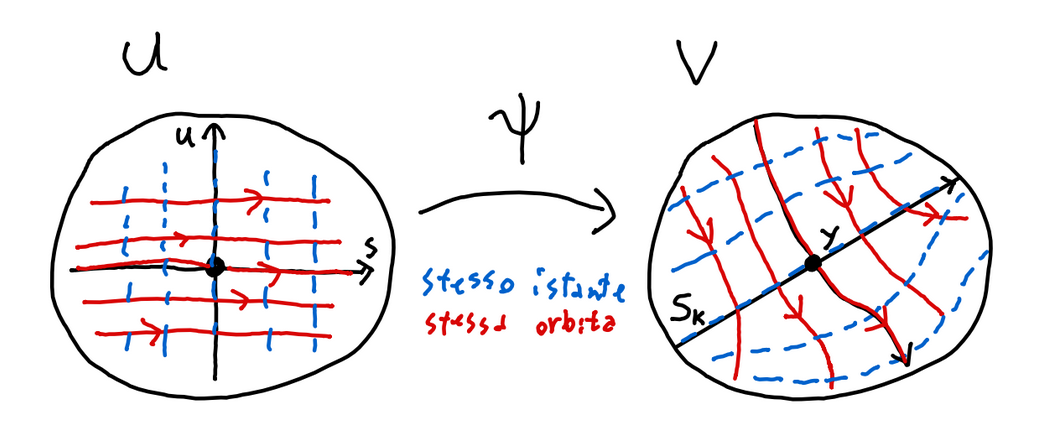
\includegraphics[width=9cm]{Immagini/rettificazione_locale.png}
    \caption{Rappresentazione di come agisce una $\psi$ rettificazione locale come sopra.}
\end{figure}


\begin{theorem}[Poincar\'e-Bendixon]\label{TeoremaPoincareBendixon}
Sia $\dot x=F(x)$ con $F\in C^1(\R^2)$. Supponiamo che esista $D\subseteq \R^2$ compatto non vuoto che non contiene punti fissi e per il quale esiste $x_0\in D$ tale che per qualche $t_0>0$ abbiamo $\phi_t(x_0)\in D$ per ogni $t\geq t_0$.\\
Allora $\Gamma=\omega(x_0)\subseteq D$ \`e un'orbita periodica.
\end{theorem}
\begin{proof}
Sia $x_0\in \R^2$ per cui esiste $t_0>0$ tale che $\phi_t(x_0)\in D$ per ogni $t\geq t_0$. Allora $\omega(x_0)$ \`e non vuoto, invariante e $\omega(x_0)\subseteq D$ per (\ref{OrbitaPositivaLimitataImplicaCompattezzaEInvarianzaOmegaLimite}). Scelto $x\in \omega(x_0)\subseteq D$ allora $\Oc^+(x)\subseteq \omega(x_0)$ e quindi $\omega(x)\subseteq \omega(x_0)$. Sia $y\in \omega(x)$
\vspace{0.25cm}

\noindent
\ul{Claim:} $\#(S_k(y)\cap \Oc^+(x))=1$.
\begin{proof}[Dimostrazione del claim]
Mostriamo prima che l'intersezione \`e non vuota e poi mostriamo che contiene un'unico punto.
\setlength{\leftmargini}{0cm}
\begin{itemize}
\item[$\boxed{\exists}$] Per definizione di $\omega(x)$ esiste una successione monotona $t_k\nearrow +\infty$ tale che $\phi_{t_k}(x)\to y$. Poich\'e $\Nc_{\sigma,\chi}$ \`e un intorno di $y$, per definizione di convergenza esiste $\ol t>\sigma$ tale che $\phi_{\ol t}(x)\in \Nc_{\sigma,\chi}$. Per il lemma sui rettangoli di flusso (\ref{LemmaRettangoliFlusso}) esiste $\wh t\in (-\sigma,\sigma)$ tale che $\phi_{\wh t}(\phi_{\ol t}(x))\in S_k(y)$. Ponendo $\wh t+\ol t=\wt t$ esiste $\wt t>0$ tale che $\phi_{\wt t}(x)\in S_k(y)$.
\item[$\boxed{!}$] Supponiamo per assurdo che esistano $x_1,x_2\in S_k(y)\cap \Oc^+(x)\subseteq \omega(x_0)$ distinti. Per definizione di $\omega$-limite esistono $\tau_{j}^1\nearrow+\infty$ e $\tau_{j}^2\nearrow+\infty$ tali che 
\[\lim_{j\to+\infty}\phi_{\tau^1_j}(x_0)=x_1,\quad \lim_{j\to+\infty}\phi_{\tau^2_j}(x_0)=x_2.\]
Esistono dunque definitivamenteper il lemma sui rettangoli di flusso (\ref{LemmaRettangoliFlusso}) $\wt \tau^1_j$ e $\wt \tau^2_j$ tali che $\phi_{\wt \tau^i_j}(x_0)\in S_k(y)$\footnote{$\wt \tau^i_j\in (\tau^i_j-\sigma,\tau^i_j+\sigma)$}. Siano $U_1$ e $U_2$ intorni di $x_1$ e $x_2$ disgiunti. Per $j$ abbastanza grande abbiamo che $\phi_{\wt \tau^i_j}(x_0)\in U_i$.\\
Poich\'e sia $\wt \tau_j^1$ che $\wt \tau_j^2$ vanno a $+\infty$, esistono $\xi_1<\xi_2<\xi_3$ tali che
\[\phi_{\xi_1}(x_0)\in U_1,\ \phi_{\xi_2}(x_0)\in U_2,\ \phi_{\xi_3}(x_0)\in U_1.\]
Sia $\wt \Gamma$ la curva chiusa data da
\[\wt \Gamma=\cpa{\al\phi_{\xi_1}(x_0)+(1-\al)\phi_{\xi_2}(x_0)\mid \al\in [0,1]}\cup \bigcup_{s\in (\xi_1,\xi_2)}\phi_s(x_0).\]
Per definizione di $S_k(y)$ e per unicit\`a locale si ha che $\Oc^+(\phi_{\xi_2}(x_0))$ \`e contenuto nella componente connessa limitata definita da $\wt \Gamma$, ma questo \`e assurdo perch\'e esiste $\Delta t=\xi_3-\xi_2$ tale che $\phi_{\Delta t}(\phi_{\xi_2}(x_0))=\phi_{\xi_3}(x_0)$ ma per definizione di $S_k(y)$ un'orbita che parte da $S_k(y)$ torna a $S_k(y)$ dal lato opposto rispetto a quello di partenza.
\begin{figure}[!htb]
    \centering
    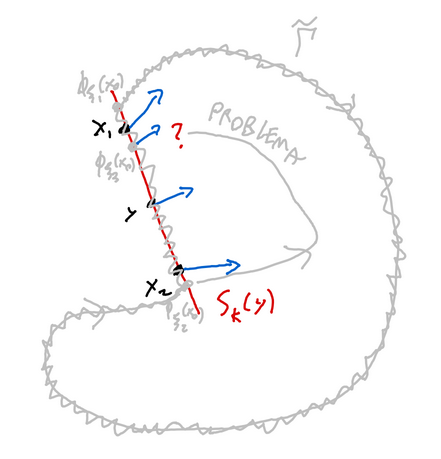
\includegraphics[width=4cm]{Immagini/poincare_bendixon.png}
    \caption{Rappresentazione grafica dell'assurdo trovato.}
\end{figure}

\end{itemize}
\setlength{\leftmargini}{0.5cm}
\end{proof}
\noindent
Sia $y\in \omega(x)$ e sia $\wt t>0$ tale che $\phi_{\wt t}(x)\in S_k(y)$ (esiste per il primo punto del claim). Sappiamo che esiste $\tau>\wt t$ tale che $\phi_{\tau}(x)\in \Nc_{\sigma,\chi}$ (convergenza di successioni). Esiste dunque per il lemma (\ref{LemmaRettangoliFlusso}) un $\wt \tau\in (-\sigma,\sigma)$ tale che $\phi_{\tau+\wt \tau}(x)\in S_k(y)$ e per il secondo punto del claim $\phi_{\tau+\wt\tau}(x)=\phi_{\wt t}(x)$, dunque $\Gamma=\Oc(x)$ \`e periodica.
\vspace{0.25cm}

\noindent
Osserviamo che $\Gamma\subseteq \omega(x_0)$ per costruzione. Mostriamo l'altro contenimento:\\
Sia $z\in \omega(x_0)$ e notiamo che 
\[z=\lim_j \phi_{t_j}(x_0),\qquad x=\lim_{h}\phi_{\tau_h}(x_0).\] 
Ponendo $j(0)=0$, sia $j(h+1)$ il pi\`u piccolo intero tale che $t_{j(h+1)}>t_{j(h)}+\tau_{h+1}-\tau_{h}+1$. Con questa scelta $t_{j(h)}-\tau_h\nearrow +\infty$, quindi possiamo scrivere 
\[z\pasgnl={sottosucc.}\lim_h \phi_{t_{j(h)}}(x_0)=\lim_h\phi_{t_{j(h)}-\tau_h}(x).\]
Poich\'e $\Oc(x)$ \`e un'orbita periodica, $\Oc(x)=\omega(x)$ e questo conclude.
\end{proof}

\begin{remark}
Osserviamo che $D$ come nel teorema di Poicar\'e-Bendixon non pu\`o essere semplicemente connesso per la teoria dell'indice.
\end{remark}

\begin{remark}[Tipico uso di Poincar\'e-Bendixon]
Nel contensto di esercizi, spesso il teorema di Poincar\'e-Bendixon come segue:
\begin{itemize}
\item Ci mettiamo in coordinate polari centrate in un punto fisso instabile isolato.
\item Verifichiamo che esistono $0<\rho_0<\rho_1$ tali che $\cpa{\rho_0\leq\rho\leq \rho_1}$ non contiene punti fissi e (generalmente) 
\[\dot\rho\res{\rho=\rho_0}>0,\qquad\dot \rho\res{\rho=\rho_1}<0.\]
\end{itemize}
\end{remark}

\begin{fact}[Poincar\'e-Bendixon generale]
Se per $x_0$ esiste $t_0>0$ tale che $\phi_t(x_0)\in D$ per ogni $t\geq t_0$ con $D$ non vuoto e compatto allora $\omega(x_0)$ pu\`o essere
\begin{itemize}
\item punto fisso
\item orbita periodica
\item unione di punti fissi e orbite eterocline
\item punto fisso e orbita omoclina
\end{itemize}
\end{fact}

\begin{example}
Consideriamo il sistema
\[\begin{cases}
\dot \rho=\rho(1-\rho^2) + \e f(x,y)\\
\dot \theta=1+\e g(x,y)
\end{cases}\]
Se $f,g\in C^1$ allora esiste $\e_0>0$ tale che per ogni $\e<\e_0$ esiste un orbita periodica.\\
Proviamo a definire
\[D=\cpa{\rho_1\leq\rho\leq\rho_2}\]
Osserviamo che nel caso non perturbato, per $\rho<1$ allora $\dot \rho>0$ mentre per $\rho>1$ allora $\dot \rho<0$.\\
Sia $M=\max\cpa{\norm {f\res{\cpa{\rho\leq 5}}}_\infty, \norm {g\res{\cpa{\rho\leq 5}}}_\infty}$ (dove $5$ \`e un qualche valore ``grosso"). Proviamo a definire $D=\cpa{\frac12\leq \rho\leq 2}$.\\
$\rbar{\dot \rho}_{\rho=\frac12}=\frac38+\e f(\frac12,\theta)\geq \frac38-\e M$ e questo \`e maggiore di $0$ per $\e<\frac3{8M}$.
Similmente per $\rbar{\dot \rho}_{\rho=2}$ chiediamo $\e<\frac6M$. Cerchiamo allora stime tali che
$\rbar{\dot \theta}_{\cpa{\frac12\leq \rho\leq 2}}\neq 0$ e dopo conti simili troviamo che $\e_0=\frac3{8M}$ rispetta tutte le condizioni volute.
\end{example}
\chapter{Esempi di sistemi dinamici continui}

\section{Alcuni sistemi meccanici}
\subsection{L'oscillatore armonico}
Consideriamo l'equazione
\[\ddot x=-kx\]
con $k>0$ e $x\in \R$.\\
Studiamo il sistema equivalente
\[\begin{cases}
\dot x=y\\
\dot y=-kx
\end{cases}\]
con $(x,y)\in\R^2$ e $F(x,y)=(y,-kx)$.

\begin{itemize}
\item \textbf{Punti fissi}: $(y,-kx)=(0,0)\implies (x,y)=(0,0)$, quindi abbiamo un solo punto fisso.
\item Questo \`e evidentemente un sistema meccanico con $V(x)=\frac k2 x^2$, da cui $E(x,y)=\frac12 y^2+\frac k2 x^2$ \`e l'Hamiltoniana.
\item Sia $E_c=\cpa{\frac12y^2+\frac k2x^2=c}$. Questi insiemi sono evidentemente ellissi. Descrivono veramente orbite periodiche? S\`i, infatti se per assurdo non fossero orbite periodiche, poich\'e le orbite che cominciano in uno di questi insiemi sono costrette a rimanervi, per compattezza di $E_c$ dovremmo avere 
\[\ell=\lim_{t\to+\infty}\phi_t(x_0)\in E_c\] 
per $x_0\in E_c$, ma questo significa che $\ell$ sarebbe un punto fisso, che \`e assurdo perch\'e l'unico punto fisso \`e $(0,0)$.
\end{itemize}

\subsection{Pendolo semplice}
L'equazione in esame \`e
\[\ddot \theta=-\frac g\ell\sin\theta.\]
Riformuliamo in
\[\begin{cases}
\dot\theta=\psi\\
\dot\psi=-\frac g\ell\sin\theta
\end{cases}\]

\noindent
\textbf{Punti fissi}:\\
$\psi=0$ e $\sin\theta=0$, dunque
\[pt.fix=\cpa{(k\pi,0)\mid k\in\Z}.\]
\textbf{Integrale primo}:\\
Anche questo \`e un sistema meccanico, che quindi ammette Hamiltoniana
\[E(\theta,\dot\theta)=\frac12\dot\theta^2-\frac g\ell\cos\theta,\]
dunque gli insiemi di livello che ci interessano sono
\[E_c=\cpa{\frac12\psi^2-\frac g\ell\cos\theta=c}.\]
Osserviamo che
\[E(k\pi,0)=-\frac g\ell\cos(k\pi)=(-1)^{k+1}\frac g\ell\implies E(2\pi,0)=E(-2\pi)=E(0,0).\]
\[E_{-\frac{g}{\ell}}=\cpa{\frac12\psi^2-\frac g\ell\cos\theta=-\frac{g}{\ell}}\implies \psi^2=-2\frac g\ell(1-\cos\theta)\]
\[E_{\frac{g}{\ell}}=\cpa{\frac12\psi^2-\frac g\ell\cos\theta=\frac{g}{\ell}}\implies \psi^2=2\frac g\ell(1+\cos\theta)\]
Se $c\in\pa{-\frac g\ell,\frac g\ell}$ troviamo orbite periodiche contenute dentro le ondine dei primi due.\\
Per $c\notin \spa{-\frac g\ell,\frac g\ell}$ abbiamo invece ondine tutte sopra o tutte sotto.
\begin{figure}[!htb]
    \centering
    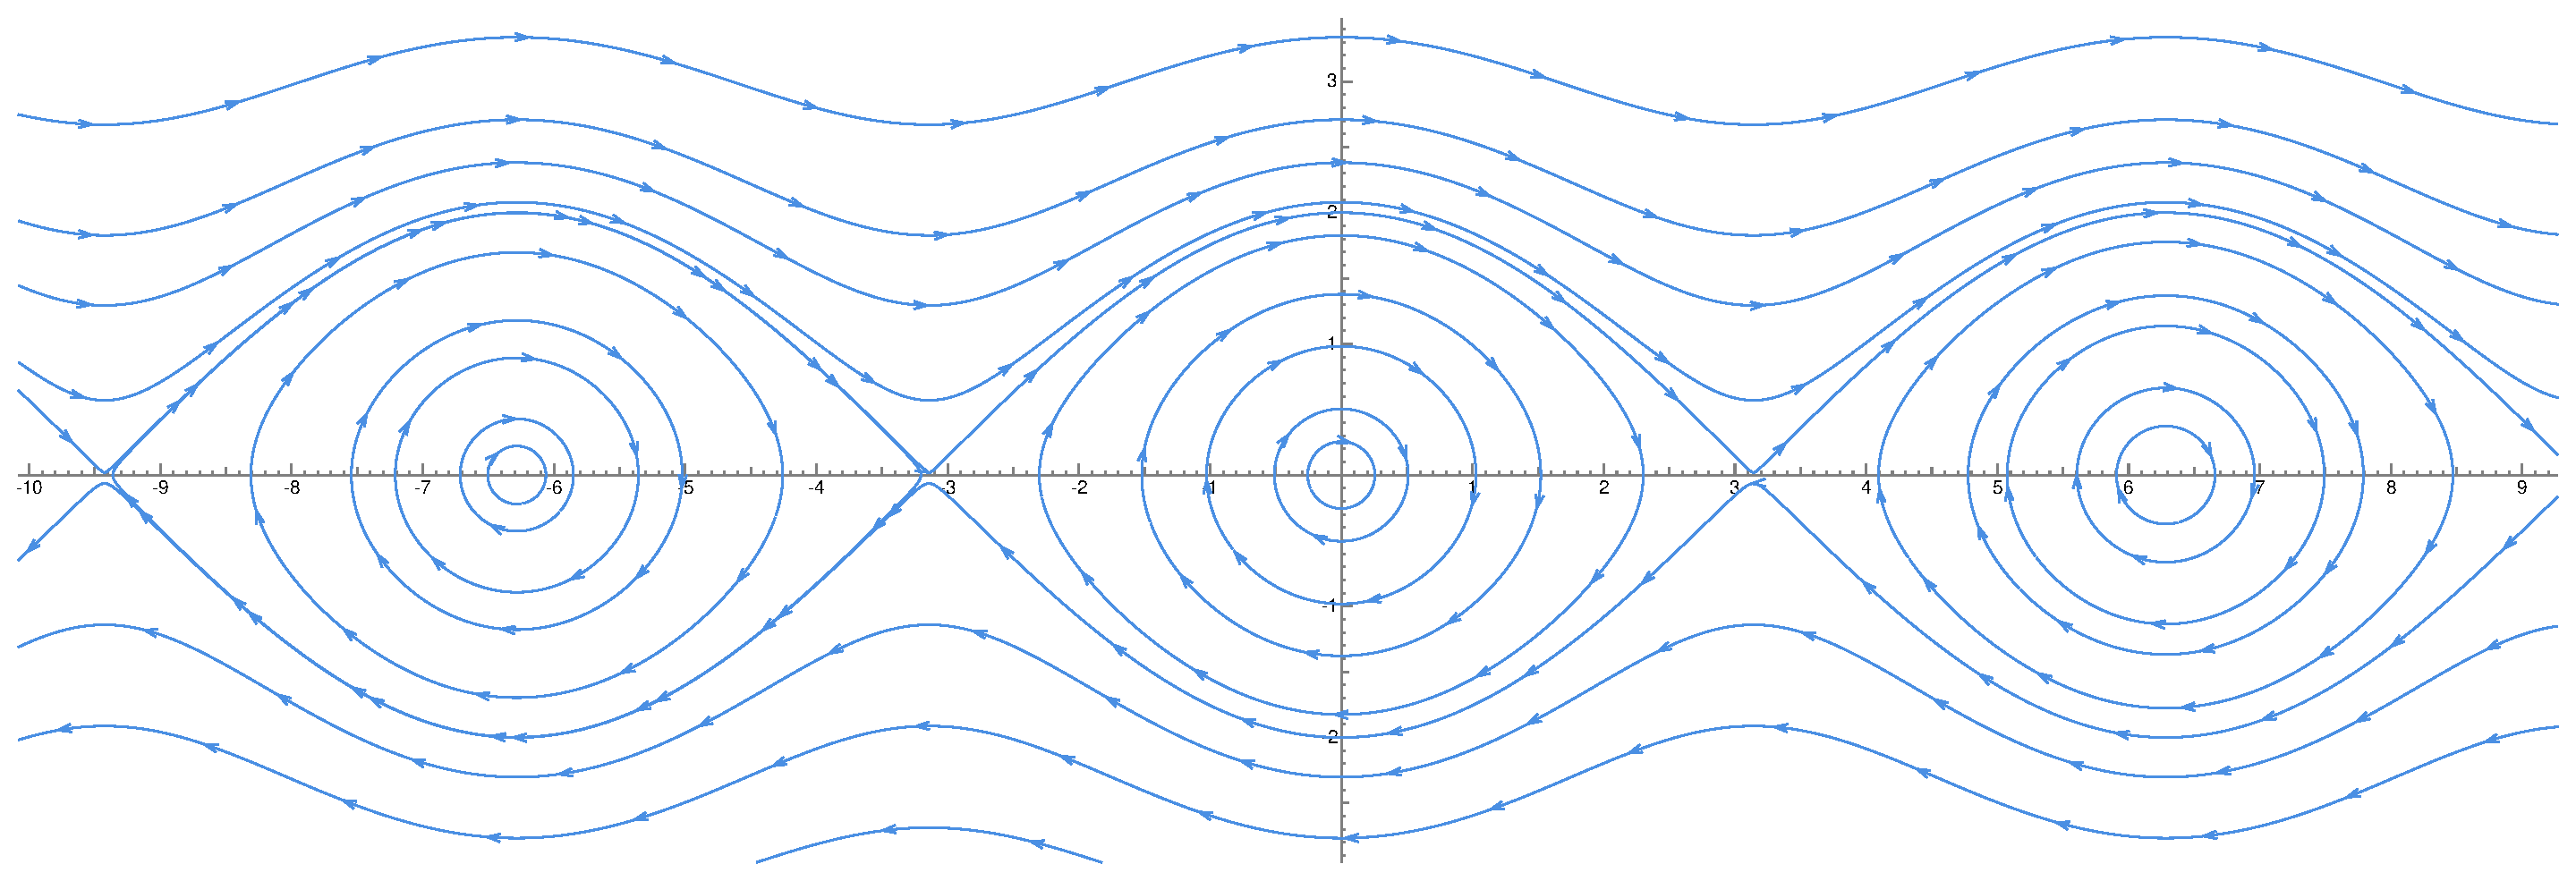
\includegraphics[width=11cm]{Immagini/pendolo.pdf}
    \caption{Diagramma di fase del pendolo per $\frac g\ell=1$}
\end{figure}



\section{Dinamica di Lotka-Volterra}
Possiamo modellare una singola popolazione in modo semplice con l'equazione (detta \textit{equazione logistica})
\[\dot x=x(c-a x),\quad a,c>0.\]
Ponendo $F(x)=xc-ax^2$ si ha che $F(x)=0\implies x=0$ oppure $x=c/a$.\\
Inserendo nel sistema una seconda popolazione che pi\`u interagire con la prima troviamo il sistema
\[\begin{cases}
\dot x=x(c_1-a_1x-b_1y)\\
\dot y=y(c_2-a_2y-b_2x)
\end{cases}.
\]
Osserviamo che gli assi sono invarianti. A meno di riscalamento possiamo considerare il sistema
\[\begin{cases}
\dot x=x(1-x-\al y)\\
\dot y=y(1-\beta x-y)
\end{cases}\]
Troviamo come punti fissi $(0,0)$, $(1,0)$, $(0,1)$ e
\[P=\pa{\frac{\al-1}{\al\beta-1},\frac{\beta-1}{\al\beta-1}}.\]
Osserviamo che $P\in\cpa{x>0,y>0}$ se e solo se $\al>1$ e $\beta>1$ o $0<\al<1$ e $0<\beta<1$.\\
Calcoliamo ora $\Dc F$
\[\Dc F=\mat{1-2x-\al y & -\al x\\ -\beta y & 1-\beta x-2y}.\]
Segue che
\begin{gather*}
\Dc F((0,0))=\mat{1 & 0\\ 0 & 1},\\
\Dc F((1,0))=\mat{-1 & -\al\\ 0 &1-\beta},\quad
\Dc F((0,1))=\mat{1-\al & 0\\ -\beta & -1},\\
\Dc F(P)=\frac 1{\al \beta -1}\mat{
    1-\al &
    \al(1-\al)\\
    \beta(1-\beta) &
    1-\beta
}.
\end{gather*}

\begin{example}
Consideriamo il modello Lotka-Volterra dato da $\al=2$ e $\beta=2$, cio\`e
\[\begin{cases}
\dot x=x(1-x-2y)\\
\dot y=y(1-2x-y)
\end{cases}\]
Per quanto detto sopra i punti fissi sono
\[(0,0),\ (1,0),\ (0,1),\ \pa{\frac13,\frac13},\]
che nominiamo rispettivamente $P_0,\ P_1,\ P_2$ e $P_3$.\\
Segue che $P_0$ \`e una stella instabile, $P_1$ e $P_2$ sono nodi impropri stabili e $P_3$ \`e una sella.
Gli autovettori di $\Dc F(P_3)=-\frac13\pa{\smat{1 &2\\2&1}}$ sono $v_+=(1\ -1)^\top$ e $v_-=(1\ 1)^\top$, corrispondenti agli autovalori $1/3$ e $-1$ rispettivamente. Graficando il sistema possiamo effettivamente notare che le variet\`a instabili e stabili hanno come giacitura della retta tangente in $P_3$ proprio le rette generate da questi vettori.
\begin{figure}[!htb]
    \centering
    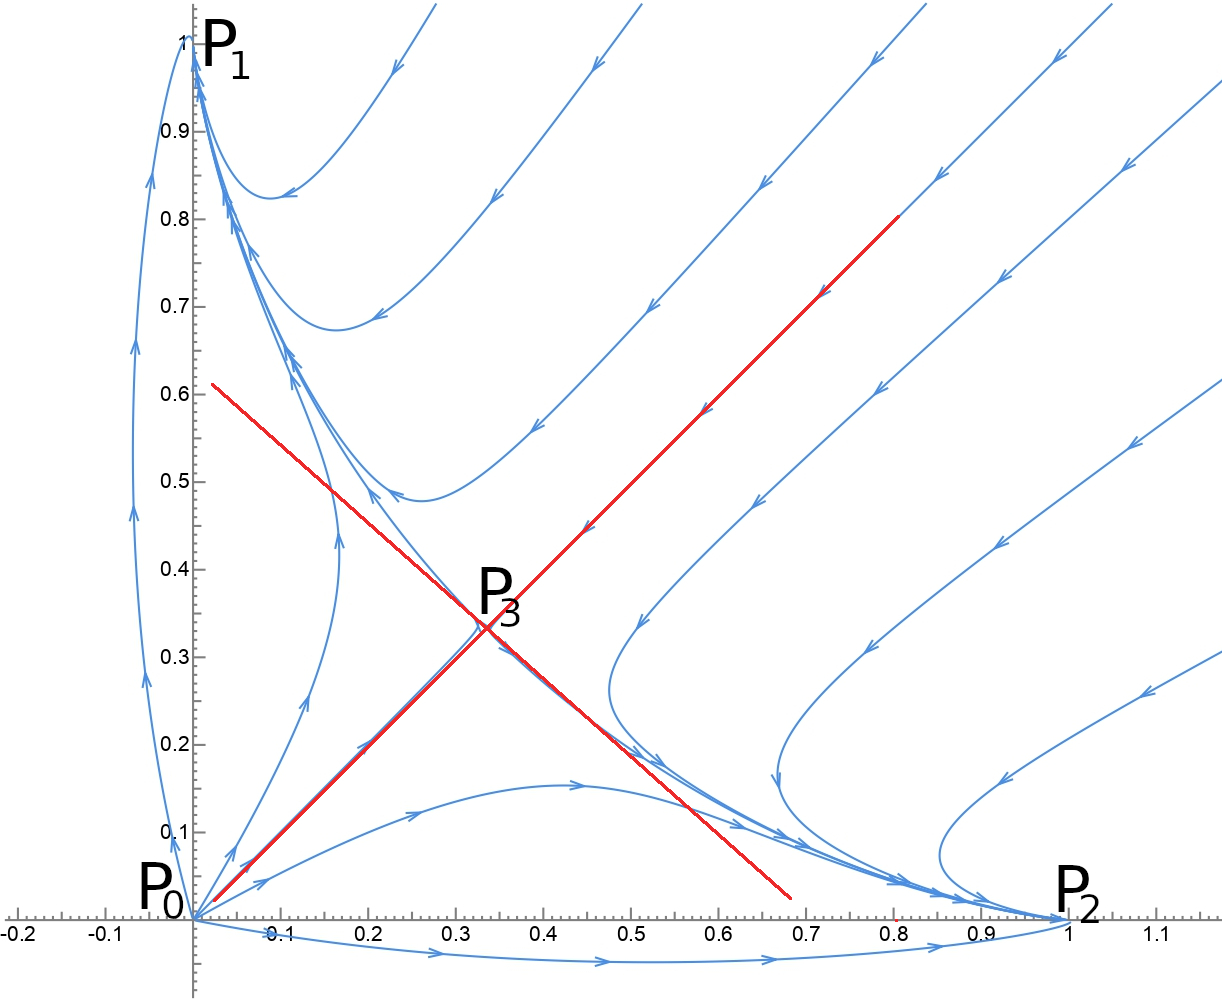
\includegraphics[width=8cm]{Immagini/Lotka-VolterraVarietaStabili.jpg}
    \caption{Diagramma di fase di questo sistema.\\
    In rosso sono indicati $P_3+\Span(v_+)$ e $P_3+\Span(v_-)$.}
\end{figure}

\end{example}

\begin{example}[Lotka-Volterra per preda-predatore]
Consideriamo il sistema
\[\begin{cases}
\dot x= x(-1+y)\\
\dot y=y(1-x)
\end{cases}\]
I punti fissi sono $(0,0)$ e $(1,1)$. Osserviamo anche che gli assi e tutto il primo quadrante sono insiemi invarianti. Consideriamo allora solo il primo quadrante che tanto \`e il caso interessante per questo modello.\\
Studiamo lo Jacobiano
\[\Dc F(x,y)=\mat{-1+y & x\\ -y & 1-x}\implies \Dc F(0,0)=\mat{-1 &0\\0&1},\ \Dc F(1,1)=\mat{0 & 1\\ -1 &0}.\]
\setlength{\leftmargini}{0cm}
\begin{itemize}
\item[$\boxed{(0,0)}$] $(0,0)$ \`e una sella. Si ha che 
\[E^s(0,0)=\Span\mat{1\\0}\quad E^u(0,0)=\Span\mat{0\\ 1}\]
e per il teorema delle variet\`a stabili locali (\ref{TeoremaVarietaStabileInstabile}) sappiamo che $W^s(0,0)$ e $W^u(0,0)$ locali esistono e sono uniche. Per l'invarianza degli assi in realt\`a $W^{u/s}(0,0)=E^{u/s}(0,0)$.
\item[$\boxed{(1,1)}$] $(1,1)$ \`e di tipo centro e quindi non \`e iperbolico. Una possibile funzione di Lyapunov potrebbe avere forma 
\[V(x,y)=a(x-1)^{2n}+b(y-1)^{2m},\quad a,b>0,\ n,m\in \N.\]
Un altro metodo potrebbe essere studiare il punto passando a coordinate polari centrate in $(1,1)$.\\
Un'ulteriore possibilit\`a potrebbe essere studiare il segno del campo di vettori, ma poich\'e $(1,1)$ \`e di tipo centro non \`e molto utile.\\
Trovare insiemi invarianti non \`e molto facile in questo caso.\\
Possiamo provare il metodo delle isocline
\[\begin{cases}
\dd yx=\frac{y(1-x)}{x(-1+y)}\\
y(x_0)=y_0\ t.c. x_0(-1+y_0)
\end{cases}\]
\`E chiaro che possiamo trarre qualche beneficio dal metodo delle isocline perch\'e l'equazione differenziale in questione \`e separabile
\[\frac{-1+y}ydy=\frac{1-x}xdx\implies \int_{y_0}^{y(x)}\frac{-1+y}ydy=\int_{x_0}^{x}\frac{1-x}xdx\]
\[y(x)-\log(y(x))=\log y_0-y_0+\log x-x-\log x_0+x_0.\]
Non posso scrivere esplicitamente $y(x)=$``qualcosa", ma comunque posso studiare l'equazione, infatti, poich\'e $\cpa{y=y(x)}$ \`e invariante (\ref{MetodoIsoclineNelPiano}) sappiamo che c'\`e un insieme invariante. Per identificarlo definiamo
\[I(x,y)=y-\log y+x-\log x.\]
Segue che\footnote{pensando $c=\log y_0-y_0-\log x_0+x_0$}
\[\dot I\res{I=c}=\pa{1-\frac1x}x(-1+y)+\pa{1-\frac1y}y(1-x)=0,\]
cio\`e $I$ \`e un integrale primo.
\[\nabla I(1,1)=\mat{1-\frac1x\\1-\frac1y}\res{(x,y)=(1,1)}=\mat{0\\0}.\]
\[H_I(x,y)=\mat{\frac1{x^2}&0\\ 0&\frac1{y^2}}\res{(x,y)=(1,1)}=\mat{1&0\\0&1}\implies\text{minimo locale}.\]
Troviamo dunque che localmente le traiettorie sono curve semplici chiuse tali che $(1,1)$ si trova nella componente connessa limitata tra le due che hanno come bordo le traiettorie.\\
Per trovare il verso di percorrenza possiamo usare il segno del campo.
\end{itemize}
\setlength{\leftmargini}{0.5cm}
\end{example}


\begin{example}
Un esempio semplice per i parametri del modello sopra \`e
\[\begin{cases}
\dot x=x(3-x-2y)\\
\dot y=y(2-y-x)
\end{cases}\implies F(x,y)=(x(3-x-2y),y(2-x-y)).\]

\begin{figure}[!htb]
    \centering
    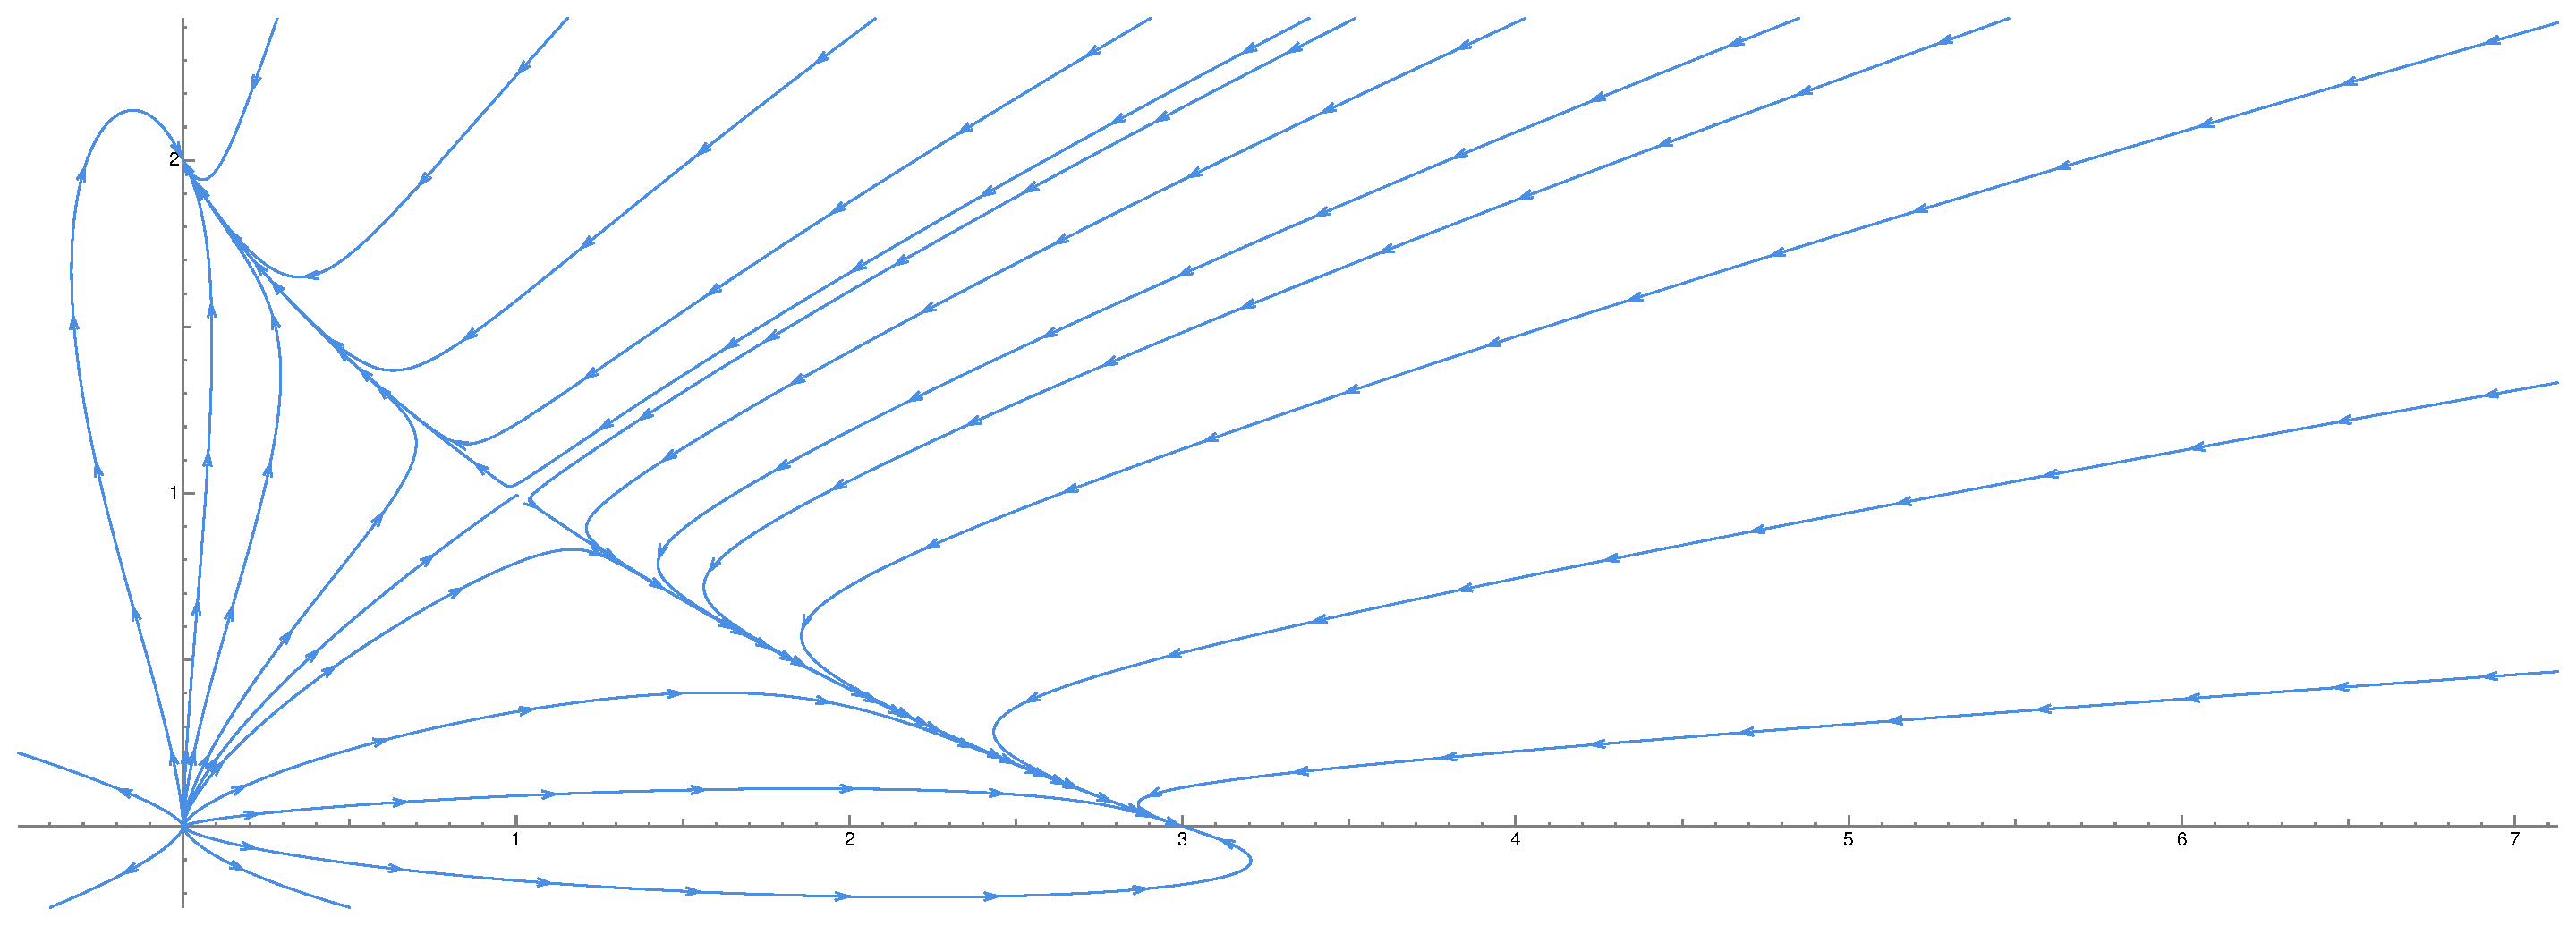
\includegraphics[width=11cm]{Immagini/LotkaVolterra.pdf}
    \caption{Diagramma di fase per questo esempio di Lotka-Volterra.}
\end{figure}

\noindent
I punti fissi sono
\[(0,0),\ (0,2),\ (3,0),\ (1,1)\]
e la matrice Jacobiana di $F$ \`e
\[\Dc F(x,y)=\mat{3-2x-2y & -2x\\
-y & 2-x-2y}.\]
Valutando lo Jacobiano nei punti fissi troviamo
\[\under{\text{nodo instabile}}{\mat{3 & 0\\0&2}},\ \under{\text{nodo stabile}}{\mat{-1 &0\\ -2 &-2}},\ \under{\text{nodo stabile}}{\mat{-3 &-6\\0 &-1}}, \under{\text{sella}}{\mat{-1 & -2\\ -1 & -1}}.\]
\end{example}


\section{Sistema di Lorenz}
Un sistema storicamente importante \`e il seguente:
\[\begin{cases}
\dot x = \sigma(-x+y)\\
\dot y = rx-y-xz\\
\dot z = -bz+xy
\end{cases},\quad r,b,\sigma\in\R^+.\]
Osserviamo che i punti fissi del sistema corrispondono a
\[P_0=\mat{0\\0\\0},\quad P_+=\mat{\sqrt{b(r-1)}\\\sqrt{b(r-1)}\\r-1},\quad P_-=\mat{-\sqrt{b(r-1)}\\-\sqrt{b(r-1)}\\r-1},\]
dove $P_\pm$ \`e definito solo per $r\geq1$. Osserviamo inoltre che
\[\Dc F=\mat{-\sigma&\sigma&0\\r-z&-1&-x\\y&x&-b}.\]
Studiamo la stabilit\`a di $P_0$:\\
Notiamo che
\[\Dc F(P_0)=\mat{-\sigma&\sigma&0\\
r&-1&0\\0&0&-b},\]
dunque $(0,0,1)$ \`e sempre un autovettore relativo all'autovalore $-b$ per il sistema linearizzato vicino a $P_0$. Il segno di $-b$ ci dice che $\dim E^s(P_0)\geq1$. Studiamo la stabilit\`a delle altre direzioni al variare di $r$ 
\setlength{\leftmargini}{0cm}
\begin{itemize}
\item[$\boxed{r\in(0,1)}$] In questo caso gli autovalori sono entrambi con parte reale negativa, quindi per Hartman Grobman (\ref{TeoremaHartmanGrobman}) $P_0$ \`e asintoticamente stabile e $\dim E^s(P_0)=3$.
\item[$\boxed{r>1}$] In questo caso gli autovalori sono reali di segno opposto dunque il punto fisso \`e instabile per Hartman Grobman (\ref{TeoremaHartmanGrobman}) e $\dim E^s(P_0)=2,\ \dim E^u(P_0)=1$.
\item[$\boxed{r=1}$] In questo caso $P_0$ non \`e iperbolico dunque per predicare sulla stabilit\`a proviamo a cercare una funzione di Lyapunov. Tentiamo una di questa forma
\[V(x,y,z)=\frac12(k_1x^2+k_2y^2+k_3z^2).\]
Chiaramente $V$ \`e di classe $C^1$ e $V(P)>V(P_0)=0$ per ogni $P\in\R^3\bs\cpa{P_0}$. Cerchiamo delle condizioni sui $k_i$ in modo tale che $\dot V(P)\leq 0$ per ogni $P\neq P_0$. Dopo qualche conto si pu\`o verificare che
\[V(x,y,z)=\frac12\pa{\frac1\sigma x^2+y^2+z^2}\]
\`e una funzione di Lyapunov (non stretta). Per il primo teorema di Lyapunov (\ref{TeoremaLyapunov1Stabilita}) segue che $P_0$ \`e stabile.\\
Per il criterio di La Salle (\ref{CriterioLaSalle}) sappiamo che $\cpa{\dot V=0}=\cpa{x=y,z=0}$ contiene tutti gli $\omega$-limiti e che questi sono insiemi invarianti. Poich\'e
\[F\res{\cpa{x=y,z=0}}=\mat{0\\0\\x^2}\]
si ha che $\cpa{P_0}$ \`e l'unico insieme invariante contenuto in $\cpa{\dot V=0}$, dunque tutti gli $\omega$-limiti sono $\cpa{P_0}$. Questa condizione insieme alla stabilit\`a di $P_0$ mostra che $P_0$ \`e asintoticamente stabile.
\end{itemize}
\setlength{\leftmargini}{0.5cm}
Attraverso conti non visti a lezione sappiamo che se $\sigma>b+1$ e $r>\ol r$ per un qualche $\ol r>1$ si ha che $\dim E^s(P\pm)=1$ e $\dim E^u(P_\pm)=2$. Le traiettorie dunque approcciano $P_+$ e $P_-$ ``lateralmente" e ``trasversalmente" si allontanano lungo una spirale.

Sempre attraverso conti non visti a lezione individuiamo la funzione
\[W(x,y,z)=\frac12(rx^2+\sigma y^2+\sigma(z-2r)^2),\]
il cui dot \`e dato da
\[\dot W(x,y,z)=-\sigma(rx^2+y^2+b(z-r)^2-br^2).\]
Osserviamo che, fissato $k\in\R^+$ possiamo trovare $c\in\R$ tale che $\dot W\res{W\geq c}\leq -\sigma k<0$: basta prendere $c$ grande abbastanza in modo tale che i punti fuori l'ellissoide $\cpa{W=c}$ abbiano coordinate grandi abbastanza da forzare la disuguaglianza voluta, che possiamo fare per il segno dei termini in $\dot W$.\\
Osserviamo che se $y_0\notin \cpa{W\geq c}$ allora
\[W(\phi_t(y_0))-W(y_0)=\int_0^t\under{=\dot W}{\dd s{}W(\phi_s(y_0))}ds\leq -k\sigma t\]
finch\'e $\phi_t(y_0)$ continua ad essere fuori l'ellissoide. Segue dunque che definitivamente $\phi_t(y_0)$ cade nell'ellissoide.

Questo ragionamento mostra che tutti i punti ammettono $\omega$-limite, ma questo non pu\`o in generale essere un punto fisso (sono instabili) o un'orbita periodica (perch\'e assenti dal sistema\footnote{questa affermazione non \`e stata mostrata}). Si scopre che l'$\omega$-limite generale corrisponde ad un frattale e per questo motivo viene detto \textit{attrattore strano}.

\begin{figure}[!htb]
    \centering
    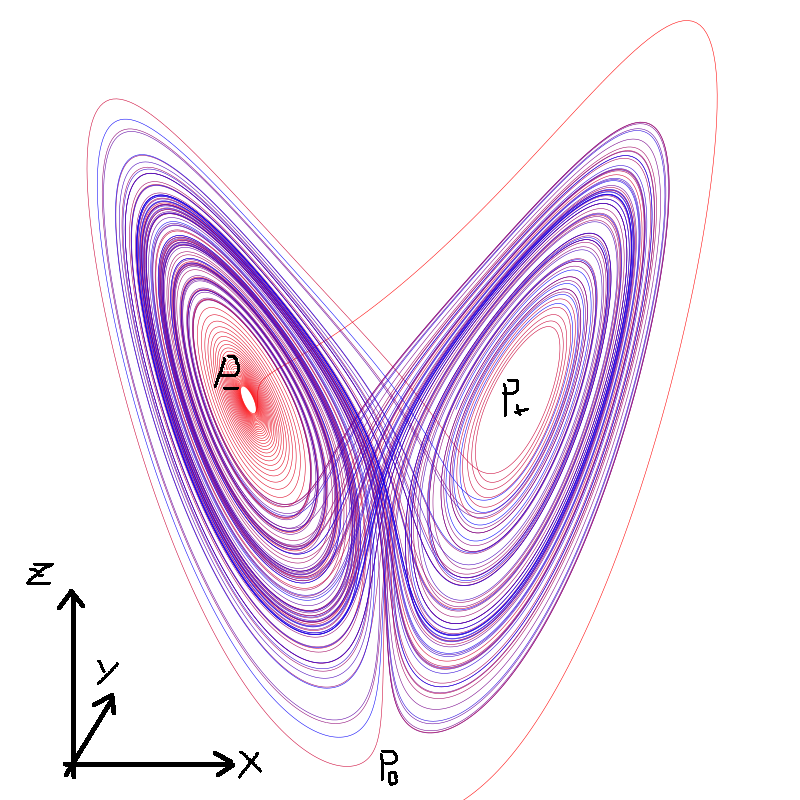
\includegraphics[width=8cm]{Immagini/800px-Lorenz_attractor.png}
    \caption{Qualche orbita del sistema di Lorenz dove sono stati contrassegnati i punti fissi. Immagine originariamente da \url{https://en.wikipedia.org/wiki/Lorenz_system} e modificata da me.}
\end{figure}





\part{Sistemi discreti}

\chapter{Motivazione e basi}


\section{Mappa di Poincar\'e}
Proviamo a capire quando un sistema di equazioni differenziali porta un'orbita a tornare vicino a se stessa.

\begin{definition}[Mappa di Poincar\'e]
Sia $M$ una variet\`a e sia $\Sigma$ una sua sottovariet\`a di codimensione 1 tale che esiste $U\subseteq \Sigma$ con la seguente propriet\`a:\\
se $P\in U$ allora esiste $\ol t>0$ tale che $t\in (0,\ol t)\implies \phi_t(P)\notin U$ e $\phi_{\ol t}(P)\in U$\footnote{$\ol t$ \`e l'istante del ``primo ritorno"}.\\
Definiamo la \textbf{mappa di Poincar\'e} come
\[P_U:\funcDef{U}{U}{(x,y)}{\phi_{\ol t}(x,y)}.\]
\end{definition}
\begin{remark}
Se $P_\Sigma^n=\under{n\text{ volte}}{P_\Sigma\circ\cdots\circ P_\Sigma}$, ponendo $P_\Sigma^0=id$ stiamo definendo un sistema discreto $(\Sigma,P_\Sigma,\Z)$\footnote{$P_\Sigma^{-1}$ \`e definita perch\'e sono partito da un flusso e posso prendere tempi negativi in un flusso}.
\end{remark}

\begin{example}[Moto sul toro piatto]
Sia $T^2=\R^2/\Z^2$. Un moto geodetico sul toro (piatto) si pu\`o pensare come
\[t\mapsto \phi_t(x,y)=(x,y)+t(v_x,v_y)\mod{\Z^2}.\]
Sia $\Sigma=U=S^1=\quot{[0,1]\times\cpa0}{(0,0)\sim(1,0)}$. Per la geometria del toro questa sottovariet\`a di $T^2$ ha le propriet\`a richieste per definire la mappa di Poincar\'e (addirittura sappiamo che $\ol t=1/v_y$).\\
Esplicitamente troviamo che 
\[P_\Sigma:\funcDef{S^1}{S^1}{t}{t+\al \mod 1}\]
dove $\al=v_x/v_y$. Osserviamo che a meno di traslare modulo 1, tutte le orbite sono determinate dall'orbita di $0$.
\setlength{\leftmargini}{0cm}
\begin{itemize}
\item[$\boxed{\al\in\Q}$] Se $\al=\frac pq$ ridotta ai minimi termini allora $P_\Sigma^q(0)=0+p=0 \mod 1$ e le orbite sono periodiche.
\item[$\boxed{\al\in\R\bs\Q}$] Evidentemente non troviamo un'orbita periodica. \`E possibile mostrare che in realt\`a l'orbita \`e densa.
\end{itemize}
\setlength{\leftmargini}{0.5cm}
\end{example}


\begin{definition}[Semipiano di Poincar\'e]
Consideriamo la regione $[-1,1]\times [0,+\infty]\bs D^1$ e identifichiamo i lati come in figura
\begin{figure}[!htb]
    \centering
    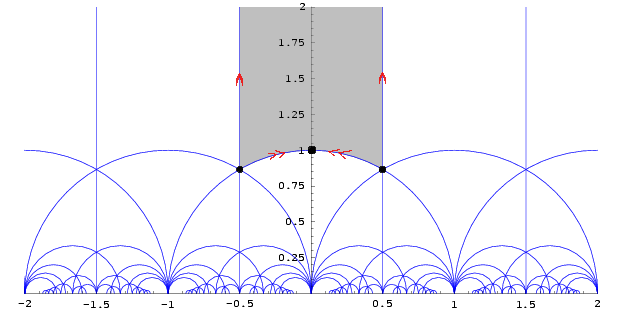
\includegraphics[width=9cm]{Immagini/ModularGroup-FundamentalDomain-01.png}
    \caption{Dominio fondamentale e qualche geodetica.}
    \label{SemipianoPoincare}
\end{figure}

\noindent
Le geodetiche sono le intersezioni dell'oggetto con rette verticali o semicirconferenze perpendicolari all'asse $x$.
Chiamiamo $\Mc$ questo spazio.
\end{definition}
\begin{example}[Geodetiche sul piano di Poincar\'e]
A parte le geodetiche corrispondenti a rette verticali, ogni geodetica che incontra la regione lo fa passando per l'asse $y$ (e quindi lo fa ad un certo angolo). Possiamo associare ad ogni coppia punto di $\Mc$ e angolo una geodetica di $\Mc$ (quella passante per il punto che incontra la verticale a quell'angolo)
\[\Mc\times S^1\ni ((x,y),\theta)\mapsto g_t((x,y),\theta).\]
Sia $\Sigma=\cpa{x=0,y>1}\times S^1$. \`E possibile definire $P_\Sigma$ e si da il caso che questa mappa di Poincar\'e \`e pi\`u facile da studiare rispetto al sistema originale.
\end{example}

\section{Esempi di sistemi discreti caotici}
\begin{example}[Perdo il controllo]
Consideriamo la mappa
\[T:\funcDef{S^1}{S^1}{x}{10x \mod 1}.\]
Poniamo $\Ac=\cpa{0,\cdots,9}$ e $\Ac_n=\pa{\frac n{10},\frac{n+1}{10}}$ per $n\in\Ac$.\\
Sia $x\in \R\bs \Q$ e diamo la seguente mappa
\[\vp:x\mapsto(\omega_0,\omega_1,\cdots)\in \Ac^{\N}\]
dove $\omega_n=k\coimplies T^n(x)\in \Ac_k\coimplies \lfloor10 T^n(x)\rfloor=k$ e per ricorsione vediamo che $\omega_n$ \`e la $n$-esima cifra decimale di $x$, cio\`e
\[x=0.\omega_0\omega_1\omega_2\cdots.\]
Per rispondere ad una domanda del tipo ``$T^{1000}(x)\in \Ac_i?$" devo sapere la 1000-esima cifra di $x$. Se ora considero $x+\e$ al posto di $x$, le informazioni che avevamo su $x$ non dicono pi\`u nulla sul comportamento di $x+\e$ oltre un certo passo\footnote{se $i>-\log_{10} \e$ la risposta a ``$T^{1000}(x)\in \Ac_i?$" e quella a ``$T^{1000}(x+\e)\in \Ac_i?$" sono indipendenti.}.
\end{example}

\begin{remark}[Piccola parentesi statistica]
Sia $x=0.x_1x_2\cdots$ potremmo chiederci, fissata una cifra $k$ se
\[Prob\cpa{\lim_{N\to+\infty}\frac{\#\cpa{i\in \cpa{0,\cdots, N-1}\mid x_i=k}}{N}=\frac1{10}}=1\]
ed effettivamente \`e vero. Segue dunque che
\[Prob\cpa{\lim_{N\to+\infty}\frac{\#\cpa{i\in \cpa{0,\cdots, N-1}\mid x_i=k}}{N}=\frac1{9}}=0\]
anche se non \`e un insieme vuoto\footnote{per esempio posso fissare ogni nona cifra a $k$ e completare le altre con cifre a caso diverse da $k$.}.
\end{remark}

\begin{example}[Oscillatore armonico perturbato]
Sia $f:\R\to \R$ una funzione $1$-periodica. Immaginiamo una palla che rimbalza su un piatto la cui altezza varia come $f$. Per semplificarci la vita possiamo immaginare che l'urto avvenga sempre in $x=0$, tanto l'unica cosa che conta \`e $\dot f$ (l'impulso). Siano $t_0,t_1,\cdots,t_n$ i tempi di urto ($t_0=0$) e siano $v_0,\cdots,v_n$ le velocit\`a dopo l'urto. Conoscendo questi dati possiamo ricostruire tutta la dinamica.
\[T:\funcDef{[0,+\infty)\times (0,+\infty)}{[0,+\infty)\times (0,+\infty)}{(t_{n},v_n)}{(t_{n+1},v_{n+1})}.\]
Calcoliamo
\[\begin{cases}
t_{n+1}=t_n+h(v_n)\\
v_{n+1}=v_n+2\dot f(t_{n+1})
\end{cases},\quad h(v_n)=\frac 2gv_n\]
Osserviamo inoltre che
\[T(t_n+1,v_n)=(t_n+1+h(v_n), v_n+2\dot f(t_n+1 h(v_{n+1})))=T(t_n,v_n)+(1,0),\]
quindi in realt\`a possiamo considerare $S^1$ al posto di $[0,+\infty)$ per i tempi.\\
Questo sistema \`e difficile da trattare e presenta molti problemi aperti.
\end{example}






\appendix
\chapter{Riconoscimenti e risorse}
\section*{Riconoscimenti}
Ringrazio i seguenti colleghi per aver segnalato ambiguit\`a e/o errori:
\begin{center}
Poletti Leonardo.
\end{center}
\section*{Risorse}
Per realizzare le immagini di sistemi bidimensionali ho usato il sito \url{https://paolini.github.io/funplot/}.
\section*{Fonti delle immagini}
Crediti per le immagini non realizzate da me:
\begin{itemize}
\item Figura \ref{SemipianoPoincare}:\\
Fropuff, CC BY-SA 3.0 \url{http://creativecommons.org/licenses/by-sa/3.0/}, via Wikimedia Commons con alcune modifiche del sottoscritto.\\
La pagina di Wikipedia Commons rilevante \`e \url{https://commons.wikimedia.org/wiki/File:ModularGroup-FundamentalDomain-01.png}.
\end{itemize}



\end{document}
